\documentclass[a4,twocolumn,10pt]{article}
\usepackage{usenix2019_v3}
%\documentclass[conference]{IEEEtran}
%\newcommand{\subparagraph}{}
%\usepackage[letterpaper, total={6.5in, 9in}, columnsep=0.25in]{geometry}
%\usepackage[letterpaper, total={7in, 9in}, columnsep=0.33in]{geometry}
%\usepackage[letterpaper, total={7.15in, 9.5in}, columnsep=0.15in]{geometry}
\newcommand{\tronly}[2]{#1}
\usepackage{newtxtext}
\usepackage{appendix}
\tronly{}{%
%\usepackage{microtype}
\usepackage[subtle]{savetrees}
}
\usepackage{comment}
\usepackage{mathtools}
\usepackage{fancyvrb}
\DeclarePairedDelimiter{\ceil}{\lceil}{\rceil}
\DeclarePairedDelimiter{\floor}{\lfloor}{\rfloor}

\setlength{\parskip}{0pt}
\setlength{\abovedisplayskip}{3pt}
\setlength{\belowdisplayskip}{3pt}
\setlength{\textfloatsep}{2pt plus 1.0pt minus 1.0pt}
\setlength{\floatsep}{2pt plus 1.0pt minus 1.0pt}
%\setlength{\textfloatsep}{1pt plus 0.0pt minus 1.0pt}
%\setlength{\floatsep}{1pt plus 0.0pt minus 1.0pt}

\usepackage{cite}
\usepackage{paralist}
%\usepackage[hyphens]{url}
\usepackage[compact]{titlesec}
\usepackage{enumitem}
\setdefaultleftmargin{0em}{}{}{}{}{}
\setdefaultitem{{}}{}{}{}
\setlist[itemize]{leftmargin=*}
\setlist[enumerate]{leftmargin=*}
%\expandafter\def\expandafter\UrlBreaks\expandafter{\UrlBreaks%  save the current one
%\do\a\do\b\do\c\do\d\do\e\do\f\do\g\do\h\do\i\do\j%
%\do\k\do\l\do\m\do\n\do\o\do\p\do\q\do\r\do\s\do\t%
%\do\u\do\v\do\w\do\x\do\y\do\z\do\A\do\B\do\C\do\D%
%\do\E\do\F\do\G\do\H\do\I\do\J\do\K\do\L\do\M\do\N%
%\do\Oh\do\P\do\Q\do\R\do\S\do\T\do\U\do\V\do\W\do\X%
%\do\Y\do\Z}
\usepackage{caption}
% \captionsetup[figure]{font=small,labelfont=small,skip=3pt}
\usepackage[normalem]{ulem}
\usepackage{amsmath}
\usepackage{bbm}
\usepackage{thmtools, thm-restate}
\usepackage{mathrsfs}
\usepackage{amssymb}
\usepackage{tikz}
\usepackage{dsfont}
\usepackage{capt-of}
\usepackage{algorithmicx}
\usepackage{algorithm}
\usepackage[noend]{algpseudocode}
\usepackage{amsthm}
\usepackage[makeroom]{cancel}
\usepackage{datetime}
\renewcommand\ttdefault{cmtt}
\graphicspath{{./figures}}
\DeclareMathOperator*{\argmin}{arg\,min}
\DeclareMathOperator*{\argmax}{arg\,max}
\newcommand{\Oh}[1]{O(#1)}
\let\oldemptyset\emptyset
\let\emptyset\varnothing
% New definitions
\algnewcommand\algorithmicswitch{\textbf{switch}}
\algnewcommand\algorithmiccase{\textbf{case}}
\algnewcommand\algorithmicassert{\texttt{assert}}
\algnewcommand\Assert[1]{\State \algorithmicassert(#1)}%
% New "environments"
\algdef{SE}[SWITCH]{Switch}{EndSwitch}[1]{\algorithmicswitch\ #1\ \algorithmicdo}{\algorithmicend\ \algorithmicswitch}%
\algdef{SE}[CASE]{Case}{EndCase}[1]{\algorithmiccase\ #1}{\algorithmicend\ \algorithmiccase}%
\algtext*{EndSwitch}%
\algtext*{EndCase}%⇧
\algnewcommand\algorithmiccontinue{\textbf{continue}}
\algnewcommand\algorithmicbreak{\textbf{break}}
\algnewcommand\Continue{\algorithmiccontinue}
\algnewcommand\Break{\algorithmicbreak}
\newcommand{\editremove}[1]{{\color{red}\sout{#1}}}
\newcommand{\editinsert}[1]{{\color{blue}#1}}
\newcommand{\editchange}[1]{{\color{orange}#1}}
\newcommand\ddfrac[2]{\frac{\displaystyle #1}{\displaystyle #2}}

%O \newtheorem{theorem}{Theorem}
\newtheorem{theorem}{Théorème}
%O \newtheorem{lemma}[theorem]{Lemma}
\newtheorem{lemma}[theorem]{Lemme}
\newtheorem{conjecture}[theorem]{Conjecture}
%O \theoremstyle{definition}
\theoremstyle{definition}
%O \newtheorem{definition}{Definition}[section]
\newtheorem{definition}{Définition}[section]

\newcommand\blfootnote[1]{%
  \begingroup
  \renewcommand\thefootnote{}\footnote{#1}%
  \addtocounter{footnote}{-1}%
  \endgroup
}

% Default section titles for French version
\renewcommand{\abstractname}{Résumé}
\renewcommand{\refname}{Références}
\renewcommand{\proofname}{Preuve}

\settimeformat{hhmmsstime}
\mmddyyyydate
\title{
%O \Large\bf Scalable and Probabilistic Leaderless BFT Consensus through Metastability}
\Large\bf Consensus BFT sans dirigeant extensible et probabiliste par métastabilité}
\author{%
\tronly{%
Team~Rocket,
Maofan~Yin,
Kevin~Sekniqi,
Robbert~van~Renesse,
Emin~G\"un~Sirer\\
Cornell University\textsuperscript{*}\\
\small{Traduit par Grégory Lemercier et Jean Zundel}
}{%
Anonymous Submission 134
}
}
\date{}

\tronly{%
\usepackage[hang]{footmisc}
\setlength\footnotemargin{0em}
}

\begin{document}
\maketitle
\tronly{%
\blfootnote{%
%O \textsuperscript{*}\emph{Blasts off at the speed of light!} --- Team Rocket\\
\textsuperscript{*}\emph{À la vitesse de la lumière !} --- Team Rocket\\
%O An earlier version of this paper published on May 16th 2018, IPFS, was titled \emph{Snowflake to Avalanche: A Novel Metastable Consensus Protocol Family for Cryptocurrencies}.
Une version antérieure de cet article, publié le 16 mai 2018, IPFS, était intitulée \emph{Snowflake to Avalanche: A Novel Metastable Consensus Protocol Family for Cryptocurrencies}.

%Proof of Team Rocket: \verb|SHA256("avalanche ted yin kevin sekniqi robbert van |\\
%\verb|renesse emin gun sirer\n") = 0x 8a5d 2d32 e68b c500 36e4 |\\
%\verb|d086 0446 17fe 4a0a 0296 b274 999b a568 ea92 da46 d533|
}
}{}

\begin{abstract}
%O This paper introduces a family of leaderless Byzantine fault tolerance protocols, built around a metastable mechanism via network subsampling.
Cet article présente une famille de protocoles à tolérance de faute byzantine sans dirigeant, bâtis autour d'un mécanisme métastable \emph{via} sous-échantillonnage réseau.
%O These protocols provide a strong probabilistic safety guarantee in the presence of Byzantine adversaries while their concurrent and leaderless nature enables them to achieve high throughput and scalability.
Ces protocoles fournissent une forte garantie de sûreté probabiliste en présence d'adversaires byzantins, tandis que leur nature simultanée et sans dirigeant leur permet d'être performants et extensibles.
%O Unlike blockchains that rely on proof-of-work, they are quiescent and green.
Contrairement aux blockchains fondées sur la preuve de travail (\emph{proof-of-work}), ils sont économes et écologiques.
%O Unlike traditional consensus protocols where one or more nodes typically process linear bits in the number of total nodes per decision, no node processes more than logarithmic bits. It does not require accurate knowledge of all participants and exposes new possible tradeoffs and improvements in safety and liveness for building consensus protocols.
Contrairement aux protocoles de consensus traditionnels où, typiquement, un ou plusieurs nœuds traitent linéairement l'information pour chaque décision, aucun nœud ne traite l'information d'une manière plus complexe que logarithmique. Il ne requiert pas de connaissance précise de tous les participants et propose de nouveaux compromis et améliorations en termes de sûreté de fonctionnement et de vitalité pour la construction de nouveaux protocoles de consensus.
%Finally, unlike traditional consensus protocols and similar to longest-chain protocols, our protocols provide increase in both liveness and safety guarantees when the observed adversarial presence decreases below the maximal expected bound. 

%where $k$ is dependent on the security requirements of the system.
% require $O(n^{2})$
% communication, their communication complexity ranges from
% $O(kn\log n)$
% to
% $O(kn)$
% for some security parameter $k \ll n$. \Jon{This sentence led me to assuem that the two ``best'' protocols were both going to be important; that there would be a reason to use the $O(kn\log n)$ version despite its poorer aymptotics. But when I got to later pages, I see you're only discussing Avalanche after all; the other algorithms are purely steps on the pedagogical garden path, right? Maybe remove the reference to the intermediate steps from the abstract?} 

%O The paper describes the Snow protocol family, analyzes its guarantees, and describes how it can be used to construct the core of an internet-scale electronic payment system called Avalanche, which is evaluated in a large scale deployment.
Cet article décrit la famille de protocoles Snow, analyse ses garanties et décrit la manière dont il peut être employé pour bâtir le cœur d'un système de paiement électronique à l'échelle de l'internet appelé Avalanche, lequel est évalué lors d'un déploiement à grande échelle.
%O Experiments demonstrate that the system can achieve high throughput (3400 tps), provide low confirmation latency (1.35 sec), and scale well compared to existing systems that deliver similar functionality. For our implementation and setup, the bottleneck of the system is in transaction verification.
Les expériences montrent que le système peut atteindre un haut débit (3400~tps), fournir une faible latence de confirmation (1,35~s) et correctement passer à l'échelle par rapport à d'autres systèmes offrant des fonctionnalités similaires. Le goulet d'étranglement du système dans l'implémentation et la configuration retenues est la vérification des transactions.
\end{abstract}

\section{Introduction}

%O Achieving agreement among a set of distributed hosts lies at the core of countless applications, ranging from Internet-scale services that serve billions of people~\cite{Burrows06,HuntKJR10} to cryptocurrencies worth billions of dollars~\cite{marketcapcryptocurrency}.
L'obtention d'un accord au sein d'un ensemble d'hôtes distribués se retrouve au cœur d'innombrables applications allant de services à l'échelle de l'Internet servant des milliards de gens~\cite{Burrows06,HuntKJR10} à des cryptomonnaies valant des milliards de dollars~\cite{marketcapcryptocurrency}.
%O To date, there have been two main families of solutions to this problem.
À ce jour, il existe deux familles principales de solutions à ce problème.
%O Traditional consensus protocols %, exemplified by PBFT~\cite{castro1999practical},
%O rely on all-to-all communication to ensure that all correct nodes reach the same decisions with absolute certainty.
Les protocoles de consensus traditionnels
sont fondés sur une communication entre chaque pair pour s'assurer que tous les nœuds correct arrivent aux mêmes décisions avec une certitude absolue.
%Because they usually require quadratic communication overhead and accurate knowledge of membership, they have been difficult to scale
%O to large numbers of participants.
Comme ils impliquent en général un nombre de communications croissant de façon quadratique et une connaissance exacte des membres du réseau, il s'est avéré difficile de l'étendre
à de nombreux participants.
%O On the other hand, Nakamoto consensus protocols~\cite{nakamoto2008bitcoin,GarayKL15, PassSS17, SompolinskyZ15, SompolinskyLZ16, SompolinskyZ18, BentovHMN17, EyalGSR16,Kokoris-KogiasJ16,PassS16a, PassS18} have become popular with the rise of Bitcoin.
D'un autre côté, les protocoles de consensus Nakamoto~\cite{nakamoto2008bitcoin,GarayKL15, PassSS17, SompolinskyZ15, SompolinskyLZ16, SompolinskyZ18, BentovHMN17, EyalGSR16,Kokoris-KogiasJ16,PassS16a, PassS18} ont été popularisés par Bitcoin.
%O These protocols provide a probabilistic safety guarantee: Nakamoto consensus decisions may revert with some probability $\varepsilon$.
Ces protocoles fournissent une garantie de sûreté probabiliste\,: les décisions par consensus Nakamoto peuvent s'inverser avec une certaine probabilité $\varepsilon$.
%O A protocol parameter allows this probability to be rendered arbitrarily small, enabling high-value financial systems to be constructed on this foundation.
Un paramètre du protocole permet d'abaisser à volonté cette probabilité, ce qui permet de bâtir des systèmes financiers de grande valeur sur ces fondations.
%O This family is a natural fit for open, permissionless settings where any node can join the system at any time.
Cette famille est conçue pour des configurations ouvertes et en libre accès où tout nœud peut rejoindre le système à tout moment.
%O Yet, these protocols are costly, wasteful, and limited in performance.
Cependant ces protocoles sont coûteux, gaspilleurs et limités en performance.
%O By construction, they cannot quiesce: their security relies on constant participation by miners, even when there are no decisions to be made.
Par construction, ils sont tenus de fonctionner même à vide\,: leur sécurité se base sur une participation constante des mineurs, même quand aucune décision ne doit être prise.
%O Bitcoin currently consumes around 63.49 TWh/year~\cite{bitcoinpower}, about twice as all of Denmark~\cite{denmarkpower}.
Bitcoin consomme actuellement autour de 63.49 TWh/an~\cite{bitcoinpower}, environ deux fois l'énergie consommée par le Danemark~\cite{denmarkpower}.
%O Moreover, these protocols suffer from an inherent scalability bottleneck that is difficult to overcome through simple reparameterization~\cite{CromanDEGJKMSSS16}. % \Jon{I wanted the paper to expand on this point, but I missed it.}
De plus, ces protocoles souffrent d'un goulet d'étranglement intrinsèque pour le passage à l'échelle qui s'avère difficile à dépasser par la simple reparamétrisation~\cite{CromanDEGJKMSSS16}.
%O This paper introduces a new family of consensus protocols called Snow.
Cet article présente une nouvelle famille de protocoles de consensus appelés Snow.
%O Inspired by gossip algorithms, this family gains its properties through a deliberately metastable mechanism.
Inspirée par les algorithmes de \emph{gossip} ou bavardage, cette famille possède des propriétés grâce à un mécanisme délibérément métastable.
%O Specifically, the system operates by repeatedly sampling the network at random, and steering correct nodes towards a common outcome.
En particulier, le système opère en échantillonnant répétitivement le réseau au hasard, et en dirigeant les nœuds corrects vers un résultat commun.
%O Analysis shows that this metastable mechanism is powerful: it can move a large network to an irreversible state quickly, where the irreversibility implies that a sufficiently large portion of the network has accepted a proposal and a conflicting proposal will not be accepted with any higher than negligible ($\varepsilon$) probability. 
L'analyse montre que ce mécanisme métastable est puissant\,: il peut rapidement changer l'état d'un vaste réseau de manière irréversible, où l'irréversibilité implique qu'une part suffisamment importante du réseau a accepté une proposition et qu'une proposition différente ne sera acceptée qu'avec une probabilité au maximum négligeable.
%{\color{red} We should clarify this.  The current statement is too strong.}
% though it is not always guaranteed to do so.
% \Jon{Not universal in that some applications require a hard guarantee?}

%O Similar to Nakamoto consensus, the Snow protocol family provides a probabilistic safety guarantee, using a tunable security parameter that can render the possibility of a consensus failure arbitrarily small.
De même que le consensus Nakamoto, la famille des protocoles Snow fournissent une garantie de sûreté probabiliste, grâce à un paramètre de sécurité configurable qui peut amenuiser à volonté la possibilité d'un échec du consensus.
%O Unlike Nakamoto consensus, the protocols are green, quiescent and efficient; they do not rely on proof-of-work~\cite{DworkN92} and do not consume energy when there are no decisions to be made.
Contrairement au consensus Nakamoto, ces protocoles sont écologiques, économes et efficients\,; ils ne dépendent pas d'une preuve de travail\cite{DworkN92} et ne consomment pas d'énergie quand il n'y a pas de décision à prendre.
%0 The efficiency of the protocols stems partly from removing the leader bottleneck: each node requires $\Oh{1}$ communication overhead per round and $\Oh{\log{n}}$ rounds in expectation, whereas classical consensus protocols have one or more nodes that require $\Oh{n}$ communication per round (phase).
L'efficacité des protocoles provient en partie de l'élimination du goulet d'étranglement des dirigeants\,: chaque nœud ne demande qu'un nombre de communications correspondant à $\Oh{1}$ par tour et une prévision de $\Oh{\log{n}}$ tours, alors que, dans les protocoles de consensus classiques, un ou plusieurs nœuds requièrent $\Oh{n}$ communications par tour.
%O Further, the Snow family tolerates discrepancies in knowledge of membership, as we discuss later. In contrast, classical consensus protocols require the full and accurate knowledge of $n$ as its safety foundation.
De plus, la famille Snow tolère des incohérences dans la connaissance des participants, comme nous le verrons plus loin. Par contraste, les protocoles de consensus classiques exigent une connaisssance complète et exacte de $n$ comme fondation de la sûreté de fonctionnement.

%O Snow's subsampled voting mechanism has two additional properties that improve on previous approaches for consensus. 
Le mécanisme de vote sous-échantillonné possède deux propriété supplémentaires supérieures par rapport aux approches antérieures du consensus.
%O Whereas the safety of quorum-based approaches breaks down immediately when the predetermined threshold $f$ is exceeded,
%O Snow's probabilistic safety guarantee degrades smoothly when Byzantine participants exceed $f$.
Alors que la sûreté de fonctionnement dans les approches basées sur un quorum s'effondre immédiatement quand le seuil prédéterminé $f$ est dépassé,
la garantie de sûreté probabiliste de Snow se dégrade progressivement quand les participants byzantins dépassent $f$.
%O This makes it easier to pick the critical threshold $f$.
Cela facilite le choix du seuil critique $f$.
%O It also exposes new tradeoffs between safety and liveness: the Snow family is more efficient when the fraction of Byzantine nodes is small, and it can be parameterized to tolerate more than a third of the Byzantine
%O nodes by trading off liveness.
Cela expose également de nouveaux compromis entre sûreté et vitalité\,: la famille Snow est plus efficace quand la fraction de nœuds byzantins est petite, et cela peut être paramétré pour tolérer plus d'un tiers de nœuds byzantins en sacrifiant la vitalité.

%O To demonstrate the potential of this protocol family, we illustrate a practical
%O peer-to-peer payment system, Avalanche. In effect, Avalanche executes multiple Snowball (one from the Snow family) instances with the aid of a Directed Acyclic Graph (DAG). The DAG serves to piggyback multiple instances, reducing the cost from $\Oh{\log{n}}$ to $\Oh{1}$ per node and streamlining the path where there are no conflicting transactions.
Pour démontrer le potentiel de cette famille de protocoles, nous l'illustrons par un système pratique de paiement pair à pair, Avalanche. Dans les faits, Avalanche exécute plusieurs instances de Snowball (l'un des protocoles de la famille Snow) à l'aide d'un graphe orienté acyclique (\emph{Directed Acyclic Graph} ou DAG). Le DAG sert à empiler plusieurs instances en faisant passer le coût de $\Oh{\log{n}}$ à $\Oh{1}$ par nœud et en optimisant le chemin là où il n'existe pas de transactions conflictuelles.
%This combination of the best features of traditional and Nakamoto consensus involves one significant tradeoff: liveness for \editchange{equivocating proposals}. %conflicting transactions.
%
%\editchange{Specifically, the consensus protocol from the Snowball family does not guarantee liveness in all cases. It does, however, guarantee logarithmic expected rounds for termination given a propoer initialization heuristic (Section~\ref{sec:liveness}). It also guarantees fast termination when the proposed value is unanimous. As the core part of Avalanche, it guarantees liveness only for \emph{virtuous} transactions, i.e.\ those issued by correct clients and thus guaranteed not to conflict with other transactions.}

%O Overall, the main contribution of this paper is to introduce a brand new family
%O of consensus protocols, based on randomized sampling and metastable decision.
En résumé, la principale contribution de cet article consiste à présenter une nouvelle famille de protocoles de consensus fondés sur un échantillonnage aléatoire et des décisions métastables.
%O The next section provides the model, goals and necessary assumptions for the new protocols.
La section suivante fournit le modèle, les buts et les hypothèses nécessaires pour les nouveaux protocoles.
%O Section~\ref{sec:protocol} gives intuition behind the protocols, followed by their full specification,
La section~\ref{sec:protocol} expose l'intuition ayant mené à ces protocoles, suivie de leurs spécifications complètes,
%Section~\ref{sec:attack} briefly discusses typical attack vectors and their possible defense,
%O Section~\ref{sec:analysis} provides methodology used
%O by our formal analysis of safety and liveness in Appendix~\ref{sec:full-analysis},
La section~\ref{sec:analysis} fournit la méthodologie employée par notre analyse formelle de sûreté de fonctionnement et de vitalité en annexe~\ref{sec:full-analysis},
%Section~\ref{sec:implementation} describes a Bitcoin-like payment system,  Section~\ref{sec:evaluation} evaluates the system,
%O Section~\ref{sec:implementation} describes Avalanche, a Bitcoin-like payment system,
La section~\ref{sec:implementation} décrit Avalanche, un système de paiement similaire à Bitcoin,
%O Section~\ref{sec:evaluation} evaluates Avalanche,
La section~\ref{sec:evaluation} évalue Avalanche,
%O Section~\ref{sec:related-work} presents related work, and finally, Section~\ref{sec:conclusions} summarizes our contributions.
La section~\ref{sec:related-work} présente les travaux en rapport, et, finalement, la section~\ref{sec:conclusions} résume nos contributions.

%O \section{Model and Goals}
\section{Modèle et buts}
\label{sec:model_and_goals}
% \editchange{Because our Snowball family provides strong safety guarantee and liveness guarantee},
% it is possible to build other applications involving large-scale probabilistic consensus. We focus on a cryptocurrency application because of many challenges it poses.
%Nevertheless, Snowball does provide liveness guarantee for conflicting values, so it is possible to extend this single-decree protocol for other possible applications involving large-scale probabilistic consensus.
%\Jon{Are there other applications where this consensus model would be valuable? It's not a BFT RSM, but it would be very intriguing if there were other additional applications.}

%O \tronly{\paragraph{Key Guarantees}}{}
\tronly{\paragraph{Garanties clefs}}{}

% XXXKEVIN NOT CLEAR THIS PARAGRAPH BELOW BELONGS IN THIS SECTION
% \editinsert{In Avalanche}, we adopt what is commonly known as
% Bitcoin's unspent transaction output (UTXO) model.
% In this model,
% \emph{clients} are authenticated and issue cryptographically signed
% transactions that fully consume an existing UTXO and issue new UTXOs.
% Unlike nodes, clients do not participate in the decision process, but only
% supply transactions to the \emph{nodes} running the consensus protocol.
% Two transactions \emph{conflict} if
% they consume the same UTXO and yield different outputs.
% Correct clients never issue conflicting transactions, nor is it possible
% for Byzantine clients to forge conflicts with transactions
% issued by correct clients.
% However, Byzantine clients can issue multiple transactions that conflict
% with one another, and correct clients can only consume one of
% those transactions.
% \editchange{To make use of Snowball consensus in Avalanche}, then, is to \emph{accept} a
% set of non-conflicting transactions in the presence of Byzantine behavior.
% Each client can be considered a replicated state machine whose
% transitions are defined by a totally ordered list of accepted transactions.

%O \paragraph{Safety} Unlike classical consensus protocols, and similar to longest-chain-based consensus protocols such as Nakamoto consensus~\cite{nakamoto2008bitcoin}, we adopt an $\varepsilon$-safety guarantee that is probabilistic. 
\paragraph{Sûreté de fonctionnement} À l'inverse des protocoles de consensus classiques, et à l'instar des protocoles de consensus fondés sur la chaîne la plus longue~\cite{nakamoto2008bitcoin}, nous adoptons une garantie de sûreté de fonctionnement~$\varepsilon$ qui est probabiliste.
%O In practice, this probabilistic guarantee is as strong as traditional safety guarantees, since appropriately small choices of $\varepsilon$ can render consensus failure negligible, lower than the probability of hardware failure due to random events.
En pratique, cette garantie probabiliste est aussi forte que les garanties de sûreté traditionnelles puisque le choix d'un petit $\varepsilon$ peut rendre la défaillance du consensus négligeable, inférieure à la probabilité d'une panne matérielle due à des événements imprévisibles.
%OFigure~\ref{fig:fandepsilon} shows how the portion ($f/n$) of misbehaving participants (or computation power) affects the probability of system safety failure (decision of two conflicting proposals), given a choice of finality.
La figure~\ref{fig:fandepsilon} montre comment la portion ($f/n$) de participants (ou de puissance informatique) problématique affecte la probabilité d'une défaillance de la sûreté du système (décision de deux propositions incompatibles), étant donné un choix de finalités.
% The maximum tolerated Byzantine presence $f$, is dependent on the choice of $\varepsilon$. Similar to Nakamoto consensus, given an observed Byzantine presence $f'$, where $f' \leq f$, the safety failure probability of our protocols maintains the property that $\varepsilon' \leq \varepsilon$. On the other hand, for classical consensus protocols, the failure probability is simply zero for all $f' \leq f$, and almost sure (i.e. one) for $f' > f$.

\begin{figure}[h]
    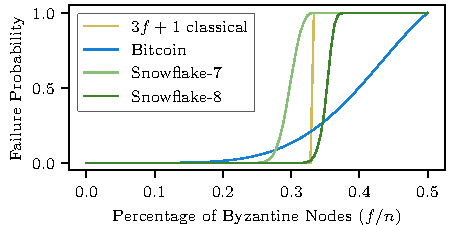
\includegraphics[width=\linewidth]{figures/safety-f-eps.pdf}
%O    \caption{Classical BFT protocols that tolerate $f$ failures will encounter total safety failure when the threshold is exceeded even by one additional node. The Bitcoin curve shows a typical finality choice for Bitcoin where a block is considered final when it is ``buried'' in a branch having 6 additional blocks compared to any other competing forks. Snowflake belongs to the Snow family, and it is configured with $k=10$, $\beta=150$. Snowflake-7,8 uses $\alpha=7$ and $\alpha=8$ respectively (see Section~\ref{sec:protocol} for the definition of $k$, $\alpha$ and $\beta$.}
    \caption{Les protocoles BFT classiques qui tolèrent $f$ défaillances rencontrent une défaillance totale de leur sûreté de fonctionnement quand le seuil est dépassé même d'un seul nœud supplémentaire. La courbe de Bitcoin montre un choix de finalité typique pour Bitcoin où un bloc est considéré final quand il est \guillemotleft\,enterré\,\guillemotright~ dans une branche sous 6 blocs supplémentaires par rapport aux autres branches concurrentes. Snowflake appartient à la famille Snow et est configuré avec $k=10$, $\beta=150$. Snowflake-7,8 utilise $\alpha=7$ et $\alpha=8$ res\-pectivement (voir en section~\ref{sec:protocol} pour la définition de $k$, $\alpha$ et $\beta$.}
    \label{fig:fandepsilon}
\end{figure}

\tronly{%
\begin{figure}[h]
    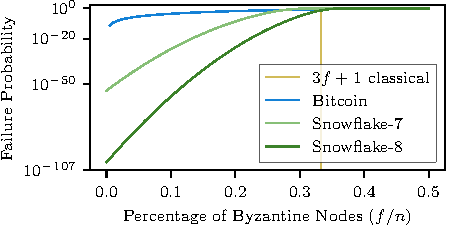
\includegraphics[width=\linewidth]{figures/safety-f-eps-log.pdf}
%O    \caption{Figure~\ref{fig:fandepsilon}, axe des y en log.}
    \caption{Figure~\ref{fig:fandepsilon} avec l'axe des y en log.}
    \label{fig:fandepsilonlog}
\end{figure}
}{}

%O \paragraph{Liveness} All our protocols provide a non-zero probability guarantee of termination within a bounded amount of time. 
\paragraph{Vitalité} Tous nos protocoles fournissent une garantie de probabilité de terminaison dans un laps de temps donné supérieure à zéro.
%O This bounded guarantee is similar to various protocols such as Ben-Or~\cite{ben1983another} and longest-chain protocols.
Cette garantie de limite est similaire à celle de divers protocoles comme Ben-Or~\cite{ben1983another} et les protocoles de chaîne la plus longue.
%O In particular, for Nakamoto consensus, the number of required blocks for a transaction increases exponentially with the number of adversarial nodes, with an asymptote at $f = n/2$ wherein the number is infinite.
En particulier, pour le consensus Nakamoto, le nombre de blocs requis pour une transaction augmente exponentiellement avec le nombre de nœuds antagonistes, avec une asymptote à $f = n/2$ où le nombre est infini. % wut?
%O In other words, the time required for finality approaches $\infty$ as $f$ approaches $n/2$\tronly{ (Figure~\ref{fig:livenessproperties}).}{.}
En d'autres termes, le temps nécessaire à la finalité approche $\infty$ quand $f$ approche $n/2$\tronly{ (figure~\ref{fig:livenessproperties}).}{.}
%O Furthermore, the required number of rounds is calculable ahead of time, as to allow the system designer to tune liveness at the expense of safety. Lastly, unlike traditional consensus protocols and similar to Nakamoto, our protocols benefit from lower adversarial presence, as discussed in property P3 below.
De plus, le nombre requis de tours est calculable à l'avance, ce qui permet au concepteur du système de régler la vitalité aux dépens de la sûreté de fonctionnement. Enfin, contrairement aux protocoles de consensus traditionnels et similairement à Nakamoto, nos protocoles bénéficient d'une moindre présence antagoniste, comme le détaille la propriété P3 ci-dessous.

\tronly{%
\begin{figure}[h!]
    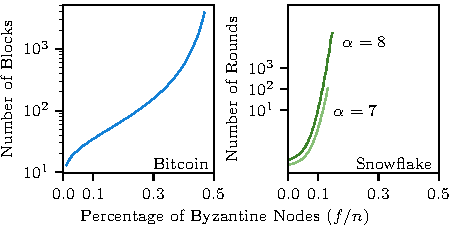
\includegraphics[width=\linewidth]{figures/liveness-f-time.pdf}
%O    \caption{The relation between $f/n$ and the convergence speed, given $\varepsilon = 10^{-20}$. The left figure shows the expected number of blocks to guarantee $\varepsilon$ in Bitcoin, which, counter to commonly accepted folk wisdom, is not a constant $6$, but depends on adversary size to withhold the same $\varepsilon$. The right figure shows the maximum number of rounds required by Snowflake, where being different from Bitcoin, the asymptote is below $0.5$ and varies by the choice of parameters.}
    \caption{Relation entre $f/n$ et la vitesse de convergence pour $\varepsilon = 10^{-20}$. La figure de gauche montre le nombre attendu de blocs pour garantir $\varepsilon$ dans Bitcoin, qui, contrairement à la croyance populaire, n'est pas une constante $6$, mais dépend de la taille de l'adversaire pour maintenir le même $\varepsilon$. La figure de droite montre le nombre maximum de tours requis par Snowflake où, étant différent de Bitcoin, l'asymptote se trouve sous $0.5$ et varie selon les paramètres.}
    \label{fig:livenessproperties}
\end{figure}
}

%O \emph{Formal Guarantees}: Let the system be parameterized for an $\varepsilon$ safety failure probability under a maximum expected $f$ number of adversarial nodes. Let $\Oh{\log n} < t_{max} < \infty$ be the upper bound of the execution of the protocols. The Snow protocols then provide the following guarantees:
\emph{Garantie formelle}\,: Soit un paramétrage du système pour une probabilité de défaillance de la sûreté de fonctionnement $\varepsilon$ pour un nombre maximal attendu $f$ de nœuds antagonistes. Soit $\Oh{\log n} < t_{max} < \infty$ la limite supérieure de l'exécution du protocole. Les protocoles Snow fournissent alors les garanties suivantes\,:
\begin{compactitem}
% RVR: this property is unnecessary because the liveness property already ensures non-triviality
%    \item \textbf{Non-triviality}: To ensure that the protocol carries out real work, decisions must include values proposed by external clients;

%O     \item \textbf{P1. Safety.} When decisions are made by any two correct nodes, they decide on conflicting transactions with negligible probability ($\leq \varepsilon$).
     \item \textbf{P1. Sûreté de fonctionnement.} Quand les décisions sont prises par deux nœuds corrects, ils décident des transactions conflictuelles avec une probabilité négligeable ($\leq \varepsilon$).
    % \item \textbf{P2. Liveness.} Transactions will be accepted by every correct node in $\Oh{\log n}$ rounds if either the observed Byzantine presence $f'$, where $f' < f$, is sufficiently small, or the network is initialized in a univalent state.
%O     \item \textbf{P2. Liveness (Upper Bound).} Snow protocols terminate with a strictly positive probability within $t_{max}$ rounds.  
     \item \textbf{P2. Vitalité (limite supérieure).} Les protocoles Snow se terminent avec une probabilité strictement positive en au plus $t_{max}$ tours.
%O     \item \textbf{P3. Liveness (Strong Form).} If $f \leq \Oh{\sqrt{n}}$, then the Snow protocols terminate with high probability ($\geq 1 - \varepsilon$) in $\Oh{\log{n}}$ rounds. 
     \item \textbf{P3. Vitalité (forme forte).} Si $f \leq \Oh{\sqrt{n}}$, alors les protocoles Snow se terminent avec une forte probabilité ($\geq 1 - \varepsilon$) en $\Oh{\log{n}}$ tours.
\end{compactitem}
% Instead of unconditional agreement, our approach guarantees that safety will be upheld with probability $1-\varepsilon$, where the choice of the security parameter $\varepsilon$ is under the control of the system designer and applications.

%O \paragraph{Network} 
\paragraph{Réseau} 
%O In the standard definition of asynchrony~\cite{ben1983another}, message transmission time is finite, but the distribution is unspecified (and thus the delivery time can be unbounded for some messages). This implies that the scheduling of message transmission itself could behave arbitrarily, and potentially even maliciously (with full asynchrony).
Dans la définition standard de l'asynchronie~\cite{ben1983another}, le temps de transmission des messages est fini, mais la distribution n'est pas spécifiée (donc le temps de délivrance peut être non borné pour certains messages). Cela implique que l'ordonnancement de la transmission des messages lui-même peut être quelconque, voire potentiellement malveillant (pour une complète asynchronie).
%O We use a modified version of this model, which is well-accepted~\cite{banerjee2014epidemic, ganesh2005effect, draief2006thresholds, keeling2011modeling, liggett1997stochastic} in the analysis of epidemic networks and gossip-based stochastic systems. In particular, we fix the distribution of message delay to that of the exponential distribution.
Nous employons une version mo\-difiée de ce modèle, lequel est bien accepté~\cite{banerjee2014epidemic, ganesh2005effect, draief2006thresholds, keeling2011modeling, liggett1997stochastic} dans l'analyse des réseaux épidémiques et des systèmes stochastiques à base de \emph{gossip}. En particulier, nous fixons la distribution des délais de messages à celle de la distribution exponentielle.
%O We note that, just like in the standard asynchronous model, there is a strictly non-zero probability that any correct node may execute its next local round only after an arbitrarily large amount of time has passed.
Nous notons que, tout comme dans le modèle asynchrone standard, il existe une probabilité strictement non-nulle que tout nœud correct ne peut exécuter son prochain tour local qu'après qu'un laps de temps arbitrairement long a passé.
%O Furthermore, we also note that scheduling only applies to correct nodes, and the adversary may execute arbitrarily, as discussed later. 
De plus, notons également que l'ordonnancement ne s'applique qu'aux nœuds corrects, et que l'adversaire peut s'exécuter arbitrairement, comme nous le verrons plus loin.

%O \paragraph{Achieving Liveness}
\paragraph{Objectifs de vitalité}
%O Classical consensus that works with asynchrony does not get stuck in a single phase of voting because the vote initiator always polls votes from all known participants and waits for $n - f$ responses.
Les consensus classiques qui fonctionnent en asynchronie ne restent pas bloqués lors d'une phase de vote car l'initiateur du vote interroge toujours tous les participants connus et attend $n - f$ réponses.
%The consequence of these two assumptions is therefore that progress cannot be indefinitely delayed by the adversary since the correct nodes (whose number is sufficient for voting) will eventually deliver the required messages.
%O In our system, however, nodes operate via subsampling, hence it is possible for a single sample to select a majority of adversarial nodes, and therefore the node gets stuck waiting for the responses. To ensure liveness, a node should be able to wait with some timeout. Therefore, our protocols are synchronous in order to guarantee liveness. Lastly, it is worth noting that Nakamoto consensus is synchronous, in which the required difficulty of proof-of-work is dependent on the maximum network delay~\cite{PassSS17}. %Also, other protocols that rely on gossip [Citation here] are also essentially synchronous due to the synchronous nature of gossip protocols. \editinsert{RvR pointed this out, we need to carefully word it though.
Dans notre système, cependant, les nœuds opèrent par sous-échantillonnage, d'où la possibilité pour un seul échantillon qu'une majorité de nœuds antagonistes soit sélectionné, ce qui contraint le nœud à attendre en vain une réponse. Pour s'assurer de la vitalité, un nœud doit pouvoir limiter son attente. Enfin, il faut noter que le consensus Nakamoto est synchrone et que la difficulté requise pour la preuve de travail dépend du délai maximum du réseau~\cite{PassSS17}. 

%O \paragraph{Adversary}
\paragraph{Adversité}
%O The adversarial nodes execute under their own internal scheduler, which is unbounded in speed, meaning that all adversarial nodes can execute at any infinitesimally small point in time, unlike correct nodes. 
Les nœuds antagonistes s'exécutent avec un ordonnanceur interne qui leur est propre, non limité en vitesse, ce qui signifie que tout nœud antagoniste peut s'exécuter à un moment précis infiniment petit, au contraire des nœuds corrects.
%O The adversary can view the state of every honest node at all times and can instantly modify the state of all adversarial nodes. 
L'adversaire peut voir l'état de chaque nœud correct à tout moment et peut instantanément modifier l'état de tout nœud antagoniste.
%O It cannot, however, schedule or modify communication between correct nodes.
Il ne peut, cependant, ordonnancer ou modifier la communication entre les nœuds corrects.
%O Finally, we make zero assumptions about the behavior of the adversary, meaning that it can choose any execution strategy of its liking.
Enfin, nous ne faisons aucune hypothèse sur le comportement de l'adversaire, ce qui signifie qu'il peut choisir la stratégie d'exécution qui lui convient.
%O In short, the adversary is computationally bounded (it cannot forge digital signatures) but otherwise is point-to-point informationally unbounded (knows all state) and round-adaptive (can modify its strategy at any time). 
En résumé, l'adversaire est limité en puissance informatique (il ne peut pas forger des signatures numériques) mais, hormis cela, il n'est pas limité en matière informationnelle (il connaît tout de l'état) et il est adaptatif en matière de tours (il peut modifier sa stratégie à tout moment).

\paragraph{Attaques Sybil}
%O Consensus protocols provide their guarantees based on assumptions that only a fraction of participants are adversarial.
Les protocoles de consensus fournissent leurs garanties en se fondant sur l'hypothèse que seule une fraction des participants sont antagonistes.
%O These bounds could be violated if the network is naively left open to arbitrary participants.
Ces limites peuvent être violées si le réseau est naïvement laissé ouvert à des parti\-cipants quelconques.
%O In particular, a Sybil attack~\cite{douceur2002sybil}, wherein a large number of identities are generated by an adversary, could be used to exceed the bounds.
En particulier, une attaque Sybil~\cite{douceur2002sybil}, où un grand nombre d'identités sont générées par un adversaire, peut être employée pour dépasser ces limites.

%O A long line of work, including PBFT~\cite{castro1999practical}, treats the Sybil problem separately from consensus, and rightfully so, as Sybil control mechanisms are distinct from the underlying, more complex agreement protocol\footnote{This is not to imply that every consensus protocol can be coupled/decoupled with every Sybil control mechanism.}.
Une longue suite de travaux, comme PBFT~\cite{castro1999practical}, sépare le problème de Sybil de celui du consensus, à juste titre puisque les mécanismes de contrôle de Sybil sont distincts du protocole d'accord plus complexe sous-jacent\footnote{Cela n'implique pas que tout protocole de consensus puisse être couplé ou découplé de tout mécanisme de contrôle de Sybil.}.
%O In fact, to our knowledge, only Nakamoto-style consensus has ``baked-in'' Sybil prevention as part of its consensus, made possible by chained proof-of-work~\cite{aspnes2005exposing}, which requires miners to continuously stake a hardware investment.
En fait, à notre connaissance, le consensus Nakamoto est le seul à avoir intégré la protection anti-Sybil dans son consensus, chose rendue possible par la preuve de travail chaînée~\cite{aspnes2005exposing} qui demande aux mineurs de continuellement mettre en jeu un investissement matériel.
%O Other protocols, discussed in Section~\ref{sec:related-work}, rely on proof-of-stake (by economic argument) or proof-of-authority (by administrative argument that makes the system ``permissioned'').
D'autres protocoles, dont il est question en section~\ref{sec:related-work}, se basent sur la preuve d'enjeu (\emph{proof of stake} ou PoS, par un argument économique) ou la preuve d'autorité (\emph{proof of authority} ou PoA, par un argument administratif) qui rend le système \guillemotleft\,permissionné\,\guillemotright.
%O The consensus protocols presented in this paper can adopt any
%O Sybil control mechanism, although proof-of-stake is most aligned with their quiescent operation.
Les protocoles de consensus présentés dans cet article peuvent adopter n'importe quel mécanisme de contrôle de Sybil, bien que la preuve d'enjeu soit la plus en ligne avec le caractère économe de leur opération.
%O One can use an already established proof-of-stake based mechanism~\cite{GiladHMVZ17}.
On peut utiliser un mécanisme en preuve d'enjeu déjà établi.
%O The full deployment of an autonomous P2P payment system incorporating staking mechanism is beyond the scope of this paper, whose focus is on a novel design paradigm of the core consensus algorithm.
Le déploiement complet d'un système de paiement autonome en P2P incorporant des mécanismes d'enjeu dépasse le cadre de cet article, dont l'objet est un nouveau paradigme de conception de l'algorithme de consensus.

% Sybil control mechanisms are orthogonal and separate from the consensus protocols. All such protocols, excluding Nakamoto-style consensus protocols, require a mechanism for network identity establishment. In a real implementation of Avalanche, the Sybil problem would be solved through a staking mechanism. 

%O \paragraph{Flooding Attacks}
\paragraph{Attaques par inondation}
%O Flooding/spam attacks are a problem for any distributed system. 
Les attaques par inondation et par spam représentent un problème pour tout système distribué.
%O Without a protection mechanism, an attacker can generate large numbers of transactions and flood protocol data structures, consuming storage.
Sans mécanisme de protection, un attaquant peut générer un grand nombre de transactions et inonder les structures de données du protocole, consommant ainsi des ressources de stockage.
% Although there is no proper, protocol-level methodology to prevent such an attack, there are very effective heuristics that we can employ.
%O There are a multitude of techniques to deter such attacks, including network-layer protection, proof-of-authority, local proof-of-work and economic mechanisms. 
Il existe une multitude de techniques pour repousser ces attaques comme la protection de la couche réseau, la preuve d'autorité, la preuve de travail local, ainsi que des mécanismes économiques.
%O In Avalanche, we use transaction fees, making such attacks costly even if the attacker is sending money back to addresses under its control.
Dans Avalanche, nous utilisons les frais de transaction, rendant ainsi ces attaques coûteuses même si l'attaquant renvoie l'argent aux adresses qu'il contrôle.



%O \paragraph{Additional Assumptions}
\paragraph{Hypothèses supplémentaires}
%O We do not assume that all members of the network are known to all participants, but rather may temporarily have some discrepancies in network view.
Nous ne supposons pas que tous les membres du réseau sont connus de tous les participants, car la vue du réseau qu'ont ces derniers peut souffrir d'incohérences temporaires.
%O We quantify the bounds on the discrepancy in Appendix~\ref{sec:full-analysis-churn}.
Nous en quantifions les bornes en annexe~\ref{sec:full-analysis-churn}.
%O We assume a safe bootstrapping mechanism, similar to that of Bitcoin, that enables a node to connect with sufficiently many correct nodes to acquire a statistically unbiased view of the network.
Nous supposons un mécanisme de démarrage initial sûr, similaire à celui de Bitcoin, qui permet à un nœud de se connecter à suffisamment de nœuds corrects pour acquérir une vue statistiquement non biaisée du réseau.
%O We do not assume a PKI\@.
Nous ne prévoyons pas une PKI\@.
%O Finally, we make standard cryptographic assumptions related to digital signatures and hash functions.
Enfin, nous nous reposons sur les hypothèses standard en matière de cryptographie dans le domaine des signatures numériques et des fonctions de hachage.
%\editinsert{TODO: Talk about synchrony assumption, and justify it by mentioning Bitcoin.}
%\editinsert{TODO: Talk about we don't address Sybil attack, and justify it by mentioning Algorand (we also use Algorand as a comparison in Evaluation, so it will totally make sense here.}


\section{Conception du Protocole}\label{sec:protocol}
Nous partons d'un protocole non résistant au problème des généraux byzantins appelé Slush, en amenant
progressivement Snowflake et Snowball, tous basés sur le même mécanisme métastable de vote basé sur une majorité.
Ces derniers sont des protocoles de consensus à simple décret présentant plusieurs niveaux de robustesse. Nous
détaillons les caractéristiques complètes de ces protocoles dans cette section, suivie de leur analyse en section
suivante, les preuves formelles étant disponibles en annexe.

%O \section{Protocol Design}\label{sec:protocol}
%O We start with a non-BFT protocol called Slush and progressively build up to Snowflake and Snowball, all based on the same common majority-based metastable voting mechanism.
%O These protocols are single-decree consensus protocols of increasing robustness.
%O We provide full specifications for the protocols in this section, and defer the analysis to the next section, and present formal proofs in the appendix.

%0 \subsection{Slush: Introducing Metastability}
\subsection{Slush\,: présentation de la métastabililté}

%O The core of our approach is a single-decree consensus protocol,
%O inspired by epidemic or gossip protocols.
%O The simplest protocol, Slush, is the foundation of this family, shown in Figure~\ref{fig:slush-loop}.
%O Slush is \emph{not} tolerant to Byzantine faults, only crash-faults (CFT), but serves as an illustration for the BFT protocols that follow.
%O For ease of exposition, we will describe the operation of Slush using a decision between two conflicting colors, red and blue.

Le principe de notre approche est un protocole de consensus à simple décret inspiré des protocoles dits épidémiques
ou \emph{gossip}. Le protocole le plus simple, Slush, est la fondation de cette famille, comme le montre la
figure~\ref{fig:slush-loop}. Slush \emph{n'est pas} tolérant aux fautes byzantines, seulement aux défauts
de fonctionnement (CFT), mais sert à mettre en avant les autres protocoles tolérants aux fautes byzantines qui vont
suivre. Dans un souci de simplicité de présentation, nous décrirons le fonctionnement de Slush en le comparant
à une décision à prendre entre deux couleurs incompatibles, le rouge et le bleu.

%O In Slush, a node starts out initially in an uncolored state.
%O Upon receiving a transaction from a client, an uncolored node updates its own color to the one carried in the transaction and initiates a query.
%O To perform a query, a node picks a small, constant sized ($k$) sample of the network uniformly at random, and sends a query message.
%O Upon receiving a query, an uncolored node adopts the color in the query, responds with that color, and initiates its own query, whereas a colored node simply responds with its current color.
%O Once the querying node collects $k$ responses, it checks if a fraction $\ge\alpha$ are for the same color, where $\alpha > \floor{k/2}$ is a protocol parameter.
%O If the $\alpha$ threshold is met and the sampled color differs from the node's own color, the node flips to that color.
%O It then goes back to the query step, and initiates a subsequent round of query, for a total of $m$ rounds.
%O Finally, the node decides the color it ended up with at time $m$.

Avec Slush, un nœud démarre dans un état de couleur neutre. Après réception d'une transaction envoyée par un client,
un nœud de couleur neutre adopte la couleur définie dans la transaction et initie une requête. Pour lancer une
requête, le nœud choisit un échantillon réduit et de taille constante ($k$) de nœuds appartenant au réseau suivant
une distribution uniformément aléatoire puis initie sa propre requête, tandis qu'un nœud déja coloré répond
simplement avec sa couleur actuelle. Une fois que le nœud qui fait la requête récupère $k$ réponses, il vérifie si
une proportion $\ge\alpha$ de l'échantillon retourne la même couleur, $\alpha > \floor{k/2}$ étant un paramètre
du protocole. Si le seuil $\alpha$ est dépassé et que la couleur dominante revenant de l'échantillon sollicité est
différente de la couleur propre du nœud à l'origine de la requête, ce nœud adopte cette nouvelle couleur. Il revient
ensuite à l'étape de génération de la requête et lance un nouveau tour de requête jusqu'à un total de $m$ tours.
En définitive, le nœud décide de sa couleur finale à l'instant $m$.

\algnewcommand{\IIf}[1]{\State\algorithmicif\ #1\ \algorithmicthen}
\algnewcommand{\EndIIf}{\unskip\ \algorithmicend\ \algorithmicif}

\newcommand{\codecolor}{\mathit{col}}
\newcommand{\codecount}{\mathit{cnt}}
\newcommand{\codelastcol}{\mathit{lastcol}}
\newcommand{\assign}{\coloneqq}
\begin{figure}
    \small
\begin{algorithmic}[1]
    \Procedure{onQuery}{$v, \codecolor'$}
        \IIf{$\codecolor = \bot$} $\codecolor \assign \codecolor'$
        \State\Call{répondre}{$v, \codecolor$}
    \EndProcedure
    \Procedure{slushLoop}{$u, \codecolor_0 \in \{\texttt{R}, \texttt{B}, \bot\}$}
        \State $\codecolor \assign \codecolor_0$ \textrm{// initialise avec une couleur}
        \For{$r \in \{1\ldots m\}$}
            \State \textrm{// Si $\bot$, saute jusqu'à ce que \textsc{onQuery} applique la couleur}
            \If{$\codecolor = \bot$}
                \Continue
            \EndIf
            \State \textrm{// échantillonne aléatoirement parmi les nœuds connus}
            \State $\mathcal{K} \assign \Call{échantillon}{\mathcal{N}\backslash u, k}$
            \State $P \assign \texttt{[}\Call{requête}{v, \codecolor}\quad\textbf{pour}\ v \in \mathcal{K}\texttt{]}$
            \For{$\codecolor' \in \{\texttt{R}, \texttt{B}\}$}
                \If{$P.\Call{nombre}{\codecolor'} \ge \alpha$}
                    \State $\codecolor \assign \codecolor'$
                \EndIf
            \EndFor
        \EndFor
        \State \Call{accepte}{$\codecolor$}
    \EndProcedure
    \captionof{figure}{Protocole Slush. Temps d'expiration omis dans un souci de lisibilité.}\label{fig:slush-loop}
\end{algorithmic}
\end{figure}

%O Slush has a few properties of interest.
%O First, it is almost \emph{memoryless}: a node retains no state between rounds other than its current color, and in particular maintains no history of interactions with other peers.
%O Second, unlike traditional consensus protocols that query every participant, every round involves sampling just a small, constant-sized slice of the network at random.
%O Third, Slush makes progress under any network configuration (even fully bivalent state, i.e. 50/50 split between colors), since random perturbations in sampling will cause one color to gain a slight edge and repeated samplings afterwards will build upon and amplify that imbalance.
%O Finally, if $m$ is chosen high enough, Slush ensures that all nodes will be colored identically with high probability (whp).
%O Each node has a constant, predictable communication overhead per round, and $m$ grows logarithmically with $n$.

Slush possède quelques propriétés intéressantes. Premièrement, il n'a quasiment \emph{pas besoin de mémoire}\,: un nœud ne
stocke aucun état intermédiaire entre chaque tour autre que sa couleur actuelle, et plus particulièrement ne stocke
aucun historique de ses interactions avec les autres nœuds. Deuxièmement, contrairement aux protocoles de consensus
traditionnels qui sollicitent tous les participants, chaque tour n'implique qu'un échantillon du réseau réduit et de
taille constante choisi aléatoirement. Troisièmement, Slush progresse quelque soit la configuration du réseau (même
depuis un état entièrement bivalent, c'est-à-dire un partage 50/50 entre les deux couleurs) puisque des perturbations aléatoires
sur l'échantillonnage auront pour conséquence de fournir un léger avantage à l'une des deux couleurs, lequel sera ensuite
amplifié au fur et à mesure des échantillonnages.
Finalement, si $m$ est choisi pour être suffisamment élevé, Slush s'assure que tous les nœuds convergent vers la
même couleur avec une forte probabilité. Chaque nœud nécessite un nombre de communications par tour constant et
prévisible, et $m$ croît de manière logarithmique suivant $n$.

\tronly{
%O The Slush protocol does not provide a strong safety guarantee in the presence of Byzantine nodes.
%O In particular, if the correct nodes develop a preference for one color, a Byzantine adversary can attempt to flip nodes
%O to the opposite so as to keep the network in balance, preventing a decision.
%O We address this in our first BFT protocol that introduces more state storage at the nodes.

Le protocole Slush ne fournit pas de fortes garanties quant à la sûreté de fonctionnement en présence de nœuds
byzantins. En particulier, si les nœuds légitimes développent une préférence pour une certaine couleur, un adversaire
byzantin pourra inverser la couleur des nœuds afin de maintenir le système à l'équilibre, empêchant ainsi de prendre une
décision. Nous étudions ce problème dans notre premier protocole BFT qui ajoute un stockage de l'état sur les nœuds.
}{
%O We next examine how to extend Slush to tolerate Byzantine behavior.
Nous examinons ensuite la manière de fournir à Slush une tolérance aux comporements byzantins.
}

\subsection{Snowflake\,: BFT}

Snowflake améliore Slush en ajoutant un compteur unique qui reflète la force de conviction d'un nœud concernant sa couleur
actuelle. Ce compteur associé à chaque nœud stocke le nombre d'échantillons du réseau consécutifs que le nœud a
sollicité et qui ont retourné la même couleur. Un nœud accepte la couleur actuelle lorsque son compteur atteint $\beta$,
un autre paramètre de sécurité. La figure~\ref{fig:snowflake-loop} montre le protocole amélioré qui inclut les
modifications suivantes\,:

%O Snowflake augments Slush with a single counter that captures the strength of a node's conviction in its current color.
%O This per-node counter stores how many consecutive samples of the network by that node have all yielded the same color.
%O A node accepts the current color when its counter reaches $\beta$, another security parameter.
%O Figure~\ref{fig:snowflake-loop} shows the amended protocol, which includes
%O the following modifications:

\begin{compactenum}
	\item Chaque nœud maintient un compteur $\mathit{cnt}$\,;
    \item À chaque changement de couleur, le compteur $\mathit{cnt}$ se réinitialise à 0\,;
    \item Après chaque requête réussie qui renvoie $\ge \alpha$ réponses en faveur de la même couleur que le nœud,
      ce dernier incrémente $\mathit{cnt}$.
\end{compactenum}

%O \begin{compactenum}
%O 	\item Each node maintains a counter $\mathit{cnt}$;
%O     \item Upon every color change, the node resets $\mathit{cnt}$ to 0;
%O     \item Upon every successful query that yields $\ge \alpha$ responses for the same color as the node, the node increments $\mathit{cnt}$.
%O \end{compactenum}

\newcommand{\codemaj}{\mathit{maj}}
\newcommand{\codefalse}{\texttt{false}}
\newcommand{\codetrue}{\texttt{true}}
\begin{figure}
    \small
\begin{algorithmic}[1]
    \Procedure{snowflakeLoop}{$u, \codecolor_0 \in \{\texttt{R}, \texttt{B}, \bot\}$}
        \State $\codecolor \assign \codecolor_0$, $\codecount \assign 0$
        \While{\textrm{undecided}}
            \If{$\codecolor = \bot$}
                \Continue
            \EndIf
            \State $\mathcal{K} \assign \Call{sample}{\mathcal{N}\backslash u, k}$
            \State $P \assign \texttt{[}\Call{query}{v, \codecolor}\quad\textbf{for}\ v \in \mathcal{K}\texttt{]}$
            \State $\codemaj \assign \codefalse$
            \For{$\codecolor' \in \{\texttt{R}, \texttt{B}\}$}
            \If{$P.\Call{count}{\codecolor'} \ge \alpha$}
                \State $\codemaj \assign \codetrue$
                \If{$\codecolor' \neq \codecolor$}
                    \State $\codecolor \assign \codecolor'$, $\codecount \assign 1$
                \Else\hspace{1ex}$\codecount\texttt{++}$
                \EndIf
                \IIf {$\codecount \ge \beta$} \Call{accept}{$\codecolor'$}
            \EndIf
            \EndFor
            \IIf{$\codemaj = \codefalse$} $\codecount \assign 0$
        \EndWhile
    \EndProcedure
    \captionof{figure}{Snowflake.}\label{fig:snowflake-loop}
\end{algorithmic}
\end{figure}

\begin{figure}[t]
    \small
\begin{algorithmic}[1]
    \Procedure{snowballLoop}{$u, \codecolor_0 \in \{\texttt{R}, \texttt{B}, \bot\}$}
        \State $\codecolor \assign \codecolor_0$, $\codelastcol \assign \codecolor_0$, $\codecount \assign 0$
        \State $d[\texttt{R}] \assign 0$, $d[\texttt{B}] \assign 0$
        \While{\textrm{undecided}}
            \IIf{$\codecolor = \bot$} \Continue
            \State $\mathcal{K} \assign \Call{sample}{\mathcal{N}\backslash u, k}$
            \State $P \assign \texttt{[}\Call{query}{v, \codecolor}\quad\textbf{for}\ v \in \mathcal{K}\texttt{]}$
            \State $\codemaj \assign \codefalse$
            \For{$\codecolor' \in \{\texttt{R}, \texttt{B}\}$}
            \If{$P.\Call{count}{\codecolor'} \ge \alpha$}
                \State $\codemaj \assign \codetrue$
                \State $d[\codecolor']\texttt{++}$
                \If {$d[\codecolor'] > d[\codecolor]$}
                        \State$\codecolor \assign \codecolor'$
                \EndIf
                \If{$\codecolor' \neq \codelastcol$}
                    \State$\codelastcol \assign \codecolor'$, $\codecount \assign 1$
                \Else\hspace{1ex}$\codecount\texttt{++}$
                \EndIf
                \IIf {$\codecount \ge \beta$} \Call{accept}{$\codecolor'$}
            \EndIf
            \EndFor
            \IIf{$\codemaj = \codefalse$} $\codecount \assign 0$
        \EndWhile
    \EndProcedure
    \captionof{figure}{Snowball.}\label{fig:snowball-loop}
\end{algorithmic}
\end{figure}

Quand le protocole est correctement paramétré pour un seuil donné de nœuds byzantins et un niveau de garantie
$\varepsilon$, il peut garantir à la fois la sécurité de fonctionnement (P1) et la vitalité (P2, P3).
Comme nous le démontrons plus loin, il existe un état irréversible à partir duquel une décision est inévitable. Les nœuds
légitimes commencent à se positionner après cet état irréversible et adoptent la même couleur. Une intuition
supplémentaire, que nous ne détaillerons pas dans ce papier, indique l'existence d'un point de changement de phase à
partir duquel les nœuds byzantins perdent toute capacité à maintenir le réseau dans un état bivalent.

%O When the protocol is correctly parameterized for a given threshold of Byzantine nodes and a desired $\varepsilon$-guarantee, it can ensure both safety (P1) and liveness (P2, P3).
%O As we later show, there exists an irreversible state after which a decision is inevitable. Correct nodes begin to commit past the irreversible state to adopt the same color, whp. For additional intuition, which we do not expand in this paper, there also exists a phase-shift point, where the Byzantine nodes lose ability to keep network in a bivalent state.

%O \subsection{Snowball: Adding Confidence}

\subsection{Snowball\,: ajout de la confiance}

La notion d'état de Snowflake est éphémère\,: le compteur est réinitialisé à chaque changement de couleur.
Snowball améliore Snowflake avec des \emph{compteurs de confiance} qui reflètent le nombre de requêtes ayant renvoyé
un résultat en faveur de la couleur du nœud au dessus d'un certain seuil (figure ~\ref{fig:snowball-loop}).
Un nœud prend une décision s'il obtient $\beta$ réponses consécutives en faveur d'une couleur. Cependant, il change
sa préférence uniquement sur la base de la confiance totale accumulée. Les différences entre Snowflake et Snowball
sont les suivantes\,:

\begin{compactenum}
    \item Après chaque requête réussie, le nœud incrémente son compteur de confiance associé à la couleur retournée\,;
    \item Un nœud change de couleur quand la confiance associée à sa couleur actuelle devient inférieure à la
      valeur de la confiance associée à la nouvelle couleur.
\end{compactenum}

%O Snowflake's notion of state is ephemeral: the counter gets reset with every color flip.
%O Snowball augments Snowflake with \emph{confidence counters} that capture the number of queries that have yielded a threshold result for their corresponding color (Figure ~\ref{fig:snowball-loop}).
%O A node decides if it gets $\beta$ consecutive chits for a color. However, it only changes preference based on the total accrued confidence.
%O The differences between Snowflake and Snowball are as follows:
%O \begin{compactenum}
%O     \item Upon every successful query, the node increments its confidence counter for that color.
%O     \item A node switches colors when the confidence in its current color becomes lower than the confidence value of the new color.
%O \end{compactenum}


\section{Analyse}
\label{sec:analysis}
Pour des raisons de manque de place, nous déplaçons certains détails importants vers l'annexe~\ref{sec:full-analysis},
dans laquelle nous démontrons que sous certaines hypothèses distinctes et indépendantes, la famille de protocoles de
consensus Snow possède des propriétés de sûreté de fonctionnement (P1) et de vitalité (P2, P3). Dans cette section,
nous résumons nos résultats principaux en fournissant des ébauches de preuves.

%O \section{Analysis}
%O \label{sec:analysis}
%O Due to space limits, we move some core details to Appendix~\ref{sec:full-analysis}, where we show that under certain independent and distinct assumptions, the Snow family of consensus protocols provide safety (P1) and liveness (P2, P3) properties.
%O In this section, we summarize our core results and provide some proof sketches.

\paragraph{Notation} En considérant que le réseau consiste en un ensemble de $n$ nœuds (représentés par l'ensemble
$\mathcal{N}$), où $c$ sont des nœuds légitimes (représentés par l'ensemble $\mathcal{C}$) et $f$ sont les nœuds
byzantins (représentés par l'ensemble $\mathcal{B}$). Soient $u, v \in \mathcal{C}$ des références à deux nœuds
légitimes pris au hasard dans le réseau. Soient $k, \alpha, \beta \in \mathbb{Z}^+$ des entiers positifs où
$\alpha > \floor{k/2}$. A partir de maintenant, $k$ fera toujours référence à la taille des déchantillons du réseau,
où $k \leq n$, et $\alpha$ sera le seuil de majorité requis pour considérer l'expérience de vote comme «\,réussie\,».
En général, nous définissons $\mathcal{S}$ comme étant l'état (ou la configuration) du réseau à tout moment.

%O \paragraph{Notation} Let the network consist of a set of $n$ nodes (represented by set $\mathcal{N}$), where $c$ are correct nodes (represented by set $\mathcal{C}$) and $f$ are Byzantine nodes (represented by set $\mathcal{B}$).
%O Let $u, v \in \mathcal{C}$ refer to any two correct nodes in the network. Let $k, \alpha, \beta \in \mathbb{Z}^+$ be positive integers where $\alpha > \floor{k/2}$. From now on, $k$ will always refer to the network sample size, where $k \leq n$, and $\alpha$ will be the majority threshold required to consider the voting experiment a ``success''. In general, we will refer to $\mathcal{S}$ as the state (or configuration) of the network at any given time.
%O

\paragraph{Framework de modélisation} Afin de modéliser nos protocoles de manière formelle, nous utilisons des
processus de Markov à temps continu (CTMC). L'espace contenant les états est dénombrable (et fini), et les transitions
entre états s'opèrent sur un espace de temps continu. Les CTMC proposent une modélisation naturelle de nos protocoles
sachant que les transitions entre états ne se font pas par étapes et en marche ordonnée pour chaque nœud (à la fin de
chaque unité de temps) mais arrivent plutôt à n'importe quel moment et indépendamment des autres nœuds.

Nous concentrons l'étude sur un consensus binaire, même si les résultats en termes de sûreté de fonctionnement se
généralisent pour plus de deux valeurs. Nous pouvons imaginer le réseau comme un ensemble de nœuds colorés, soit en
rouge, soit en bleu, et nous ferons référence à cette configuration à l'instant $t$ comme étant $\mathcal{S}_t$.
Nous modélisons nos protocoles à travers un processus à temps continu contenant deux états, dans lequel tous les nœuds
sont rouges ou tous les nœuds sont bleus. L'espace $\mathcal{S}$ des états du processus stochastique est une version
condensée de l'espace de configuration complet, où chaque état $\{0, \dots, n\}$ représente le nombre total de nœuds
bleus dans le système.

La simplification qui nous permet d'analyser ce système consiste à s'affranchir du besoin de garder un historique de
tous les chemins d'exécution, ainsi que de toutes les stratégies d'attaque possibles, et de se concentrer 
entièrement sur un unique état quelle que soit la manière d'arriver à celui-ci. Plus spécifiquement, l'idée principale
à retenir de notre analyse est l'identification d'un état \textit{d'irréversibilité} du système, cet état à partir
duquel un tel nombre de nœuds légitimes a adopté soit la couleur rouge soit la couleur bleue que la probabilité de
revenir à la couleur minoritaire est très faible.

%O \paragraph{Modelling Framework} To formally model our protocols, we use continuous-time Markov processes (CTMC).
%O The state space is enumerable (and finite), and state transitions occur in continuous time.
%O CTMCs naturally model our protocols since state transitions do not occur in epochs and in lockstep for every node (at the end of every time unit) but rather occur at any time and independently of each other.

%O We focus on binary consensus, although the safety results generalize to more than two values. We can think of the network as a set of nodes either colored red or blue, and we will refer to this configuration at time $t$ as $\mathcal{S}_t$.
%O We model our protocols through a continuous-time process with two absorbing states, where either all nodes are red or all nodes are blue.
%O The state space $\mathcal{S}$ of the stochastic process is a condensed version of the full configuration space, where each state $\{0, \dots, n\}$ represents the total number of blue nodes in the system.

%O The simplification that allows us to analyze this system is to obviate the need to keep track of all of the execution paths, as well as all possible adversarial strategies, and rather focus entirely on a single state of interest, without regards to how we achieve this state.
%O More specifically, the core extractable insight of our analysis is in identifying the \textit{irreversibility} state of the system, the state upon which so many correct nodes have usurped either red or blue that reverting back to the minority color is highly unlikely.

\subsection{Sûreté de fonctionnement}

%O \subsection{Safety}

\paragraph{Slush}
Nous partons du principe que tous les nœuds partagent le même $\mathcal{N}$, et 
nous expliquons en annexe~\ref{sec:full-analysis-churn} comment assouplir l'exigence de la connaissance des participants.
Nous modélisons la dynamique du système grâce à un processus à temps continu contenant deux états, tous les nœuds étant
rouges ou tous les nœuds étant bleus. Soit $\{X_{t \geq 0}\}$ la variable aléatoire qui décrit l'état du système à
l'instant $t$, où $X_0 \in \{0, \dots, c\}$.
Nous commençons par détailler le résultat le plus important de la dynamique de la sûreté de fonctionnement de notre
processus\,: les probabilités de \emph{réversibilité} du processus \textbf{Slush}. Tous les autres résultats formels de
ce papier sont, en simplifiant, des dérivations et améliorations intuitives de ce résultat.

%0 \paragraph{Slush}
%0 We assume that
%0 %$\mathcal{L}(u) = \mathcal{N}$ for all $u \in \mathcal{N}$.
%0 all nodes share the same $\mathcal{N}$, and in
%0 Appendix~\ref{sec:full-analysis-churn}, we sketch how to relax the requirement of the membership knowledge.
%0 We model the dynamics of the system through a continuous-time process where two states are absorbing, namely the all-red or all-blue state. Let $\{X_{t \geq 0}\}$ be the random variable that describes the state of the system at time $t$, where $X_0 \in \{0, \dots, c\}$.
%0 We begin by immediately discussing the most important result of the safety dynamics of our processes: the \emph{reversibility} probabilities of the \textbf{Slush} process. All the other formal results in this paper are, informally speaking, intuitive derivations and augmentations of this result.

\begin{theorem}
Prenons la configuration du système à l'instant $t$ comme étant $\mathcal{S}_t = n/2 + \delta$, ce qui signifie que le
réseau a dérivé de $2\delta$ nœuds bleus de plus que les nœuds rouges ($\delta = 0$ signifie que rouges et bleus
sont en nombre égal). $\xi_\delta$ étant la probabilité d'un basculement vers l'état où tous les nœuds sont rouges,
nous avons donc pour tout $0 \leq \delta \leq n/2$
\begin{equation}
\begin{split}
    \xi_\delta &\leq \left(\dfrac{1/2 - \delta/n}{\alpha/k}\right)^{\alpha}\left(\dfrac{1/2 + \delta/n}{1- \alpha/k}\right)^{k-\alpha}\\
    &\leq e^{-2((\alpha/k) - (1/2) + (\delta/n))^2 k}
\end{split}
\end{equation}
\end{theorem}

\begin{proof}
Cette borne suit les bornes de queue dérivées de Hoeffding de la distribution hypergéométrique définie par
Chvatal~\cite{chvatal1979tail}.
\end{proof}

%O \begin{theorem}
%O Let the configuration of the system at time $t$ be $\mathcal{S}_t = n/2 + \delta$, meaning that the network has drifted to $2\delta$ more blue nodes than red nodes ($\delta = 0$ means that red and blue are equal). Let $\xi_\delta$ be the probability of absorption to the all-red state (minority). Then, for all $0 \leq \delta \leq n/2$, we have
%O \begin{equation}
%O \begin{split}
%O     \xi_\delta &\leq \left(\dfrac{1/2 - \delta/n}{\alpha/k}\right)^{\alpha}\left(\dfrac{1/2 + \delta/n}{1- \alpha/k}\right)^{k-\alpha}\\
%O     &\leq e^{-2((\alpha/k) - (1/2) + (\delta/n))^2 k}
%O \end{split}
%O \end{equation}
%O \end{theorem}

%O \begin{proof}
%O This bound follows from the Hoeffding-derived tail bounds of the hypergeometric distribution by Chvatal~\cite{chvatal1979tail}.
%O \end{proof}

Nous notons que les bornes de Chvatal sont introduites ici dans un but de simplification et sont extrêmement faibles.
Nous laissons l'expression dans sa forme complète dans le théorème~\ref{theorem:slush_prob_convergence_minority}
disponible en annexe, qui est aussi significativement plus fort que la borne de Chvatal.
Néanmoins, l'utilisation de la borne de Chvatal nous permet de faire l'observation qui consiste à dire qu'au fur et à
mesure que la déviation $\delta$ augmente, pour un $\alpha$ et un $k$ constants, la probabilité de basculer vers la
valeur minoritaire décroît \emph{de manière exponentielle} (en fait encore plus rapidement puisqu'il y a un terme
quadratique dans l'exposant inverse). De plus, cette même observation est valable si l'on fait croître $\alpha$ en gardant
$k$ constant.

Les conclusions de ce théorème démontrent une propriété clef du système: une fois que le réseau perd sa bivalence
(ex: $\delta > 0$), il tend à se renverser et à converger rapidement vers la couleur majoritaire, et il devient alors
suffisamment improbable qu'il rebascule vers la couleur minoritaire. C'est cette propriété fondamentale que nous
exploitons dans nos protocoles, et c'est ce qui les rend sûrs malgré le fait que l'échantillonnage se fait sur une petite
partie du réseau de taille fixe. Le résultat principal qui s'ensuit pour les garanties de sûreté de fonctionnement de Snowflake consiste
à trouver des régions (à partir de paramètres spécifiquement choisis) où la réversibilité n'est possible qu'à partir
d'une probabilité maximale $\varepsilon$ même en conditions d'adversité.

%O We note that Chvatal's bounds are introduced for simplicity of exposition and are extremely weak.
%O We leave the full closed-form expression in Theorem~\ref{theorem:slush_prob_convergence_minority} to the appendix, which is also significantly stronger than the Chvatal bound.
%O Nonetheless, using the loose Chvatal bound, we make the key observation that as the drift $\delta$ increases, given fixed $\alpha$ and $k$, the probability of moving towards the minority value decreases \emph{exponentially fast} (in fact, even faster, since there is a quadratic term in the inverse exponent). Additionally, the same result holds for increasing $\alpha$ given a fixed $k$.
%O
%O The outcomes of this theorem demonstrate a key property: once the network loses full bivalency (i.e. $\delta > 0$), it tends to topple and converge rapidly towards the majority color, unable to revert back to the minority with significant probability. This is the fundamental property exploited by our protocols, and what makes them secure despite only sampling a small, constant-sized set of the network. The core result that follows for the safety guarantees in Snowflake is in finding regions (given specific parameter choices) where the reversibility holds with no higher than $\varepsilon$ probability even under adversarial presence.

\paragraph{Snowflake}

Dans le cas de Snowflake, nous prenons comme hypothèse qu'une partie des nœuds est antagoniste. Avec Slush, une
fois que le réseau obtient une majorité significative pour l'une des propositions (ex: la couleur bleue), il devient
improbable qu'une proposition minoritaire (ex: la couleur rouge) puisse être adoptée dans le futur (irréversibilité).
De plus, les nœuds Slush ont simplement besoin d'exécuter le protocole pour un nombre déterministe $m$ de tours qui
est connu en amont de l'exécution du protocole. Lorsqu'on introduit des nœuds antagonistes qui suivent des stratégies
arbitraires, les nœuds ne peuvent tout simplement plus exécuter le protocole pour un nombre déterministe de tours puisque
les adversaires peuvent affecter la valeur de $m$ de manière non déterministe. En revanche, les nœuds légitimes doivent
implémenter un mécanisme pour explicitement détecter que l'irréversibilité a été atteinte. Dans ce but, 
chaque nœud légitime de Snowflake implémente une fonction de décision, $\mathcal{D}(u, \mathcal{S}_t, blue) \rightarrow \{0, 1\}$,
qui est une variable aléatoire qui retourne $1$ si le nœud $u$ détecte que l'état d'irréversibilité a été atteint à
l'instant $t$ pour bleu. Ce mécanisme de décision est probabiliste, ce qui veut dire qu'il peut échouer, même s'il est
conçu pour que la probabilité de cet échec soit négligeable. Nous pouvons maintenant ébaucher la preuve de Snowflake.

\noindent \emph{Ébauche de preuve}. Nous définissons la stratégie d'échec comme étant l'événement lors duquel deux
nœuds légitimes $u$ et $v$ décident entre le bleu et le rouge, ex: $\mathcal{D}(u, \mathcal{S}_t, bleu) \rightarrow 1$
et $\mathcal{D}(v, \mathcal{S}_{t'}, rouge) \rightarrow 1$, pour deux instants $t$ et $t'$. Nous modélisons une fois de
plus le système comme un processus à temps aléatoire. L'espace des états est défini de la même manière que pour Slush.
Néanmoins, nous observons des subtilités critiques. Tout d'abord, même si tous les nœuds légitimes acceptent une
couleur, les nœuds byzantins peuvent toujours basculer vers l'autre couleur. Puis, nous devons aussi prendre en
considération le mécanisme de décision $\mathcal{D}(*)$. Pour cette analyse, nous nous affranchissons du besoin de
garder l'historique de toutes les configurations du réseau soumises à toutes les stratégies antagonistes et prenons pour
hypothèse qu'un nœud $u$ décide d'abord d'adopter la couleur bleue. Ensuite, en fonction de l'état du réseau suite à la
décision de $u$, nous calculons la probabilité qu'un autre nœud $v$ adopte le rouge, qui est fonction à la fois de la
probabilité que le réseau bascule vers l'état minoritaire bleu et que $v$ bascule vers cet état.
Nous démontrons qu'en choisissant correctement $k$, $\alpha$, et $\beta$, nous pouvons construire des instances
extrêmement sécurisées de Snowflake (ex: échec de sécurité avec une probabilité de $\leq \varepsilon$) quand le réseau
atteint un biais de $\delta$, comme le montre la figure~\ref{fig:states_feasible_solutions}. Un exemple concret est
présenté en figure~\ref{fig:fandepsilon}.

\begin{figure}[h]
\begin{center}
\usetikzlibrary{decorations.pathreplacing}
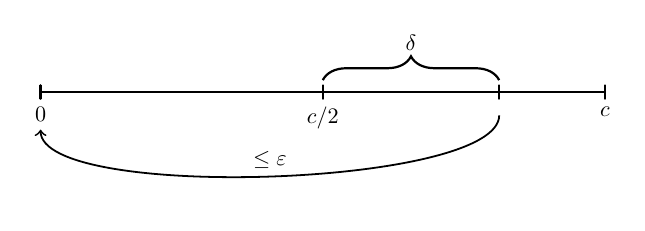
\begin{tikzpicture}[x=1.12cm, scale=0.8, every node/.append style={transform shape}]
    \draw[line width=0.2ex, line cap=round] (0,0) -- (8,0); %edit here for the axis
    \foreach \x in {0,4,6.5,8} % edit here for the vertical lines
    \draw[line width=0.2ex, line cap=round, shift={(\x,0)},color=black] (0pt,3pt) -- (0pt,-3pt);
    \foreach \x/\y/\z in {%
        0/$0$/a,
        4/${c/2}$/b,
        6.5/$$/c,
        8/$c$/d}
    \draw[line width=0.2ex, shift={(\x,0)},color=black] (0pt,0pt) -- (0pt,-3pt) node[below] (\z) {\y};

    \begin{scope}[line width=0.15ex]
        \path[->] (c) edge[out=-90, in=-90, looseness=0.4] node[above] {$\le \varepsilon$} (a);
    \end{scope}
    \draw [thick,decoration={brace,raise=1ex, amplitude=2ex},decorate] (4, 0) -- (6.5, 0) node[midway,above,yshift=3.5ex] {$\delta$};
\end{tikzpicture}


\caption{Représentation de l'état d'irréversibilité qui existe quand -- même en la présence de $f$ nœuds byzantins --
  le nombre de nœuds légitimes bleus dépasse le nombre de nœuds légitimes rouges de plus de $2\delta$.
}
\label{fig:states_feasible_solutions}
\end{center}
\end{figure}

%O \paragraph{Snowflake}
%O For Snowflake, we assume that some fraction of nodes are adversarial. In Slush, once the network gains significant majority support for one proposal (e.g., the color blue), it becomes unlikely for a minority proposal (e.g., the color red) to ever become decided in the future (irreversibility). Furthermore, in Slush nodes simply have to execute the protocol for a deterministic number of rounds, $m$, which is known ahead of protocol execution. When introducing adversarial nodes with arbitrary strategies, however, nodes cannot simply execute the protocol for a deterministic number of rounds, since the adversary may nondeterministically affect the value of $m$. Instead, correct nodes must implement a mechanism to explicitly detect that irreversibility has been reached. To that end, in Snowflake, every correct node implements a decision function, $\mathcal{D}(u, \mathcal{S}_t, blue) \rightarrow \{0, 1\}$, which is a random variable that outputs $1$ if node $u$ detects that the network has reached an irreversibility state at time $t$ for blue. The decision mechanism is probabilistic, meaning that it can fail, although it is designed to do so with negligible probability. We now sketch the proof of Snowflake.
%O
%O \noindent \emph{Proof Sketch}. We define safety failure to be the event wherein any two correct nodes $u$ and $v$ decide on blue and red, i.e. $\mathcal{D}(u, \mathcal{S}_t, blue) \rightarrow 1$ and $\mathcal{D}(v, \mathcal{S}_{t'}, red) \rightarrow 1$, for any two times $t$ and $t'$. We again model the system as a continuous time random process. The state space is defined the same way as in Slush. However, we note some critical subtleties. First, even if all correct nodes accept a color, the Byzantine nodes may revert. Second, we also have to consider the decision mechanism $\mathcal{D}(*)$. To analyze, we obviate the need to keep track of all network configurations under all adversarial strategies and assume that a node $u$ first decides on blue. Then, conditioned on the state of the network upon $u$ deciding, we calculate the probability that another node $v$ decides red, which is a function of both the probability that the network reverts towards a minority blue state and that $v$ decides at that state.
%O We show that under appropriate choices of $k$, $\alpha$, and $\beta$, we can construct highly secure instances of Snowflake (i.e. safety failure with probability $\leq \varepsilon$) when the network reaches some bias of $\delta$, as shown in Figure~\ref{fig:states_feasible_solutions}. A concrete example is provided in Figure~\ref{fig:fandepsilon}.
%O
%O \begin{figure}[h]
%O \begin{center}
%O \usetikzlibrary{decorations.pathreplacing}
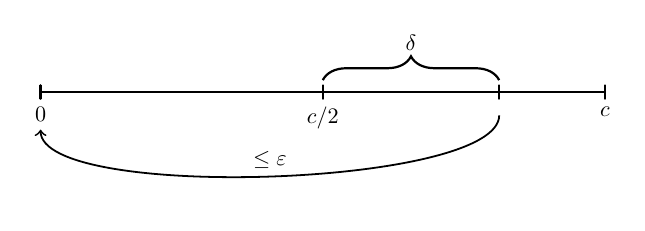
\begin{tikzpicture}[x=1.12cm, scale=0.8, every node/.append style={transform shape}]
    \draw[line width=0.2ex, line cap=round] (0,0) -- (8,0); %edit here for the axis
    \foreach \x in {0,4,6.5,8} % edit here for the vertical lines
    \draw[line width=0.2ex, line cap=round, shift={(\x,0)},color=black] (0pt,3pt) -- (0pt,-3pt);
    \foreach \x/\y/\z in {%
        0/$0$/a,
        4/${c/2}$/b,
        6.5/$$/c,
        8/$c$/d}
    \draw[line width=0.2ex, shift={(\x,0)},color=black] (0pt,0pt) -- (0pt,-3pt) node[below] (\z) {\y};

    \begin{scope}[line width=0.15ex]
        \path[->] (c) edge[out=-90, in=-90, looseness=0.4] node[above] {$\le \varepsilon$} (a);
    \end{scope}
    \draw [thick,decoration={brace,raise=1ex, amplitude=2ex},decorate] (4, 0) -- (6.5, 0) node[midway,above,yshift=3.5ex] {$\delta$};
\end{tikzpicture}


%O \caption{Representation of the irreversibility state, which exists when -- even under $f$ Byzantine nodes -- the number of blue correct nodes exceeds that of red correct nodes by more than $2\delta$.
%O }
%O \label{fig:states_feasible_solutions}
%O \end{center}
%O \end{figure}

% An important insight is that there exists an irreversible state, or \textit{point of no return}, after which the system will converge to an absorbing state whp. Furthermore a correct node only decides when the system is beyond the point of no return. Composing these two guarantees together, the probability of a safety violation is strictly less than $\varepsilon$, which can be configured as desired.
% Unsurprisingly, there is an inherent tension between safety and liveness, but suitable parameters can be found that are practical.
% Larger values of $k$ obtain higher levels of security for correct nodes, at the expense of slower convergence.

\paragraph{Snowball}

Snowball est une amélioration en terme de sécurité par rapport à Snowflake, où les perturbations aléatoires dans les
échantillons du réseau sont réduites par l'introduction d'une forme limitée d'historique que l'on appelle confiance.

\noindent \emph{Ebauche de preuve}. Nous appliquons des inégalités de concentration pour prouver qu'une fois le système
ayant atteint l'état d'irréversibilité, alors l'évolution de la confiance envers la couleur majoritaire adoptée va
augmenter constamment et dériver de plus en plus loin des nœuds de couleur minoritaire, jusqu'à rendre la réversibilité
de plus en plus improbable avec le temps. Si cette dérive finit par se retourner, alors l'analyse de la réversibilité
devient identique à celle de Snowflake.

%O \paragraph{Snowball}
%O Snowball is an improvement in security over Snowflake, where random perturbations in network samples are reduced by introducing a limited form of history, which we refer to as confidence.
%O % Modeling Snowball with a Markov chain is difficult because of a state space explosion problem. In particular, it is not sufficient to simply keep track of color preferences of each correct node, the analysis must also maintain information about their confidence.
%O
%O \noindent \emph{Proof Sketch}. We apply martingale concentration inequalities to prove that once the system has reached the irreversibility state, then the growth of the confidence of the majority decided color will perpetually grow and drift further away from those of the minority color, effectively rendering reversibility less likely over time. If the drifts ever revert, then reversibility analysis becomes identical to that of Snowflake.

\subsection{Vitalité}

Nous prenons pour hypothèse la présence antagoniste observée $0 \leq f' \leq n(k - \alpha - \psi)/k \leq f$, où $\psi$
représente la zone tampon.
Plus $\psi$ est grand, plus la capacité du mécanisme de décision à tendre vers une valeur est rapide. Bien sûr, si $\psi$
tend vers zéro ou devient négatif, alors nous dépassons la limite supérieure de tolérance antagoniste pour le système
paramétré, et en conséquence l'attaquant peut, avec une haute probabilité, bloquer la convergence en choisissant simplement
de ne pas répondre, ceci même si les garanties de sûreté de fonctionnement s'appliquent toujours.

En partant de $\psi$ strictement positif, la convergence est strictement finie pour toutes les configurations où une
proposition a un support d'au moins $\alpha$. De plus, non seulement la convergence est finie avec une probabilité de
un, mais nous avons aussi une probabilité strictement positive de convergence jusqu'à un instant borné $t_{max}$, comme
décrit dans la proposition~\ref{lemma:finitetermination}, qui découle du théorème~\ref{theorem:mean-convergence-time}.
Cela formalise la propriété de vitalité P2.

\noindent \emph{Ébauche de preuve}. En utilisant la construction du système pour prouver l'irréversibilité, nous
caractérisons la distribution de la moyenne du temps passé (les périodes de séjour) dans chaque état avant que le
système ne termine son exécution en adoptant l'un des états. Ce temps de convergence est l'union de ces périodes.

Pour les transactions non conflictuelles, l'attaquant étant incapable de générer un conflit, le temps de décision
est simplement le temps de mélange $\Oh{\log{n}}$. La vitalité guarantit qu'une configuration de réseau
entièrement bivalent atteint un temps de convergence optimal de $\Oh{\log{n}}$ tours si le nombre d'attaquants est au
plus $\Oh{\sqrt{n}}$, pour $\alpha = \floor{k/2} + 1$. Nous donnons plus de détails en
lemme~\ref{lemma:centrallimit}.
Quand le nombre de nœuds antagonistes dépasse $\Oh{\sqrt{n}}$, le nombre le moins favorable de tours grandit de manière
polynomiale, et quand $f$ tend vers $n/2$, ce nombre de tours tend vers des taux de convergence exponentiels.

\noindent \emph{Ebauche de preuve}. Nous modifions le théorème~\ref{theorem:mean-convergence-time} en y incluant le
nombre de nœuds antagonistes, ce qui annule tout déséquilibre dans le réseau en le gardant entièrement bivalent.

%O \subsection{Liveness}
%O
%O We assume that the observed adversarial presence $0 \leq f' \leq n(k - \alpha - \psi)/k \leq f$, where we refer to $\psi$ as the buffer zone.
%O The bigger $\psi$, the quicker the ability of the decision mechanism to finalize a value.
%O If, of course, $\psi$ approaches zero or becomes negative, then we violate the upper bound of adversarial tolerance for the parameterized system, and thus the adversary can, with high probability, stall termination by simply choosing to not respond, although the safety guarantees may still hold.
%O
%O Assuming that $\psi$ is strictly positive, termination is strictly finite under all network configurations where a proposal has at least $\alpha$ support. Furthermore, not only is termination finite with probability one, we also have a strictly positive probability of termination within any bounded amount of time $t_{max}$, as discussed in Lemma~\ref{lemma:finitetermination}, which follows from Theorem~\ref{theorem:mean-convergence-time}. This captures liveness property P2.
%O
%O \noindent\emph{Proof Sketch.} Using the construction of the system to prove irreversibility, we characterize the distribution of the average time spent (sojourn times) at each state before the system terminates execution by absorption at either absorbing state. The termination time is then a union of these times.
%O
%O For non-conflicting transactions, since the adversary is unable to forge a conflict, the time to decision is simply the mixing time , which is $\Oh{\log{n}}$.
%O Liveness guarantees under a fully bivalent network configuration reduce to an optimal convergence time of $\Oh{\log{n}}$ rounds if the adversary is at most $\Oh{\sqrt{n}}$, for $\alpha = \floor{k/2} + 1$. We leave additional detains to Lemma~\ref{lemma:centrallimit}.
%O % This result is independently supported by Ben-Or~\cite{ben1983another} and Doerr et al~\cite{doerr2011stabilizing}.
%O When the adversary surpasses $\Oh{\sqrt{n}}$ nodes, the worst-case number of rounds increases polynomially, and as $f$ approaches $n/2$ it approaches exponential convergence rates.
%O
%O \noindent\emph{Proof Sketch.} We modify Theorem~\ref{theorem:mean-convergence-time} to include the adversary, which reverts any imbalances in the network by keeping network fully bivalent.

\paragraph{Consensus multi-valeurs}

Notre protocole de consensus binaire pourrait supporter des consensus multi-valeurs en exécutant des instances binaires
logarithmiques, une pour chaque bit de la valeur proposée. Cependant, une telle réduction théorique n'est pas
forcément efficace en pratique. À la place, nous pourrions directement incorporer des valeurs multiples comme des
couleurs multiples dans le protocole en permettant toujours la généralisation de l'analyse de sûreté de fonctionnement.

Pour ce qui est de la vitalité, nous ébauchons en annexe~\ref{sec:sync-heuristic} un mécanisme d'initialisation sans
dirigean, qui nécessite $\Oh{\log{n}}$ tours attendus dans l'hypothèse que le réseau est synchronisé. Bien que
la conception de ce mécanisme soit intéressante, il est à noter qu'un tel mécanisme n'est pas nécessaire pour un système
de paiement décentralisé, comme nous le démontrons en section~\ref{sec:implementation}.
Finalement, nous développons le roulement, dans le sens de renouvellement des nouds, et les divergences de vues en annexe~\ref{sec:full-analysis-churn}.

%0 \paragraph{Multi-Value Consensus}
%0 Our binary consensus protocol could support multi-value consensus by running logarithmic binary instances, one for each bit of the proposed value. However, such theoretical reduction might not be efficient in practice. Instead, we could directly incorporate multi-values as multi-colors in the protocol, where safety analysis could still be generalized.
%0
%0 For liveness, we sketch a leaderless initialization mechanism, which in expectation uses $\Oh{\log{n}}$ rounds under the assumption that the network is synchronized in the Appendix~\ref{sec:sync-heuristic}.
%0 While the design of initialization mechanisms is interesting, note that it is not necessary for a decentralized payment system, as we show in Section~\ref{sec:implementation}.
%0 %We leave additional research into the initialization mechanisms to future work.
%0 %However, we finally note that when building a decentralized payment system, an initialization mechanism is not necessary, as we show in the implementation of Avalanche in Section~\ref{sec:implementation}.
%0 Finally, in the Appendix~\ref{sec:full-analysis-churn}, we discuss churn and view discrepancies.

% \subsection{Additional Insights}
% Two interesting insights arise from the way our protocols are designed and used.
% First, the protocols discussed in this work lead to both safety and liveness guarantees whose underlying function is smooth, rather than a step function.
% In many other consensus protocols, safety is guaranteed with up to a fixed threshold number (e.g.~1/3) of adversarial nodes, beyond which no guarantees are provided. In our protocols, the guarantees degrade gracefully with an adversarial percentage beyond the pre-established bound. For example, optimal system parameters can be chosen to tolerate precisely 1/5 adversarial presence with failure probability $\varepsilon$. However, if the system faces an adversarial presence greater than 1/5, then the probability of failure degrades to slightly above $\varepsilon$, rather than immediately to $1$.
% Second, these protocols externalize the safety and liveness tradeoffs.
% The system designer may choose to guarantee safety even under catastrophic events, such as an adversarial presence beyond $1/2$, at the expense of liveness.
% This presents a powerful knob not available in classical or Nakamoto-based consensus protocols.

% \begin{compactitem}
% \item\textbf{Eventually good ancestry.} Virtuous transactions can be retried by picking new parents, selected from a set that is more likely to be preferred.
% Ultimately, one can always attach a transaction to decided parents to completely mitigate this risk.
% \Jon{So why don't we always do this? Later the paper clarifies that moving up the chain reduces the efficiency
%     and increases latency for the proposed transaction. I got pretty lost in the last two paragraphs of section 4}
% A simple technique for parent selection is to select new parents for a virtuous transaction at successively lower heights in the DAG, proceeding towards the genesis vertex.
% This procedure is guaranteed to terminate with uncontested, decided parents, ensuring that the transaction cannot suffer liveness failure due to rogue transactions.

% \item\textbf{Sufficient chits.} A secondary mechanism is necessary to ensure that virtuous transactions with decided ancestry will receive sufficient chits.
% To ensure this, correct nodes examine the DAG for virtuous non-nop transactions that lack sufficient progeny and emit nop transactions to help increase their confidence.
% A nop transaction has just one parent and no application side-effects, and can be issued by any node. They cannot be abused by Byzantine nodes because, even though nops trigger new queries, they do not automatically grant chits.

% With these two mechanisms in place, it is easy to see that, at worst, Avalanche will degenerate into separate instances of Snowball, and thus provide the same liveness guarantee for virtuous transactions.
% \end{compactitem}

%XXX discuss how no-ops can be implemented

% \subsection{Communication Complexity}\tronly{}{\vspace{-0.5em}}
% Since liveness is not guaranteed for rogue transactions, we focus our message complexity analysis solely for the case of virtuous transactions.
% For the case of virtuous transactions, Snowflake and Snowball are both guaranteed to terminate after $O(kn\log n)$ messages.
% This follows from the well-known results related to epidemic algorithms\cite{demers1987epidemic}, and is confirmed by Table~\ref{table:growth_worst_case} in Appendix~\ref{sec:full-analysis}.

\section{Système de paiement pair à pair}
\label{sec:implementation}

%\label{sec:evaluation}

%O Using Snowball consensus, we have implemented a bare-bones payment system, Avalanche, which supports Bitcoin transactions. In this section, we describe the design and sketch how the implementation can support the value transfer primitive at the center of cryptocurrencies.
Grâce au consensus Snowball, nous avons implémenté un système de paiement élémentaire, Avalanche, qui supporte les transactions Bitcoin. Dans cette section, nous en décrivons la conception et schématisons la manière dont l'implémentation peut supporter la primitive de transfert de valeur au cœur des cryptomonnaies.
%O Deploying a full cryptocurrency involves bootstrapping, minting, staking, unstaking,
%O and inflation control. While we have solutions for these issues, their full
%O discussion is beyond the scope of this paper, whose focus is centered on the
%O novel Snow consensus protocol family.
Le déploiement complet d'une cryptomonnaie implique l'initialisation, l'émission, le dépôt, le retrait et le contrôle de l'inflation. Nous disposons de solutions à ces problèmes mais leur description détaillée sort du cadre de cet article, dont l'objet est la nouvelle famille de consensus Snow.
%In this section,
%we focus on how Avalanche can support the value transfer primitive at the center of cryptocurrencies.
%\paragraph{XXX: the original implementation paragraph in Model}

%The Snow family is presented in the form of single-decree, binary consensus for its own theoretical value and simplicity.
%On the other hand, we show later in Section~\ref{sec:implementation} our practical payment system, Avalanche, utilizes multiple Snowball instances to support standard Bitcoin-like transactions. %, by humbly cheating in two ways.
%First, instead of a single replicated state machine (RSM) model, where the system determines a sequence of totally-ordered transactions $T_0, T_1, T_2, \ldots$ issued by any client, we adopt a \emph{parallel consensus model}, where each client interacts independently with its own RSMs and optionally transfers ownership of its RSM to another client. The system establishes only a partial order between dependent transactions.
%Second,
%O In a cryptocurrency setting, cryptographic signatures enforce that only a key owner is able to create a transaction that spends a particular coin. Since correct clients follow the protocol as prescribed and never double spend coins, in Avalanche, they are guaranteed both safety and liveness for their \emph{virtuous} transactions. In contrast, liveness is not guaranteed for \emph{rogue} transactions, submitted by Byzantine clients, which conflict with one another. Such decisions may stall in the network, but have no safety impact on virtuous transactions.
Dans une configuration de cryptomonnaie, les signatures cryptographiques imposent que seul le possesseur de la clef soit capable de créer une transaction dépensant un dépôt donné. Comme les clients corrects suivent le protocole tel qu'il est prescrit et ne peuvent pratiquer la double dépense, ils ont la garantie tant de la sûreté de fonctionnement que de la vitalité pour leurs transactions \emph{vertueuses}. Par contraste, la vitalité n'est pas garantie pour les transactions \emph{malveillantes} soumises par des clients byzantins, lesquelles entrent mutuellement en conflit. Ces décisions peuvent arrêter le réseau mais n'ont pas d'impact sur les transactions vertueuses.
%O We show that this is a sensible tradeoff, and that the resulting system is sufficient for building complex payment systems.
Nous montrons que ce compromis est raisnnable et que le système qui en résulte suffit à bâtir des systèmes de paiement complexes.

\subsection{Avalanche\,: ajout d'un DAG}%\tronly{}{\vspace{-0.5em}}

%O Avalanche consists of multiple single-decree Snowball instances instantiated as a multi-decree protocol that
%O maintains a dynamic, append-only directed acyclic graph (DAG) of all known transactions.
Avalanche consiste en plusieurs instance Snowball à décret unique instanciées en tant que protocole multi-décrets qui maintient un graphe orienté acyclique (\emph{Directed Acyclic Graph},  DAG) dynamique en ajout seul de toutes les transactions connues.
%O The DAG has a single sink that is the \emph{genesis vertex}.
Le DAG possède un nœud terminal (\emph{sink}) unique qui est le \emph{genesis vertex}, le sommet genèse.
%O Maintaining a DAG provides two significant benefits.
L'emploi d'un DAG procure deux avantages\,:
%O First, it improves efficiency, because a single vote on a DAG vertex implicitly votes for all tran
%O sactions on the path to the genesis vertex.
D'abord, il est plus efficient car un vote sur un sommet vote implicitement pour toutes les transactions se trouvant sur le chemin du sommet genèse.
%O Second, it also improves security, because the DAG intertwines the fate of transactions, similar to the Bitcoin blockchain.
Ensuite, il améliore également la sécurité parce que le DAG lie fortement le sort des transactions, similaire en cela à la blockchain de Bitcoin.
%O This renders past decisions difficult to undo without the approval of correct nodes.
Cela rend les décisions passées difficiles à défaire sans l'approbation des nœuds corrects.


% Avalanche's DAG embodies all the transactions that have been proposed to the system, where each transaction is represented as a vertex.
% The DAG is rooted at a protocol-defined, well-known \emph{genesis} vertex.
%O When a client creates a transaction, it names one or more \emph{parents}, which are included inseparably in the transaction and form the edges of the DAG\@.
Quand un client crée une transaction, il nomme un ou plusieurs \emph{parents}, et ceux-ci sont inclus de façon inséparable dans la transaction et forment les bords du DAG\@.
%O The parent-child relationships encoded in the DAG may, but do not need to, correspond to application-specific dependencies; for instance, a child transaction need not spend or have any relationship with the funds received in the parent transaction.
Les relations parent-enfant codées dans le DAG peuvent, sans obligation, correspondre à des dépendances spécifiques aux applications\,; par exemple, la transaction d'un enfant ne dépense pas nécessairement, ni n'a forcément de relation avec les fonds reçus lors de la transaction parent.
% These additional relationships entangle the fate of previous decisions made by the system.
%O We use the term \emph{ancestor set} to refer to all transactions reachable via parent edges back in history, and \emph{progeny} to refer to all children transactions and their offspring.
Nous utilisons le terme \emph{ensemble ancêtre} pour nous référer à toutes les transactions accessibles par les arêtes parent historisées, et \emph{progéniture} pour nous référer à toutes les transactions enfant et leur descendance.

%O The central challenge in the maintenance of the DAG is to choose among \emph{conflicting transactions}.
Le principal défi de la maintenance du DAG est de choisir parmi des \emph{transactions conflictuelles}.
%O The notion of conflict is application-defined and transitive, forming an equivalence relation.
La notion de conflit est définie par l'application et est transitive, formant une relation d'équivalence.
%O In our cryptocurrency application, transactions that spend the same funds (\emph{double-spends}) conflict, and form a \emph{conflict set}
%(Figure~\tronly{\ref{fig:dag-conflict-set}}{\ref{fig:dag-cd}})
%O (shaded regions in Figure~\ref{fig:dag-cd}), out of which only a single one can be accepted.
Dans notre application de cryptomonnaie, les transactions qui dépensent les mêmes fonds (\emph{double-dépense}) entrent en conflit et forment un \emph{ensemble de conflits}
(régions ombrées en figure~\ref{fig:dag-cd}), duquel une seule peut être acceptée.
%O Note that the conflict set of a virtuous transaction is always a singleton.
On note que l'ensemble de conflits d'une transaction vertueuse est toujours un singleton.
%Note that the graph structure of transactions that spend depend on each other, also known as the UTXO graph, is completely independent of the DAG that Avalanche maintains. As a result, any two vertices may be in conflict. Figure~\ref{fig:dag-conflicting-set} shows an example.
 
%\tronly{
%\begin{figure}\begin{center}
%    \definecolor{lightgray}{HTML}{dddddd}
\definecolor{medgray}{HTML}{cccccc}
\definecolor{medgray2}{HTML}{bbbbbb}
\definecolor{darkgray}{HTML}{aaaaaa}
\definecolor{lightgp}{HTML}{ddddee}
\begin{tikzpicture}[x=1.12cm]
    \begin{scope}[all/.style={draw,fill=white,minimum height=0.5cm, minimum width=0.5cm},line width=0.08ex]
        \node[fill=lightgp, circle,minimum width=1cm] (pt1) at (0, 0) {};
        \node[fill=lightgp, circle,minimum width=1cm] (pt4) at (-1.5, -2) {};
        \node[fill=lightgp, circle,minimum width=1cm] (pt5) at (-0.5, -2) {};
        \node[fill=lightgp, circle,minimum width=1cm] (pt6) at (-2, -3) {};
        \fill[color=lightgp] plot[smooth cycle] coordinates { (1.2, -1) (0.9, -1.4) (-0.9, -1.4) (-1.2, -1) (-0.9, -0.6) (0.9, -0.6)} node (pt2) {};
        \fill[color=lightgp] plot[smooth cycle] coordinates {(2.1, -1.75) (2, -2.4) (0.6, -3.4) (0, -3.5) (-0.3, -3.3)(-0.3, -2.8) (0.1, -2.4) (1.2, -1.65) (1.7, -1.5) } node (pt3) {};
        \node[all, draw] (b0) at (0, 0) {$T_1$};
        \node[all, draw] (b1) at (-0.8, -1) {$T_2$};
        \node[all, draw] (b2) at (0.8, -1) {$T_3$};
        \node[all, draw] (b3) at (-1.5, -2) {$T_4$};
        \node[all, draw] (b4) at (-0.5, -2) {$T_5$};
        \node[all, draw] (b5) at (0.9, -2.5) {$T_6$};
        \node[all, draw] (b6) at (1.7, -2) {$T_7$};
        \node[all, draw] (b7) at (-2, -3) {$T_8$};
        \node[all, draw] (b8) at (0.2, -3) {$T_9$};
        \begin{scope}[line width=0.2ex]
        \path[->] (b1) edge[out=90, in=-110] node[sloped,above] {} (b0) ;
        \path[->] (b2) edge[out=100, in=-70] node[sloped,above] {} (b0) ;
        \path[->] (b3) edge[out=90, in=-110] node[sloped,above] {} (b1) ;
        \path[->] (b4) edge[out=90, in=-70] node[sloped,above] {} (b1) ;
        \path[->] (b5) edge[out=100, in=-110] node[sloped,above] {} (b2) ;
        \path[->] (b6) edge[out=120, in=-70] node[sloped,above] {} (b2) ;
        \path[->] (b7) edge[out=90, in=-90] node[sloped,above] {} (b3) ;
        \path[->] (b7) edge[out=0, in=-110] node[sloped,above] {} (b4) ;
        \path[->] (b8) edge[out=90, in=-70] node[sloped,above] {} (b4) ;
        \end{scope}
        \node[] (p1) at (3, 0.5) {\footnotesize$\mathcal{P}_{T_1}$};
        \node[] (p2) at (3, 0) {\footnotesize$\mathcal{P}_{T_2} = \mathcal{P}_{T_3}$};
        \node[] (p3) at (3, -0.5) {\footnotesize$\mathcal{P}_{T_9} = \mathcal{P}_{T_6} = \mathcal{P}_{T_7}$};
        \begin{scope}[color=darkgray,dashed,line width=0.2ex]
        \path[->] (p1) edge[out=180, in=0] node[sloped,above] {} (pt1) ;
        \path[->] (p2) edge[out=180, in=60] node[sloped,above] {} (pt2) ;
        \path[->] (p3) edge[out=-90, in=30] node[sloped,above] {} (pt3) ;
        \end{scope}
    \end{scope}
\end{tikzpicture}

%    \captionof{figure}{DAG vertices partitioned by conflict sets. At most one vertex in each shaded region will be accepted.}\label{fig:dag-conflict-set}
%\end{center}
%\end{figure}
%}{}

%O Avalanche instantiates a Snowball instance for each conflict set.
Avalanche instancie une instance de Snowball pour chaque ensemble de conflit.
%O Whereas Snowball uses repeated queries and multiple counters to capture the amount of confidence built in conflicting transactions (colors),
%O Avalanche takes advantage of the DAG structure and uses a transaction's progeny.
Alors que Snowball utilise des requêtes répétées et plusieurs compteurs pour obtenir le degré de confiance associé aux transactions conflictuelles (couleurs),
Avalanche profite de la structure du DAG et utilise la progéniture d'une transaction.
%O Specifically, when a transaction $T$ is queried, all transactions reachable from $T$ by following the DAG edges are implicitly part of the query.
En particulier, quand on interroge une transaction $T$, toutes les transactions accessible depuis $T$ en suivant les arêtes du DAG font implicitement partie de la requête.
%O A node will only respond positively to the query if $T$ and its entire ancestry are currently the preferred option in their respective conflict sets.
Un nœud ne répond positivement à la requête que si $T$ et toute son ascendance représente actuellement l'option préférentielle dans leurs ensembles de conflits respectifs.
%O If more than a threshold of responders vote positively, the transaction is said to collect a \emph{chit}.
Si un nombre de nœuds répondant positivement est supérieur au seuil, on dit que la transaction récolte un \emph{chit} (un bon).
%O Nodes then compute their \emph{confidence} as the total number of chits in the progeny of that transaction.
Les nœuds calculent ensuite leur \emph{confiance} en comptant le nombre de chits dans la progéniture de cette transaction.
%O They query a transaction just once and rely on new vertices and possible chits, added to the progeny, to build up their confidence.
Ils n'envoient qu'une seule requête et se basent sur les nouveaux sommets les chits possibles, ajoutés à la progéniture, pour fonder leur confiance.
%O Ties are broken by an initial preference for first-seen transactions.
Les liens sont brisés par une préférence initiale pour les transactions vues en premier.
%O Note that chits are decoupled from the DAG structure, making the protocol immune to attacks where
%O the attacker generates large, padded subgraphs.
On note que les chits sont découplés de la structure du DAG, rendant le protocole immune aux attaques où un attaquant génère de grands sous-graphes remplis de fausses valeurs.

%O \subsection{Avalanche: Specification}%\tronly{}{\vspace{-0.5em}}
\subsection{Avalanche\,: Spécification}%\tronly{}{\vspace{-0.5em}}
\label{subsection:specification}

\newcommand{\codeedges}{\mathit{edges}}
\newcommand{\codedata}{\mathit{data}}
\begin{figure}
\begin{center}
\small
\begin{algorithmic}[1]
    \Procedure{init}{}
%O        \State $\mathcal{T} \assign \emptyset$ \hspace{1ex}\textrm{// the set of known transactions}
%O        \State $\mathcal{Q} \assign \emptyset$ \hspace{1ex}\textrm{// the set of queried transactions}
        \State $\mathcal{T} \assign \emptyset$ \hspace{1ex}\textrm{// l'ensemble des transactions connues}
        \State $\mathcal{Q} \assign \emptyset$ \hspace{1ex}\textrm{// l'ensemble des transactions interrogées}
    \EndProcedure
    \Procedure{onGenerateTx}{$\codedata$}
        \State $\codeedges \assign \{T' \gets T: T' \in \Call{parentSelection}{\mathcal{T}}\}$
        \State $T \assign \Call{Tx}{\codedata, \codeedges}$
        \State \Call{onReceiveTx}{$T$}
    \EndProcedure
    \Procedure{onReceiveTx}{$T$}
        \If{$T \notin \mathcal{T}$}
            \If{$\mathcal{P}_T = \emptyset$}
                \State $\mathcal{P}_T \assign \{T\}$, $\mathcal{P}_T\mathit{.pref} \assign T$
                \State $\mathcal{P}_T\mathit{.last} \assign T, \mathcal{P}_T\mathit{.cnt} \assign 0$
            \Else$\ \mathcal{P}_T \assign \mathcal{P}_T \cup \{T\}$
            \EndIf
            \State $\mathcal{T} \assign \mathcal{T} \cup \{T\}$, $c_T \assign 0$.
        \EndIf
    \EndProcedure
%O    \captionof{figure}{Avalanche: transaction generation.}\label{fig:gossipchain-ongen}
    \captionof{figure}{Avalanche\,: génération des transactions.}\label{fig:gossipchain-ongen}
\end{algorithmic}
\end{center}
\end{figure}

\begin{figure}
\begin{center}
\small
\begin{algorithmic}[1]
    \Procedure{avalancheLoop}{}
        \While {\codetrue}
%O            \State\textrm{find  $T$ that satisfies }%\vspace*{-.6\baselineskip}
            \State\textrm{trouver  $T$ satisfaisant }%\vspace*{-.6\baselineskip}
            $T \in \mathcal{T} \land T \notin \mathcal{Q}$
            %\begin{align*}\hspace{2ex}
            %    T \in \mathcal{T} &\land T \notin \mathcal{Q} \\
            %            &\land (\forall T', T' \gets T: T' \in \mathcal{Q})
            %\end{align*}
            \State $\mathcal{K} \assign \Call{sample}{\mathcal{N}\backslash u, k}$
            \State $P \assign \sum_{v \in \mathcal{K}}\Call{query}{v, T}$
            \If{$P \ge \alpha$}
                \State $c_T \assign 1$
%O            \State\textrm{// update the preference for ancestors}
            \State\textrm{// mettre à jour les préférences pour les ancêtres}
            \For{$T' \in \mathcal{T} : T' \stackrel{*}{\gets} T$}
                \If{$d(T') > d(\mathcal{P}_{T'}\mathit{.pref})$}
                    \State $\mathcal{P}_{T'}\mathit{.pref} \assign T'$
                \EndIf
                \If{$T'\neq \mathcal{P}_{T'}\mathit{.last}$}
                    \State $\mathcal{P}_{T'}\mathit{.last} \assign T'$, $\mathcal{P}_{T'}\mathit{.cnt} \assign 1$
                \Else
                    \State \texttt{++}$\mathcal{P}_{T'}\mathit{.cnt}$
                \EndIf
            \EndFor
            \Else
            \For{$T' \in \mathcal{T} : T' \stackrel{*}{\gets} T$}
                    \State$\mathcal{P}_{T'}\mathit{.cnt} \assign 0$
            \EndFor
            \EndIf
%O            \State\textrm{// otherwise, }$c_T$\textrm{ remains 0 forever}
            \State\textrm{// sinon, }$c_T$\textrm{ reste éternellement à 0}
%O            \State $\mathcal{Q} \assign \mathcal{Q} \cup \{T\}$ \hspace {1ex} \textrm{// mark T as queried}
            \State $\mathcal{Q} \assign \mathcal{Q} \cup \{T\}$ \hspace {1ex} \textrm{// marquer T comme interrogé}
        \EndWhile
    \EndProcedure
%O    \captionof{figure}{Avalanche: the main loop.}\label{fig:gossipchain-main}
    \captionof{figure}{Avalanche\,: boucle principale.}\label{fig:gossipchain-main}
\end{algorithmic}
\end{center}
\end{figure}

% TODO IMPORTANT The isPreferred must imply that T is queried, but current writing can be not queried. Also, do you do max over only queried transactions?
\begin{figure}[t]
\begin{center}
\small
\begin{algorithmic}[1]
    \Function{isPreferred}{$T$}
        %\State \Return $d(T) = \max_{T' \in \mathcal{P}_T} d(T')$
        \State \Return $T = \mathcal{P}_T\mathit{.pref}$
    \EndFunction
    \Function{isStronglyPreferred}{$T$}
        \State \Return $\forall T'\in\mathcal{T}, T' \stackrel{*}{\gets} T: \Call{isPreferred}{T'}$
    \EndFunction
    \Function{isAccepted}{$T$}
        \State\Return
            \vspace*{-.5\baselineskip}
        \begin{align*}
            (&(\forall T' \in \mathcal{T}, T' \gets T: \Call{isAccepted}{T'}) \\
                &\land |\mathcal{P}_T| = 1 \land \mathcal{P}_T\mathit{.cnt} \ge \beta_1) \texttt{\hspace{.1in}// engagement préalable sûr} \\
            %& \left(\frac{d(T)}{d'} > \gamma \land d' \ge \beta_2\right)
            \lor &(%\mathcal{P}_T\textrm{.pref} = \mathcal{P}_T\textrm{.last} \land
            \mathcal{P}_T\mathit{.cnt} \ge \beta_2)\texttt{\hspace{.1in}// compteur consécutif}
        \end{align*}
    \EndFunction
    \Procedure{onQuery}{$j, T$}
        \State \Call{onReceiveTx}{$T$}
        \State \Call{respond}{$j, \textsc{isStronglyPreferred}(T)$}
    \EndProcedure
    \captionof{figure}{Avalanche\,: primitives de vote et de décision.}\label{fig:gossipchain-onquery}
\end{algorithmic}
\end{center}
\end{figure}

%O Each correct node $u$
%O keeps track of all transactions it has learned about in set $\mathcal{T}_u$,
%O partitioned into mutually exclusive conflict sets $\mathcal{P}_T$, $T \in \mathcal{T}_u$.
Chaque nœud correct $u$ conserve la trace de toutes les transactions dont il a été informé dans l'ensemble $\mathcal{T}_u$, partitionné en ensembles de conflits mutuellement exclusifs $\mathcal{P}_T$, $T \in \mathcal{T}_u$.
% Transactions are determined to be conflicting based on a deterministic function known to every node.
%O Since conflicts are transitive, if $T_i$ and $T_j$ are conflicting, then they belong to the same conflict set, i.e. $\mathcal{P}_{T_i} = \mathcal{P}_{T_j}$. This relation may sound counter-intuitive: conflicting transitions have the \emph{equivalence} relation, because they are equivocations spending the \emph{same} funds.
Comme les conflits sont transitifs, si $T_i$ et $T_j$ sont en conflit, ils appartiennent au même ensemble de conflits, c'est-à-dire $\mathcal{P}_{T_i} = \mathcal{P}_{T_j}$. Cette relation peut sembler contre-intuitive\,: les transactions en conflit ont la même relation d'\emph{équivalence} car ce sont des équivoques dépensant les \emph{mêmes} fonds.
%\Jon{By $=$ surely you mean $\neq$?}

%O We write $T' \gets T$ if $T$ has a parent edge to transaction $T'$,
Nous écrivons $T' \gets T$ si $T$ a une arête commune avev la transaction $T'$.
%O The ``$\stackrel{*}{\gets}$''-relation is its reflexive transitive closure, indicating a path from $T$ to $T'$.
La relation ``$\stackrel{*}{\gets}$'' est sa fermeture réflexive transitive, indiquant un chemin de $T$ vers $T'$.
%O DAGs built by different nodes are guaranteed to be compatible, though at any one time, the two nodes may not have a complete view of all vertices in the system.
Les DAG construits par des nœuds différents offrent la garantie d'être compatibles, bien qu'à un moment donné les nœuds puissent ne pas avoir une vue complète de tous les sommets dans le système.
%O Specifically, if $T' \gets T$, then every node in the system that has $T$ will also have $T'$ and the same relation $T' \gets T$; and conversely, if $T' \cancel{\gets} T$, then no nodes will end up with $T' \gets T$.
En particulier, si $T' \gets T$, alors tout nœud dans le système qui possède $T$ aura également $T'$ et la même relation $T' \gets T$ ; inversement, si f $T' \cancel{\gets} T$, alors aucun nœud n'arrivera à $T' \gets T$.

%O Each node $u$ can compute a confidence value, $d_u(T)$, from the progeny as follows:
Chaque nœud $u$ peut calculer une valeur de confiance $d_u(T)$ de sa progéniture comme suit\,:
\[ d_u(T) = \sum_{T' \in \mathcal{T}_u, T \stackrel{*}{\gets} T'}c_{uT'}\]
%O where $c_{uT'}$ stands for the chit value of $T'$ for node $u$. Each transaction initially has a chit value of $0$ before the node gets
%O the query results. If the node collects a threshold of $\alpha$ yes-votes after the query, the value $c_{uT'}$ is set to 1, otherwise remains $0$ forever.
où $c_{uT'}$ représente la valeur de chit de $T'$ pour le nœud $u$. Chaque transaction a un valeur de chit à $0$ avant que le nœud obtienne les résultats des requêtes. Si le nœud récolte un seuil de $\alpha$ votes «\,oui\,» après la requête, la valeur $c_{uT'}$ est mise à 1, sinon elle reste éternellement à $0$.
%O Therefore, a chit value reflects the result from the one-time query of its associated transaction and becomes immutable afterwards, while $d(T)$ can increase as the DAG grows by collecting more chits in its progeny.
Donc, une valeur de chit reflète le résultat de la requête à un moment donné de ses transactions associées et devient immuable après cela, alors que $d(T)$ peut augmenter au fur et à mesure de la croissance du DAG en collectant d'autres chits dans sa progéniture.
%O Because $c_T \in \{0, 1\}$, confidence values are monotonic.
Comme $c_T \in \{0, 1\}$, les valeurs de confiance sont monotones.
%\Jon{the notation $c_{uT}$ shows up before it's definet. I guess it's the number of chits counted for $T$ by participant $u$?}

%O In addition, node $u$ maintains its own local list of known nodes $\mathcal{N}_u \subseteq \mathcal{N}$ that comprise the system.
De plus, le nœud $u$ maintient sa propre liste locale de nœuds connus $\mathcal{N}_u \subseteq \mathcal{N}$ qui constituent le système.
%O For simplicity, we assume for now $\mathcal{N}_u = \mathcal{N}$, and elide subscript $u$ in contexts without ambiguity.
Dans un souci de simplicité, nous supposons pour l'instant que $\mathcal{N}_u = \mathcal{N}$, et nous éludons le $u$ souscrit dans les contextes sans ambiguïté.
%
% TODO talk to ted and ask how to rephrase this. "the data structure" is unclear, and so is immutability
% This is because a transaction is immutable in the sense that its identity is uniquely determined by both the application data and parent links it embodies.
%Here, notation ``$T' \gets T$'' means $T'$ is one of $T$'s immediate parents, and
%``$\stackrel{*}{\gets}$''-relation is the reflexive transitive closure of ``$\gets$''-relation; namely,
%if $T' \stackrel{*}{\gets} T$, there exists a path from $T$ to $T'$. Specially, ``$T \stackrel{*}{\gets} T$''.

%O Each node implements an event-driven state machine, centered around a query that serves both to solicit votes on each transaction and to notify other nodes of the existence of newly discovered transactions.
Chaque nœud implémente une machine à état orientée événements, centrée autour d'une requête qui sert à la fois à solliciter des votes pour chaque transaction et à notifier d'autres nœuds de l'existence de transactions nouvellement découvertes.
%O In particular, when node $u$ discovers a transaction $T$ through a query, it starts a one-time query process by sampling $k$ random peers and sending a message to them, after $T$ is delivered via $\textsc{onReceiveTx}$.
En particulier, quand le nœud $u$ découvre une transaction $T$ au cours d'une requête, il commence un processus de requête unique % HOULA one-time query
en échantillonnant $k$ pairs au hasard et en leur envoyant un message après que $T$ a été délivré par $\textsc{onReceiveTx}$.
% determining the set of conflicting transactions $\mathcal{P}_T$,

%O Node $u$ answers a query by checking whether each $T'$ such that $T' \stackrel{*}{\gets} T$ is currently preferred among competing transactions $\forall T'' \in \mathcal{P}_{T'}$.
Le nœud $u$ répond à une requête en vérifiant si chaque $T'$ telle que $T' \stackrel{*}{\gets} T$ est actuellement préférée par rapport aux transactions concurrentes $\forall T'' \in \mathcal{P}_{T'}$.
%O If every single ancestor $T'$ fulfills this criterion, the transaction is said to be \emph{strongly preferred}, and receives a yes-vote (1). A failure of this criterion at any $T'$ yields a no-vote (0).
Si chacun des ancêtres $T'$ répond à ce critère, la transaction est dite \emph{fortement préférée}, et reçoit un vote oui (1). Un manquement à ce critère pour toute $T'$ engendre un vote non (0).
%O When $u$ accumulates $k$ responses, it checks whether there are $\alpha$ yes-votes for $T$, and if so grants the chit (chit value $c_T \assign 1$) for $T$.
Quand $u$ accumule $k$ réponses, il vérifie s'il existe
%O The above process will yield a labeling of the DAG with a chit value and associated confidence for each transaction~$T$.
Le processus ci-dessus ramène un étiquetage du DAG avec une valeur de chit et une confiance associée pour chaque transaction~$T$.

\begin{figure}
\begin{center}
    %\tronly{\definecolor{lightgray}{HTML}{dddddd}
\definecolor{medgray}{HTML}{cccccc}
\definecolor{medgray2}{HTML}{bbbbbb}
\definecolor{darkgray}{HTML}{aaaaaa}
\definecolor{lightgp}{HTML}{ddddee}
\begin{tikzpicture}[x=1.12cm, scale=0.9, every node/.append style={transform shape}]
    \begin{scope}[all/.style={draw, minimum height=0.5cm, minimum width=0.5cm},line width=0.08ex]
        \node[fill=lightgp, circle,minimum width=1cm] (pt1) at (0, 0) {};
        \node[fill=lightgp, circle,minimum width=1cm] (pt4) at (-1.5, -2) {};
        \node[fill=lightgp, circle,minimum width=1cm] (pt5) at (-0.5, -2) {};
        \node[fill=lightgp, circle,minimum width=1cm] (pt6) at (-2, -3) {};
        \fill[color=lightgp] plot[smooth cycle] coordinates { (1.2, -1) (0.9, -1.4) (-0.9, -1.4) (-1.2, -1) (-0.9, -0.6) (0.9, -0.6)} node (pt2) {};
        \fill[color=lightgp] plot[smooth cycle] coordinates {(2.1, -1.75) (2, -2.4) (0.6, -3.4) (0, -3.5) (-0.3, -3.3)(-0.3, -2.8) (0.1, -2.4) (1.2, -1.65) (1.7, -1.5) } node (pt3) {};
        \node[all, draw,fill=darkgray] (b0) at (0, 0) {$T_1$};
        \node[all, draw,fill=darkgray] (b1) at (-0.8, -1) {$T_2$};
        \node[all, draw,fill=white] (b2) at (0.8, -1) {$T_3$};
        \node[all, draw,fill=medgray] (b3) at (-1.5, -2) {$T_4$};
        \node[all, draw,fill=medgray2] (b4) at (-0.5, -2) {$T_5$};
        \node[all, draw,fill=white] (b5) at (0.9, -2.5) {$T_6$};
        \node[all, draw,fill=white] (b6) at (1.7, -2) {$T_7$};
        \node[all, draw,fill=lightgray] (b7) at (-2, -3) {$T_8$};
        \node[all, draw,fill=lightgray] (b8) at (0.2, -3) {$T_9$};
        \begin{scope}[line width=0.2ex]
        \path[->] (b1) edge[out=90, in=-110] node[sloped,above] {} (b0) ;
        \path[->] (b2) edge[out=100, in=-70] node[sloped,above] {} (b0) ;
        \path[->] (b3) edge[out=90, in=-110] node[sloped,above] {} (b1) ;
        \path[->] (b4) edge[out=90, in=-70] node[sloped,above] {} (b1) ;
        \path[->] (b5) edge[out=100, in=-110] node[sloped,above] {} (b2) ;
        \path[->] (b6) edge[out=120, in=-70] node[sloped,above] {} (b2) ;
        \path[->] (b7) edge[out=90, in=-90] node[sloped,above] {} (b3) ;
        \path[->] (b7) edge[out=0, in=-110] node[sloped,above] {} (b4) ;
        \path[->] (b8) edge[out=90, in=-70] node[sloped,above] {} (b4) ;
        \end{scope}
        %\node[] (p1) at (3, 0.5) {\footnotesize$\mathcal{P}_{T_1}$} ;
        %\node[] (p2) at (3, 0) {\footnotesize$\mathcal{P}_{T_2} = \mathcal{P}_{T_3}$};
        %\node[] (p3) at (3, -0.5) {\footnotesize$\mathcal{P}_{T_9} = \mathcal{P}_{T_6} = \mathcal{P}_{T_7}$};
        %\begin{scope}[color=darkgray,dashed,line width=0.2ex]
        %\path[->] (p1) edge[out=180, in=0] node[sloped,above] {} (pt1) ;
        %\path[->] (p2) edge[out=180, in=60] node[sloped,above] {} (pt2) ;
        %\path[->] (p3) edge[out=-90, in=30] node[sloped,above] {} (pt3) ;
        %\end{scope}

        \node[anchor=south, yshift=0.1cm] at (b0.north) {\footnotesize$\langle \mathbf{c_{T_1}}, d(T_1) \rangle = \langle\mathbf{1}, 6\rangle$};
        \node[anchor=east,xshift=-0.1cm] at (b1.west) {\footnotesize$\langle \mathbf{1}, 5 \rangle$};
        \node[anchor=west,xshift=0.1cm] at (b2.east) {\footnotesize$\langle \mathbf{0}, 0 \rangle$};
        \node[anchor=east,xshift=-0.1cm] at (b3.west) {\footnotesize$\langle \mathbf{1}, 2 \rangle$};
        \node[anchor=west,xshift=0.1cm] at (b4.east) {\footnotesize$\langle \mathbf{1}, 3 \rangle$};
        \node[anchor=north west,xshift=0.1cm] at (b5.south east) {\footnotesize$\langle \mathbf{0}, 0 \rangle$};
        \node[anchor=north west] at (b6.south east) {\footnotesize$\langle \mathbf{0}, 0 \rangle$};
        \node[anchor=north west] at (b8.south east) {\footnotesize$\langle \mathbf{1}, 1 \rangle$};
        \node[anchor=north,yshift=-0.2cm] at (b7.south) {\footnotesize$\langle \mathbf{1}, 1 \rangle$};
        
    \end{scope}
\end{tikzpicture}
}{\definecolor{lightgray}{HTML}{dddddd}
\definecolor{medgray}{HTML}{cccccc}
\definecolor{medgray2}{HTML}{bbbbbb}
\definecolor{darkgray}{HTML}{aaaaaa}
\definecolor{lightgp}{HTML}{ddddee}
\begin{tikzpicture}[x=1.12cm, scale=0.9, every node/.append style={transform shape}]
    \begin{scope}[all/.style={draw, minimum height=0.5cm, minimum width=0.5cm},line width=0.08ex]
        \node[fill=lightgp, circle,minimum width=1cm] (pt1) at (0, 0) {};
        \node[fill=lightgp, circle,minimum width=1cm] (pt4) at (-1.5, -2) {};
        \node[fill=lightgp, circle,minimum width=1cm] (pt5) at (-0.5, -2) {};
        \node[fill=lightgp, circle,minimum width=1cm] (pt6) at (-2, -3) {};
        \fill[color=lightgp] plot[smooth cycle] coordinates { (1.2, -1) (0.9, -1.4) (-0.9, -1.4) (-1.2, -1) (-0.9, -0.6) (0.9, -0.6)} node (pt2) {};
        \fill[color=lightgp] plot[smooth cycle] coordinates {(2.1, -1.75) (2, -2.4) (0.6, -3.4) (0, -3.5) (-0.3, -3.3)(-0.3, -2.8) (0.1, -2.4) (1.2, -1.65) (1.7, -1.5) } node (pt3) {};
        \node[all, draw,fill=darkgray] (b0) at (0, 0) {$T_1$};
        \node[all, draw,fill=darkgray] (b1) at (-0.8, -1) {$T_2$};
        \node[all, draw,fill=white] (b2) at (0.8, -1) {$T_3$};
        \node[all, draw,fill=medgray] (b3) at (-1.5, -2) {$T_4$};
        \node[all, draw,fill=medgray2] (b4) at (-0.5, -2) {$T_5$};
        \node[all, draw,fill=white] (b5) at (0.9, -2.5) {$T_6$};
        \node[all, draw,fill=white] (b6) at (1.7, -2) {$T_7$};
        \node[all, draw,fill=lightgray] (b7) at (-2, -3) {$T_8$};
        \node[all, draw,fill=lightgray] (b8) at (0.2, -3) {$T_9$};
        \begin{scope}[line width=0.2ex]
        \path[->] (b1) edge[out=90, in=-110] node[sloped,above] {} (b0) ;
        \path[->] (b2) edge[out=100, in=-70] node[sloped,above] {} (b0) ;
        \path[->] (b3) edge[out=90, in=-110] node[sloped,above] {} (b1) ;
        \path[->] (b4) edge[out=90, in=-70] node[sloped,above] {} (b1) ;
        \path[->] (b5) edge[out=100, in=-110] node[sloped,above] {} (b2) ;
        \path[->] (b6) edge[out=120, in=-70] node[sloped,above] {} (b2) ;
        \path[->] (b7) edge[out=90, in=-90] node[sloped,above] {} (b3) ;
        \path[->] (b7) edge[out=0, in=-110] node[sloped,above] {} (b4) ;
        \path[->] (b8) edge[out=90, in=-70] node[sloped,above] {} (b4) ;
        \end{scope}
        \node[] (p1) at (3, 0.5) {\footnotesize$\mathcal{P}_{T_1}$} ;
        \node[] (p2) at (3, 0) {\footnotesize$\mathcal{P}_{T_2} = \mathcal{P}_{T_3}$};
        \node[] (p3) at (3, -0.5) {\footnotesize$\mathcal{P}_{T_9} = \mathcal{P}_{T_6} = \mathcal{P}_{T_7}$};
        \begin{scope}[color=darkgray,dashed,line width=0.2ex]
        \path[->] (p1) edge[out=180, in=0] node[sloped,above] {} (pt1) ;
        \path[->] (p2) edge[out=180, in=60] node[sloped,above] {} (pt2) ;
        \path[->] (p3) edge[out=-90, in=30] node[sloped,above] {} (pt3) ;
        \end{scope}

        \node[anchor=south, yshift=0.1cm] at (b0.north) {\footnotesize$\langle \mathbf{c_{T_1}}, d(T_1) \rangle = \langle\mathbf{1}, 6\rangle$};
        \node[anchor=east,xshift=-0.1cm] at (b1.west) {\footnotesize$\langle \mathbf{1}, 5 \rangle$};
        \node[anchor=west,xshift=0.1cm] at (b2.east) {\footnotesize$\langle \mathbf{0}, 0 \rangle$};
        \node[anchor=east,xshift=-0.1cm] at (b3.west) {\footnotesize$\langle \mathbf{1}, 2 \rangle$};
        \node[anchor=west,xshift=0.1cm] at (b4.east) {\footnotesize$\langle \mathbf{1}, 3 \rangle$};
        \node[anchor=north west,xshift=0.1cm] at (b5.south east) {\footnotesize$\langle \mathbf{0}, 0 \rangle$};
        \node[anchor=north west] at (b6.south east) {\footnotesize$\langle \mathbf{0}, 0 \rangle$};
        \node[anchor=north west] at (b8.south east) {\footnotesize$\langle \mathbf{1}, 1 \rangle$};
        \node[anchor=north,yshift=-0.2cm] at (b7.south) {\footnotesize$\langle \mathbf{1}, 1 \rangle$};
        
    \end{scope}
\end{tikzpicture}
}
    \definecolor{lightgray}{HTML}{dddddd}
\definecolor{medgray}{HTML}{cccccc}
\definecolor{medgray2}{HTML}{bbbbbb}
\definecolor{darkgray}{HTML}{aaaaaa}
\definecolor{lightgp}{HTML}{ddddee}
\begin{tikzpicture}[x=1.12cm, scale=0.9, every node/.append style={transform shape}]
    \begin{scope}[all/.style={draw, minimum height=0.5cm, minimum width=0.5cm},line width=0.08ex]
        \node[fill=lightgp, circle,minimum width=1cm] (pt1) at (0, 0) {};
        \node[fill=lightgp, circle,minimum width=1cm] (pt4) at (-1.5, -2) {};
        \node[fill=lightgp, circle,minimum width=1cm] (pt5) at (-0.5, -2) {};
        \node[fill=lightgp, circle,minimum width=1cm] (pt6) at (-2, -3) {};
        \fill[color=lightgp] plot[smooth cycle] coordinates { (1.2, -1) (0.9, -1.4) (-0.9, -1.4) (-1.2, -1) (-0.9, -0.6) (0.9, -0.6)} node (pt2) {};
        \fill[color=lightgp] plot[smooth cycle] coordinates {(2.1, -1.75) (2, -2.4) (0.6, -3.4) (0, -3.5) (-0.3, -3.3)(-0.3, -2.8) (0.1, -2.4) (1.2, -1.65) (1.7, -1.5) } node (pt3) {};
        \node[all, draw,fill=darkgray] (b0) at (0, 0) {$T_1$};
        \node[all, draw,fill=darkgray] (b1) at (-0.8, -1) {$T_2$};
        \node[all, draw,fill=white] (b2) at (0.8, -1) {$T_3$};
        \node[all, draw,fill=medgray] (b3) at (-1.5, -2) {$T_4$};
        \node[all, draw,fill=medgray2] (b4) at (-0.5, -2) {$T_5$};
        \node[all, draw,fill=white] (b5) at (0.9, -2.5) {$T_6$};
        \node[all, draw,fill=white] (b6) at (1.7, -2) {$T_7$};
        \node[all, draw,fill=lightgray] (b7) at (-2, -3) {$T_8$};
        \node[all, draw,fill=lightgray] (b8) at (0.2, -3) {$T_9$};
        \begin{scope}[line width=0.2ex]
        \path[->] (b1) edge[out=90, in=-110] node[sloped,above] {} (b0) ;
        \path[->] (b2) edge[out=100, in=-70] node[sloped,above] {} (b0) ;
        \path[->] (b3) edge[out=90, in=-110] node[sloped,above] {} (b1) ;
        \path[->] (b4) edge[out=90, in=-70] node[sloped,above] {} (b1) ;
        \path[->] (b5) edge[out=100, in=-110] node[sloped,above] {} (b2) ;
        \path[->] (b6) edge[out=120, in=-70] node[sloped,above] {} (b2) ;
        \path[->] (b7) edge[out=90, in=-90] node[sloped,above] {} (b3) ;
        \path[->] (b7) edge[out=0, in=-110] node[sloped,above] {} (b4) ;
        \path[->] (b8) edge[out=90, in=-70] node[sloped,above] {} (b4) ;
        \end{scope}
        \node[] (p1) at (3, 0.5) {\footnotesize$\mathcal{P}_{T_1}$} ;
        \node[] (p2) at (3, 0) {\footnotesize$\mathcal{P}_{T_2} = \mathcal{P}_{T_3}$};
        \node[] (p3) at (3, -0.5) {\footnotesize$\mathcal{P}_{T_9} = \mathcal{P}_{T_6} = \mathcal{P}_{T_7}$};
        \begin{scope}[color=darkgray,dashed,line width=0.2ex]
        \path[->] (p1) edge[out=180, in=0] node[sloped,above] {} (pt1) ;
        \path[->] (p2) edge[out=180, in=60] node[sloped,above] {} (pt2) ;
        \path[->] (p3) edge[out=-90, in=30] node[sloped,above] {} (pt3) ;
        \end{scope}

        \node[anchor=south, yshift=0.1cm] at (b0.north) {\footnotesize$\langle \mathbf{c_{T_1}}, d(T_1) \rangle = \langle\mathbf{1}, 6\rangle$};
        \node[anchor=east,xshift=-0.1cm] at (b1.west) {\footnotesize$\langle \mathbf{1}, 5 \rangle$};
        \node[anchor=west,xshift=0.1cm] at (b2.east) {\footnotesize$\langle \mathbf{0}, 0 \rangle$};
        \node[anchor=east,xshift=-0.1cm] at (b3.west) {\footnotesize$\langle \mathbf{1}, 2 \rangle$};
        \node[anchor=west,xshift=0.1cm] at (b4.east) {\footnotesize$\langle \mathbf{1}, 3 \rangle$};
        \node[anchor=north west,xshift=0.1cm] at (b5.south east) {\footnotesize$\langle \mathbf{0}, 0 \rangle$};
        \node[anchor=north west] at (b6.south east) {\footnotesize$\langle \mathbf{0}, 0 \rangle$};
        \node[anchor=north west] at (b8.south east) {\footnotesize$\langle \mathbf{1}, 1 \rangle$};
        \node[anchor=north,yshift=-0.2cm] at (b7.south) {\footnotesize$\langle \mathbf{1}, 1 \rangle$};
        
    \end{scope}
\end{tikzpicture}

%O     \captionof{figure}{Example of $\langle \textrm{chit}, \textrm{confidence}\rangle$ values.  Darker boxes indicate transactions with higher confidence values. At most one transaction in each shaded region will be accepted.}
    \captionof{figure}{Exemple de valeurs pour $\langle \textrm{chit}, \textrm{confidence}\rangle$. Les boîtes sombres indiquent des transactions dont l'indice de confiance est supérieur. Au plus une transaction dans chaque région ombrée sera acceptée.}
    \label{fig:dag-cd}
\end{center}
\end{figure}

%O Figure~\ref{fig:dag-cd} illustrates a sample DAG built by Avalanche.
La figure~\ref{fig:dag-cd} illustre un exemple de DAG construit par Avalanche.
%O Similar to Snowball, sampling in Avalanche will create a positive feedback for the preference of a single transaction in its conflict set.
De même que pour Snowball, l'échantillonnage dans Avalanche crée une rétroaction positive pour la préférence d'une seule transaction dans son ensemble de conflits.
%O For example, because $T_2$ has larger confidence than $T_3$, its descendants are more likely collect chits in the future compared to $T_3$.
Par exemple, comme $T_2$ a un indice de confiance supérieur à celui de $T_3$, ses descendants seront plus à même de récolter des chits à l'avenir que $T_3$.

%O \tronly{Similar to Bitcoin, Avalanche leaves determining the acceptance point of a transaction to the application. An application supplies an \textsc{isAccepted} predicate that can take into account the value at risk in the transaction and the chances of a decision being reverted to determine when to decide.}{}
\tronly{Comme Bitcoin, Avalanche laisse à l'application le soin de déterminer le point d'acceptation d'une transaction. Une application fournit un prédicat \textsc{isAccepted} qui peut prendre en compte la valeur en jeu dans la transaction et les chances de réversion d'une décision pour déterminer le moment de cette décision.}{}

%O Committing a transaction can be performed through a \emph{safe early commitment}. For virtuous transactions, $T$ is accepted when it is the only transaction in its conflict set and has a confidence not less than threshold $\beta_1$.
L'engagement concernant une transaction peut être effectué par un \emph{engagement préalable sûr}. Pour les transactions vertueuses, $T$ est acceptée quand elle est la seule transaction dans son ensemble de conflits et que sa confiance n'est pas inférieure à un seuil $\beta_1$.
%O As in Snowball, $T$ can also be accepted after a $\beta_2$ number of consecutive successful queries.
Comme dans Snowball, $T$ peut aussi être acceptée après un nombre de requêtes réussies consécutives $\beta_2$.
%O If a virtuous transaction fails to get accepted due to a problem
%O with parents, it could be accepted if reissued with different parents.
Si une transaction vertueuse échoue à être acceptée en raison d'un problème avec ses parents, elle peut être acceptée si elle est réémise avec des parents différents.
%O Figure~\ref{fig:gossipchain-ongen} shows how Avalanche entangles transactions. Because transactions that consume and generate the same UTXO do not conflict with each other, any transaction can be reissued with different parents.
La figure~\ref{fig:gossipchain-ongen} montre comment Avalanche lie les transactions entre elles. Puisque les transactions qui consomment et génèrent la même UTXO n'entrent pas en conflit entre elles, toute transaction peut être réémise avec des parents différents.

\tronly{
%O Figure~\ref{fig:gossipchain-main} illustrates the protocol main loop
%O executed by each node.
La figure~\ref{fig:gossipchain-main} illustre la boucle principale du protocole exécutée par chaque nœud.
%O In each iteration, the node attempts to select a transaction $T$ that has not
%O yet been queried.  If no such
%O transaction exists, the loop will stall until a new transaction is
%O added to $\mathcal{T}$.
À chaque itération, le nœud tente de sélectionner une transaction $T$ qui n'a pas encore été interrogée. 
S'il n'existe pas de telle transaction, la boucle se met en pause jusqu'à ce qu'une nouvelle transaction soit ajoutée à $\mathcal{T}$.
%O It then selects $k$ peers and queries those peers.
Il sélectionne ensuite $k$ pairs et les interroge.
%O If more than $\alpha$ of those peers return a positive response, the chit value is set to~1.
Si plus que $\alpha$ de ces pairs reviennent à une réponse positive, la valeur de chit est mise à~1.
%O After that, it updates the preferred transaction of each conflict set
%O of the transactions in its ancestry.
Après cela, il met à jour la transaction qu'il préfère de chaque ensemble de conflits des transactions dans son ascendance.
%O Next, $T$ is added to the set $\mathcal{Q}$
%O so it will never be queried again by the node.
Ensuite, $T$ est ajoutée à l'ensemble $\mathcal{Q}$ afin de ne plus jamais être interrogée par le nœud.
%O The code that selects additional peers if some of the $k$ peers are
%O unresponsive is omitted for simplicity.
Le code qui sélectionne des pairs supplémentaires sur certains des $k$ pairs ne répondent pas est omis dans un but de simplicité.

%O Figure~\ref{fig:gossipchain-onquery} shows what happens when a node
%O receives a query for transaction $T$ from peer $j$.
La figure~\ref{fig:gossipchain-onquery} montre ce qui se produit quand un nœud reçoir une requête pour la transaction $T$ du pair $j$.
%O First it adds $T$ to $\mathcal{T}$, unless it already has it.
Il ajoute d'abord $T$ à $\mathcal{T}$, à moins qu'il ne l'ait déjà.
%O Then it determines if $T$ is currently strongly preferred.
Il détermine ensuite si $T$ est actuellement fortement préféré.
%O If so, the node returns a positive response to peer $j$.
Dans ce cas, le nœud renvoie une réponse positive au pair $j$.
%O Otherwise, it returns a negative response.
Sinon, il renvoie une réponse négative.
%O Notice that in the pseudocode, we assume when a node knows $T$, it also
%O recursively knows the entire ancestry of $T$. This can be achieved by
%O postponing the delivery of $T$ until its entire ancestry is recursively
%O fetched.
On remarque que, dans le pseudocode, nous assumons que quand un nœud connaît $T$, il connaît aussi récursivement toute son ascendance.
Cela peut être réalisé en retardant la délivrance de $T$ jusqu'à ce que l'intégralité de son ascendance soit récursivement récupérée.
%O In practice, an additional gossip process that disseminates
%O transactions is used in parallel, but is not shown in pseudocode for simplicity.
En pratique, un processus \emph{gossip} supplémentaire qui dissémine des transactions est utilisé en parallèle, mais n'est pas montré dans le pseudocode dans un but de simplicité.
}{}


%O \subsection{Multi-Input UTXO Transactions}
\subsection{Transactions à UTXO multi-entrées}
%O In addition to the DAG structure in Avalanche, an \emph{unspent transaction output} (UTXO)~\cite{nakamoto2008bitcoin} graph that captures
%O spending dependency is used to realize the ledger for the payment system. To
%O avoid ambiguity, we denote the transactions that encode the data for money
%O transfer \emph{transactions}, while we call the
%O transactions ($T \in \mathcal{T}$) in Avalanche's DAG \emph{vertices}.
En addition à la structure de DAG dans Avalanche, un graphe de \emph{unspent transaction output} (UTXO)~\cite{nakamoto2008bitcoin}, ou sortie de transaction non dépensée, qui reflète les dépendances des dépenses est utilisé pour réaliser le registre du système de paiement. Pour lever toute ambiguïté, nous appelons les transactions qui codent les données de transfert d'argent \emph{transactions} alors que nous appelons les transactions ($T \in \mathcal{T}$) dans le DAG d'Avalanche des \emph{sommets}.

%\tronly
%{
%Each transaction represents a money transfer that takes several inputs from
%source accounts and generates several outputs to destinations. As a UTXO-based system
%that keeps a decentralized ledger, balances are kept by the \emph{unspent outputs}
%of transactions.
%
%More specifically, a transaction $\texttt{TX}_a$ maintains
%a list of inputs: $\texttt{In}_{a1}$, $\texttt{In}_{a2}$, $\cdots$. Each input
%has two fields: the reference to an unspent transaction output and a spend script.
%The unspent transaction output uniquely refers to an output of a previously made transaction.
%The script snippet will be prepended to the script from the referred output forming a complete computation.
%It could typically be a cryptographic proof of validity, but could also be any Turing-complete
%computation in general.
%Each output $\texttt{Out}_{a1}$, $\texttt{Out}_{a2}$, $\cdots$,
%contains some amount of money and a script which typically contains cryptographic verification that takes the proof from the future input and verifies validity.
%
%In our payment system, there are \emph{addresses} representing different
%accounts by cryptographic keys. The public
%key is used as the identity for recipients in the output scripts, while
%the private key is for creating signatures in the
%input scripts, spending the available funds. Only the key owner is able spend the unspent output by creating an input with
%the signature in a new transaction.
%
%Due to the possibility of double spending by the private key owner,
%cryptocurrencies such as Bitcoin use a blockchain as the linear log to reject the
%transaction that comes later in the log and tries to spend some output twice.
%Instead, in our payment system, we use Avalanche to resolve the double-spend
%conflicts in each conflict set, without maintaining a linear log.
%
%If we could assume each transaction can only have one single input, the
%initialization of Avalanche would be straightforward. We let each vertex on the
%underlying DAG be one transaction.  The conflict set in Avalanche is the set of
%transactions that try to spend the same unspent output. The conflict sets are
%disjoint because each transaction only has one input spending one
%unspent output, and thus belongs to exactly one set.
%
%%If we support transactions with multiple inputs using the same
%%method as in single-input case, we will violate the disjoint conflict set model assumed by
%%Avalanche, because the double spending relation between transactions with multiple
%%inputs is not transitive: $\texttt{TX}_a$ may double spend the same output with
%%$\texttt{TX}_b$ due to the same input value $\texttt{In}_{a1} =
%%\texttt{In}_{b1}$, and $\texttt{TX}_b$ might double spend with $\texttt{TX}_c$
%%due to $\texttt{In}_{b2} = \texttt{In}_{c1}$, but $\texttt{TX}_a$ may not
%%double spend with $\texttt{TX}_c$ at all.
%
%Multi-input transactions consume multiple UTXOs, and in Avalanche, may appear in multiple conflict sets.
%To account for these correctly, we represent \emph{transaction-input} pairs (e.g. $\texttt{In}_{a1}$) as an Avalanche vertex,
%and use the conjunction of \textsc{isAccepted} for all inputs of a transaction to ensure that no transaction will be accepted unless all its inputs are accepted.
%Since the acceptance for each pair is meaningful for
%the payment system only if all pairs from the same transaction are accepted, we can tie the fate of these
%pairs from the same transaction together by a single, bundled query: the queried
%node will only answer ``yes'' if all of the pairs are strongly preferred
%according to the DAG\@. This more conservative predicate will not undermine safety because merely introducing transactions that gather no chits will not increase confidence value in the
%protocol.
%
%\begin{figure}[t]
%\begin{center}
%    \definecolor{lightgray}{HTML}{dddddd}
\definecolor{medgray}{HTML}{cccccc}
\definecolor{medgray2}{HTML}{bbbbbb}
\definecolor{darkgray}{HTML}{aaaaaa}
\definecolor{lightgp}{HTML}{ddddee}
\begin{tikzpicture}[x=1.12cm, scale=0.7, every node/.append style={transform shape}]
    \begin{scope}[all/.style={draw,fill=white,minimum height=0.5cm, minimum width=0.5cm},line width=0.08ex]
    
        \node[all, label={[anchor=east]left:$\texttt{TX}_g$},
        rectangle,minimum width=0.5in, minimum height=0.4in, line width=0.1ex] (a0) at (0, 0) {};
        \node[all, label={[anchor=east]left:$\texttt{TX}_a$}, rectangle,minimum width=1in, minimum height=0.55in, line width=0.1ex]
        (a1) at (-1.45, -2) {};
        \node[all, label={[anchor=west]right:$\texttt{TX}_b$}, rectangle,minimum width=1in, minimum height=0.55in, line width=0.1ex]
        (a2) at (1.45, -2) {};
        \node[all, label={[anchor=east]left:$\texttt{TX}_c$}, rectangle,minimum width=1in, minimum height=0.55in, line width=0.1ex]
        (a3) at (-1.45, -4) {};
    
        \node[fill=lightgp, circle,minimum width=1cm, opacity=0.8] (pt1) at (-2, -2) {};
        \node[fill=lightgp, circle,minimum width=1cm, opacity=0.8] (pt4) at (2, -2) {};
        \node[fill=lightgp, circle,minimum width=1cm, opacity=0.8] (pt5) at (-2, -4) {};
        \node[fill=lightgp, circle,minimum width=1cm, opacity=0.8] (pt6) at (-0.9, -4) {};
        \fill[color=lightgp, opacity=0.8] plot[smooth cycle] coordinates { (1.4, -2) (1.1, -2.4) (-1.1, -2.4) (-1.4, -2) (-1.1, -1.6) (1.1, -1.6)} node (pt2) {};
        %\fill[color=lightgp] plot[smooth cycle] coordinates {(2.1, -1.75) (2, -2.4) (0.6, -3.4) (0, -3.5) (-0.3, -3.3)(-0.3, -2.8) (0.1, -2.4) (1.2, -1.65) (1.7, -1.5) } node (pt3) {};
        

        
        %\node[all, draw] (b0) at (0, 0) {$\texttt{In}_a$};
        \node[all, draw] (b1) at (-2, -2) {$\texttt{In}_{a1}$};
        \node[all, draw] (b2) at (-0.9, -2) {$\texttt{In}_{a2}$};
        \node[all, draw] (b3) at (0.9, -2) {$\texttt{In}_{b1}$};
        \node[all, draw] (b4) at (2, -2) {$\texttt{In}_{b2}$};
        
        \node[all, draw] (b5) at (-2, -4) {$\texttt{In}_{c1}$};
        \node[all, draw] (b6) at (-0.9, -4) {$\texttt{In}_{c2}$};
        
        \begin{scope}[line width=0.15ex]
        \path[->] (a1) edge[out=90, in=-110] node[sloped,above] {} (a0) ;
        \path[->] (a2) edge[out=100, in=-70] node[sloped,above] {} (a0) ;
        \path[->] (a3) edge[out=100, in=-90] node[sloped,above] {} (a1) ;
        \end{scope}
        %\node[] (p1) at (3, 0.5) {\footnotesize$\mathcal{P}_{T_1}$};
        %\node[] (p2) at (3, 0) {\footnotesize$\mathcal{P}_{T_2} = \mathcal{P}_{T_3}$};
        %\node[] (p3) at (3, -0.5) {\footnotesize$\mathcal{P}_{T_9} = \mathcal{P}_{T_6} = \mathcal{P}_{T_7}$};
        \begin{scope}[color=darkgray,dashed,line width=0.2ex]
        %\path[->] (p1) edge[out=180, in=0] node[sloped,above] {} (pt1) ;
        %\path[->] (p2) edge[out=180, in=60] node[sloped,above] {} (pt2) ;
        %\path[->] (p3) edge[out=-90, in=30] node[sloped,above] {} (pt3) ;
        \end{scope}
    \end{scope}
\end{tikzpicture}

%    \captionof{figure}{The actual DAG implementation at transition granularity.}
%    \label{fig:cash-system-a}
%\end{center}
%\end{figure}
%
%Figure~\ref{fig:cash-system-a} demonstrates the actual implementation where the DAG is built at transaction granularity, whereas Figure~\ref{fig:cash-system-b} shows the equivalent logic of the underlying protocol, where vertices are at transaction-input granularity.
%}
%{
%O We inherit the transaction and address mechanisms from Bitcoin. At their simplest, transactions consist of multiple inputs and outputs, with corresponding redeem scripts.
Nous héritons les mécanismes de transaction et d'adresse de Bitcoin. En simplifiant à l'extrême, les transactions consistent en multiples entrées et sorties, avec les scripts d'échange correspondants.
%O Addresses are identified by the hash of their public keys, and signatures are generated by corresponding private keys.
Les adresses sont identifiées par l'empreinte de leurs clefs publiques et les signatures sont générées par les clefs privées.
%0 The full scripting language is used to ensure that a redeem script is authenticated to spend a UTXO\@.
Le langage de script est utilisé pour s'assurer qu'un script d'échange est authentifié pour dépenser une UTXO\@.
%O UTXOs are fully consumed by a valid transaction, and may generate new UTXOs spendable by named recipients.
Les UTXO sont totalement consommées par une transaction valide et peuvent engendrer de nouvelles UTXO que des destinataires nommés peuvent dépenser.
%O Multi-input transactions consume multiple UTXOs, and in Avalanche, may appear in multiple conflict sets.
Les transactions multi-entrées consomment plusieurs UTXO et, dans Avalanche, peuvent apparaître dans plusieurs ensembles de conflits.
%O To account for these correctly, we represent \emph{transaction-input} pairs (e.g. $\texttt{In}_{a1}$) as Avalanche vertices.
Pour les prendre correctement en compte, nous représentons les paires d'entrées de transactions (\emph{transaction-input}), par exemple $\texttt{In}_{a1}$, comme des sommets Avalanche.
%O The conflict relation of transaction-input pairs is transitive because of each pair only spends one unspent output.
La relation des conflits de paires de sorties de transation est transitive car une seule paire ne dépense qu'une sortie non dépensée.
%O Then, we use the conjunction of \textsc{isAccepted} for all inputs of a transaction to ensure that no transaction will be accepted unless all its inputs are accepted (Figure~\ref{fig:cash-system-b}). In other words, a transaction is accepted only if all its transaction-input pairs are accepted in their respective Snowball conflict sets.
Nous utilisons la conjonction de \textsc{isAccepted} pour toutes les entrées d'une transaction pour nous assurer qu'aucune transaction ne sera acceptée à moins que toutes ses entrées ne soient acceptées (figure~\ref{fig:cash-system-b}). En d'autres termes, une transaction n'est acceptée que si toutes ses paires d'entrées de transaction sont acceptées dans leurs ensembles de conflits Snowball respectifs.
%O Following this idea, we finally implement the DAG of transaction-input pairs such that multiple
%O transactions can be batched together per query.
Selon cette idée, nous pouvons finalement implémenter le DAG des paires d'entrées de transactions tel que plusieurs transactions peuvent être regroupées par requête.

%}

%However, supporting only a single input is both inconvenient and inefficient.
%One has to issue multiple transactions to merge the unspent balance in order to
%make larger payments. Moreover, with more than one output, the growth of unspent output
%set (i.e. UTXO set) size could be exponential, causing
%trouble for maintenance. However, if we also require a single output for
%all transactions, the granularity of coins cannot be changed, and one
%separated transaction is needed for transfering each unit of the currency.

\begin{figure}[t]
\begin{center}
    \definecolor{lightgray}{HTML}{dddddd}
\definecolor{medgray}{HTML}{cccccc}
\definecolor{medgray2}{HTML}{bbbbbb}
\definecolor{darkgray}{HTML}{999999}
\definecolor{lightgp}{HTML}{ddddee}
\begin{tikzpicture}[x=1.12cm, scale=0.7, every node/.append style={transform shape}]
    \begin{scope}[all/.style={draw,fill=white,minimum height=0.5cm, minimum width=0.5cm},line width=0.08ex]
    \begin{scope}[color=darkgray,dashed,line width=0.2ex]
        \node[all, label={[anchor=east, font=\fontsize{14}{14}]left:$\texttt{TX}_g$},
        rectangle,minimum width=0.5in, minimum height=0.4in, line width=0.15ex] (a0) at (0, 0) {};
        \node[all, label={[anchor=east, font=\fontsize{14}{14}]left:$\texttt{TX}_a$}, rectangle,minimum width=1in, minimum height=0.55in, line width=0.15ex]
        (a1) at (-1.45, -2) {};
        \node[all, label={[anchor=west, font=\fontsize{14}{14}]right:$\texttt{TX}_b$}, rectangle,minimum width=1in, minimum height=0.55in, line width=0.15ex]
        (a2) at (1.45, -2) {};
        \node[all, label={[anchor=east, font=\fontsize{14}{14}]left:$\texttt{TX}_c$}, rectangle,minimum width=1in, minimum height=0.55in, line width=0.15ex]
        (a3) at (-1.45, -4) {};
    \end{scope}
    
        \node[fill=lightgp, circle,minimum width=1cm, opacity=0.8] (pt1) at (-2, -2) {};
        \node[fill=lightgp, circle,minimum width=1cm, opacity=0.8] (pt4) at (2, -2) {};
        \node[fill=lightgp, circle,minimum width=1cm, opacity=0.8] (pt5) at (-2, -4) {};
        \node[fill=lightgp, circle,minimum width=1cm, opacity=0.8] (pt6) at (-0.9, -4) {};
        \fill[color=lightgp, opacity=0.8] plot[smooth cycle] coordinates { (1.4, -2) (1.1, -2.4) (-1.1, -2.4) (-1.4, -2) (-1.1, -1.6) (1.1, -1.6)} node (pt2) {};
        %\fill[color=lightgp] plot[smooth cycle] coordinates {(2.1, -1.75) (2, -2.4) (0.6, -3.4) (0, -3.5) (-0.3, -3.3)(-0.3, -2.8) (0.1, -2.4) (1.2, -1.65) (1.7, -1.5) } node (pt3) {};
        
        \node[rectangle, fill=lightgray, draw, minimum width=1ex](ain) at (-1.45, -1.5) {};
        \node[rectangle, fill=lightgray, draw, minimum width=1ex](bin) at (1.45, -1.5) {};
        \node[rectangle, fill=lightgray, draw, minimum width=1ex](aout) at (-1.45, -2.5) {};
        \node[rectangle, fill=lightgray, draw, minimum width=1ex](cin) at (-1.45, -3.5) {};
        \node[rectangle, fill=lightgray, draw, minimum width=1ex](gout) at (0, -0.3) {};
        
        %\node[all, draw] (b0) at (0, 0) {$\texttt{In}_a$};
        \node[all, draw] (b1) at (-2, -2) {$\texttt{In}_{a1}$};
        \node[all, draw] (b2) at (-0.9, -2) {$\texttt{In}_{a2}$};
        \node[all, draw] (b3) at (0.9, -2) {$\texttt{In}_{b1}$};
        \node[all, draw] (b4) at (2, -2) {$\texttt{In}_{b2}$};
        
        \node[all, draw] (b5) at (-2, -4) {$\texttt{In}_{c1}$};
        \node[all, draw] (b6) at (-0.9, -4) {$\texttt{In}_{c2}$};
        
        \begin{scope}[line width=0.15ex]
        \path[->] (ain) edge[out=90, in=-110] node[sloped,above] {} (gout) ;
        \path[->] (bin) edge[out=100, in=-70] node[sloped,above] {} (gout) ;
        \path[->] (cin) edge[out=100, in=-90] node[sloped,above] {} (aout) ;
        \path[->] (b1) edge[out=100, in=180] node[sloped,above] {} (ain);
        \path[->] (b2) edge[out=100, in=0] node[sloped,above] {} (ain);
        \path[->] (b3) edge[out=100, in=180] node[sloped,above] {} (bin);
        \path[->] (b4) edge[out=100, in=0] node[sloped,above] {} (bin);
        \path[->] (b5) edge[out=100, in=180] node[sloped,above] {} (cin);
        \path[->] (b6) edge[out=100, in=0] node[sloped,above] {} (cin);
        \path[->] (aout) edge[out=180, in=-90, looseness=1.3] node[sloped,above] {} (b1);
        \path[->] (aout) edge[out=0, in=-90, looseness=1.3] node[sloped,above] {} (b2);
        \end{scope}
        %\node[] (p1) at (3, 0.5) {\footnotesize$\mathcal{P}_{T_1}$};
        %\node[] (p2) at (3, 0) {\footnotesize$\mathcal{P}_{T_2} = \mathcal{P}_{T_3}$};
        %\node[] (p3) at (3, -0.5) {\footnotesize$\mathcal{P}_{T_9} = \mathcal{P}_{T_6} = \mathcal{P}_{T_7}$};
        \begin{scope}[color=darkgray,dashed,line width=0.2ex]
        %\path[->] (p1) edge[out=180, in=0] node[sloped,above] {} (pt1) ;
        %\path[->] (p2) edge[out=180, in=60] node[sloped,above] {} (pt2) ;
        %\path[->] (p3) edge[out=-90, in=30] node[sloped,above] {} (pt3) ;
        \end{scope}
    \end{scope}
\end{tikzpicture}

%O     \captionof{figure}{The underlying logical DAG structure used by Avalanche.
%O     The tiny squares with shades are dummy vertices which just help form the
%O     DAG topology for the purpose of clarity, and can be replaced by direct
%O     edges. The rounded gray regions are the conflict sets.}\label{fig:cash-system-b}
    \captionof{figure}{La structure de DAG logique sous-jacente utilisée par Avalanche.
    Les petits carrés avec des ombres sont des sommets fictifs qui ne servent qu'à former
    la topologie du DAG dans un but de clarté, et peuvent être remplacés par des arêtes
    directes. Les régions grises arrondies sont les ensembles de conflits.}\label{fig:cash-system-b}
\end{center}
\end{figure}

%\noindent\textbf{Parent Selection.}
%The goal of the parent selection algorithm is to yield a well-structured DAG
%that maximizes the likelihood that virtuous transactions will be quickly
%accepted by the network. While this algorithm does not affect the safety of the
%protocol, it affects liveness and plays a crucial role in determining the shape of the
%DAG\@. A good parent selection algorithm grows the DAG
%in depth with a roughly steady ``width.'' The DAG should not diverge like a
%tree or converge to a chain, but instead should provide concurrency so nodes can work on multiple fronts.
%
%There are inherent trade-offs in the parent selection algorithm: selecting well-accepted parents makes it
%more likely for a transaction to find support, but can lead to vote dilution. Further, selecting more
%recent parents at the frontier of the DAG can lead to stuck transactions, as the parents may turn out
%to be rogue and remain unsupported.  In the following discussion, we illustrate this dilemma.
%We assume that every transaction will select a small number, $p$, of parents.
%We focus on the selection of eligible parent set, from which a subset of size $p$ can be chosen arbitrarily.
%%\Jon{Why is it important to choose parents randomly? What's the attack?}
%
%\tronly{
%Perhaps the simplest idea is to issue a fresh transaction with parents picked uniformly at random
%among those transactions that are currently strongly preferred. Specifically, we can adopt the predicate
%used in the voting rule to determine eligible parents on which a node would vote positively, as follows:
%\[
%    \mathcal{E} = \{T: \forall T\in\mathcal{T}, \textsc{isStronglyPreferred}(T)\}.
%\]
%
%But this strategy will yield large sets of eligible parents, consisting mostly of historical, old transactions.
%When a node samples the transactions uniformly from $\mathcal{E}$, the resulting DAG
%will have large, ever-increasing fan-out. Because new transactions will have scarce progenies,
%the voting process will take a long time to build the required confidence on any given new transaction.
%
%In contrast, efforts to reduce fan-out and control the shape of the DAG by selecting the recent transactions at
%the decision frontier suffer from another problem. Most recent transactions will have very low confidence,
%simply because they do not have enough descendants. Further, their conflict sets may not be well-distributed
%and well-known across the network, leading to a parent attachment under a transaction that will never be supported.
%This means the best parent candidates lie somewhere near the frontier, but not too far deep in history.
%
%The adaptive parent selection algorithm chooses parents by starting at the DAG frontier and retreating towards the
%genesis vertex until finding an eligible parent.
%}{
%The frontier transactions are those that currently do not have any children in the node's
%$\mathcal{T}$.  The set of strongly preferred transactions $\mathcal{E}$ is
%filtered by an additional criterion that the confidence should be larger than
%zero if the transaction has known conflicts. This filters out 0-confidence transactions from
%unstable conflict sets.  If there exist $p$ transactions
%in the filtered $\mathcal{E}$, then the adaptive selection will yield these transactions.
%
%Otherwise, the algorithm tries the parents of the transactions in $\mathcal{E}$,
%thus increasing the chance of finding more stabilized transactions as it
%retreats.
%}
%%XXX issue no-ops after a timeout
%The retreating search is guaranteed to terminate when it reaches the genesis
%vertex.  Formally, the selected parents in this adaptive selection algorithm
%is:
%
%\begin{center}
%\begin{algorithmic}[1]
%    \small
%    \Function{parentSelection}{$\mathcal{T}$}
%    \tronly{}{\State $\mathcal{E} = \{T: \forall T\in\mathcal{T}, \textsc{isStronglyPreferred}(T)\}$.}
%        \State $\mathcal{E}' \assign \{T: \forall T\in\mathcal{E}, |\mathcal{P}_T| = 1 \lor d(T) > 0\}$.
%        \State \Return $\{T: T \in \mathcal{E}' \land \forall T'\in\mathcal{T}, T \gets T', T' \notin \mathcal{E}'\}$.
%    \EndFunction
%    \captionof{figure}{Adaptive parent selection.}
%\end{algorithmic}
%\end{center}

%O \paragraph{Optimizations}
\paragraph{Optimisations}
%O We implement some optimizations to help the system scale.
Nous implémentons quelques optimisations pour que le système puisse passer à l'échelle.
%O First, we use \emph{lazy updates} to the DAG, because the recursive definition for confidence may otherwise require a costly DAG traversal.
D'abord, nous utilisons des \emph{lazy updates}, des mises à jour retardées, du DAG, car la définition récursive de la confiance pourrait engendrer une traversée du DAG coûteuse.

%O We maintain the current $d(T)$ value for each active vertex on the DAG, and update it only when a descendant vertex gets a chit.
Nous maintenons la valeurs $d(T)$ courante pour chaque sommet actif sur le DAG, et nous ne le mettons à jour que quand un sommet de la progéniture obtient un \emph{chit}.
%O Since the search path can be pruned at accepted vertices, the cost for an update is constant if the rejected vertices have a limited number of descendants and the undecided region of
%O the DAG stays at constant size.
Comme le chemin de recherche peut être purgé sur des sommets acceptés, le coût d'une mise à jour est constant si les sommets rejetés ont un nombre limité de descendant et si la région non décidée du DAG reste de taille constante.
%O Second, the conflict set could be large in practice, because a rogue client can generate a large volume of conflicting transactions.
Ensuite, l'ensemble de conflits peut être vaste en pratique, car un client malveillant peut générer un volume important de transactions conflictuelles.
%O Instead of keeping a container data structure for each conflict set, we create a mapping from each UTXO to the preferred transaction that stands as the representative for the entire conflict set.
Au lieu de conserver une structure de données comme un conteneur pour chaque ensemble de conflits, nous créons une correspondance à partir de chaque UTXO vers la transaction préférée qui peut représenter tout l'ensemble de conflits.
%O This enables a node to quickly determine future conflicts, and the appropriate response to queries.
Cela permet à un nœud de déterminer rapidement les conflits à venir ainsi que la réponse appropriée aux requêtes.
%O Finally, we speed up the query process by terminating early as soon as the $\alpha$ threshold is met, without waiting for $k$ responses.
Enfin, nous accélérons le processus de requête en terminant au plus tôt, dès que le seuil $\alpha$ est atteint, sans attendre les $k$ réponses.

%The safety guarantees of Snowball can be mapped to those of Avalanche, which is a concrete instantiation of Snowball using a directed acyclic graph to amortize cost. 
%We note that the structure of the Avalanche DAG itself does not correspond to votes, which is a subtle difference between other consensus protocols that make usage of a DAG. The DAG is merely a performance optimization, and is itself entirely orthogonal to the consensus process.

%O \paragraph{DAG} Compared to Snowball, Avalanche introduces a DAG structure that entangles the fate of unrelated conflict sets, each of which is a single-decree instance.
\paragraph{DAG} Comparé à Snowball, Avalanche introduit une structure de DAG qui lie fortement le sort d'ensembles de conflits sans relation entre eux, chacun étant une instance à décret unique.
%O This entanglement embodies a tension: attaching a virtuous transaction to undecided parents helps propel transactions towards a decision, while it puts transactions at risk of suffering liveness failures when parents turn out to be rogue.
Cette intrication concrétise une tension : l'attachement d'une transaction à des parents non décidés contribue à la décision concernant les transactions, tandis que les transactions risquent des défaillances de vitalité quand les parents s'avèrent malveillants.
%O We can resolve this tension and provide a liveness guarantee with the aid of two mechanisms.
Nous pouvons résoudre cette tension et fournir une garantie de vitalité à l'aide de deux mécanismes.

%O First we adopt an adaptive parent selection strategy, where transactions are attached at the live edge of the DAG, and are retried with new parents closer to the genesis vertex. This procedure is guaranteed to terminate with uncontested, decided parents, ensuring that a transaction cannot suffer liveness failure due to contested, rogue transactions.
D'abord nous adoptons une stratégie adaptative de sélection des parents, où les transactions sont attachées sur le bord actif du DAG et sont réessayées avec de nouveaux parents plus proche du sommet genèse. Cette procédure garantit un achèvement avec des parents incontestés, assurant ainsi qu'une transaction ne peut souffrir de défaillance de vitalité en raison de transactions contestées et malveillantes.
%O A secondary mechanism ensures that virtuous transactions with decided ancestry will receive sufficient chits. Correct nodes examine the DAG for virtuous transactions that lack sufficient progeny and emit no-op transactions to help increase their confidence.
Un mécanisme secondaire s'assure que les transactions vertueuses avec une ascendance décidée reçoivent suffisamment de chits. Les nœuds corrects examinent le DAG pour y trouver des transactions vertueuses manquant d'une progéniture suffisante et émettent des transactions \emph{no-op} pour accroître leur confiance.
%O With these two mechanisms in place, it is easy to see that, at worst, Avalanche will degenerate into separate instances of Snowball, and thus provide the same liveness guarantee for virtuous transactions.
Ces deux mécanismes mis en place, il est facile de voir qu'au pire Avalanche dégénérera en instances distinctes de Snowball, fournissant ainsi la même garantie de vitalité pour les transactions vertueuses.

%O Unlike other cryptocurrencies~\cite{IOTA} that use graph vertices
%O directly as votes, Avalanche only uses a DAG for the purpose of batching queries
%O in the underlying Snowball instances.
Contrairement à d'autres cryptomonnaies~\cite{IOTA} qui utilisent directement les sommets du graphe comme votes, Avalanche n'utilise un DAG que pour regrouper les requêtes dans les instances Snowball sous-jacentes.

%O Because confidence is built by collected chits, and not by just the presence of
%O a vertex, simply flooding the network with vertices attached to the rejected
%O side of a subgraph will not subvert the protocol.
Comme la confiance se fonde sur les chits récoltés, et non simplement par la présence d'un sommet, la simple inondation du réseau par des sommets attachés à une partie rejetée du sous-graphe ne subvertit pas le protocole.

%O \subsection{Communication Complexity}
\subsection{Complexité des communications}
%O Let the DAG induced by Avalanche have an expected branching factor of $p$, corresponding to the width of the DAG, and determined by the parent selection algorithm.
Soit un facteur de ramification attendu de $p$ dans Avalanche, correspondant à la largeur du DAG, et déterminé par l'algorithme de sélection du parent.
%O Given the $\beta_1$ and $\beta_2$ decision threshold, a transaction that has just reached the point of decision will have an associated progeny $\mathcal{Y}$.
Étant donné le seuil de décision $\beta_1$ et $\beta_2$, une transaction qui vient d'atteindre le point de décision aura une progéniture associée $\mathcal{Y}$.
%O Let $m$ be the expected depth of $\mathcal{Y}$.
Soit $m$ la profondeur attendue de $\mathcal{Y}$.
%O If we were to let the Avalanche network make progress and then freeze the DAG at a depth $y$,
%O then it will have roughly $py$ vertices/transactions, of which $p(y - m)$ are decided in expectation.
Si nous devions permettre au réseau Avalanche de progresser puis de geler le DAG à une profondeur $y$, alors il aurait à peu près $py$ sommets/transactions, desquels on pourrait attendre que $p(y - m)$ soient décidés.
%O Only $pm$ recent transactions would lack the progeny required for a decision.
Seules $pm$ transactions récentes manqueraient de la progéniture nécessaires à une prise de décision.
%O For each node, each query requires $k$ samples, and therefore the total message cost per transaction is in expectation $(pky) / (p(y - m)) = ky/(y-m)$.
Pour chaque nœud, chaque requête demande $k$ échantillons, et donc on attend un coût total des messages par transaction de $(pky) / (p(y - m)) = ky/(y-m)$.
%O Since $m$ is a constant determined by the undecided region of the DAG as the system constantly makes progress, message complexity per node is $O(k)$, while the total complexity is $O(kn)$.
Comme $m$ est une constante déterminée par la région non décidée du DAG pendant que le système progresse constamment, la complexité en messages par nœuds est $O(k)$ alors que la complexité totale est $O(kn)$.

\section{Evaluation}
\label{sec:evaluation}
\newcommand{\sysname}{Avalanche}

\subsection{Configuration de test}

Nous conduisons nos expériences sur Amazon EC2 en faisant tourner une plage allant d'une
centaine (125) à des milliers (2000) d'instances de machines virtuelles. Nous  utilisons
des instances \texttt{c5.large}, chacune simulant un noeud individuel. AWS fournit une bande passante
allant jusqu'à 2 gigabits par seconde, sachant que le protocole {\sysname} utilise au maximum 100 mégabits
par seconde environ.

Notre implémentation supporte deux types de transactions\,: la première est le format d'UTXO
customisé, tandis que l'autre repose directement sur le code de Bitcoin 0.16. Ces deux formats
supportés utilisent la librairie de cryptographie secp256k1 issue du projet Bitcoin et exposent
le même format d'adresse pour les portefeuilles. Toutes nos expériences utilisent le format
customisé à l'exception de la géo-réplication, pour laquelle les résultats sont donnés pour
les deux types de transactions.

Nous simulons un flux continu de nouvelles transactions venant des utilisateurs en créant des
processus client séparés, chacun de ces processus gérant un portefeuille différent, qui génèrent
des transactions à destination de nouvelles adresses de réception puis envoient les requêtes vers
les noeuds {\sysname}.

Nous utilisons plusieurs de ces processus client pour atteindre la limite de capacité de notre
système. Le nombre de récepteurs pour chaque transaction est paramétré pour obtenir une taille
de transaction moyenne d'environ 250 octets (1--2 entrées/sorties par transaction en moyenne et
une taille d'UTXO fixe), la taille de transaction moyenne actuelle sur Bitcoin. Afin d'utiliser
le réseau efficacement, nous regroupons jusqu'à 40 transactions en une requête, tout en gardant
des valeurs de confiance à un niveau de granularité équivalent à une seule transaction.

Tous les indicateurs rapportés ici reflètent les mesures de bout en bout prises depuis le point
de vue de tous les clients. Plus précisément, les clients examinent le nombre total de transactions
confirmées par seconde pour mesurer le débit global, et, pour chaque transaction, ils soustraient
l'horodatage d'initiation de la transaction à l'horodatage de confirmation de celle-ci pour en
mesurer la latence. Chaque expérience de mesure du débit est répétée 5 fois et l'écart type est
mentionné dans chaque graphique.

Pour ce qui est des paramètres de sécurité, nous prenons $k = 10$, $\alpha = 0.8$, $\beta_1 = 11$, $\beta_2 = 150$,
ce qui donne un MTTF de \textasciitilde{}$10^{24}$ années.

\subsection{Débit de transactions}

Nous mesurons d'abord le débit du système en le saturant avec des transactions tout en examinant
la fréquence à laquelle les transactions sont confirmées à l'état nominal. Pour cette expérience, nous lançons
d'abord {\sysname} sur 125 noeuds exécutant chacun 10 processus client qui génèrent un nombre de
400 transactions sortantes à tout moment.

Comme le montre le premier groupe de barres dans la Figure~\ref{fig:eval-thr}, le système atteint 6851
transactions par seconde (tps) pour une taille de batch de 20 et plus de 7002 tps pour une taille de
batch de 40. Notre système sature plus vite avec des petites tailles de batch en comparaison avec d'autres
blockchains dont les performances sont connues\,: Bitcoin regroupe des batchs de plusieurs milliers de
transactions par bloc, Algorand~\cite{GiladHMVZ17} gère des blocks de 2-10 mégaoctets, c'est-à-dire 8.4--41.9K
transactions par batch et Conflux~\cite{confluxLLXLC18} gère des blocs de 4 mégaoctets, c'est-à-dire 16.8K tx/batch.
Ces systèmes sont relativement lents pour prendre une simple décision, et demandent de surcroît une taille
de batch (et donc de bloc) importante pour obtenir de meilleures performances. Atteindre un haut niveau de débit
transactionnel avec une petite taille de batch implique une latence réduite, comme nous le démontrons plus loin.

\begin{figure}[h]
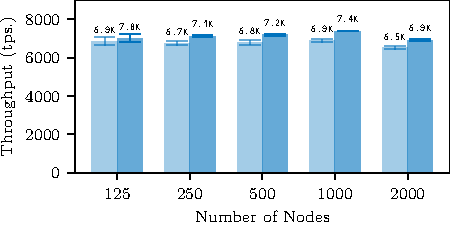
\includegraphics[width=\linewidth]{figures/thr-ava.pdf}
\captionof{figure}{Débit transactionnel en fonction de la taille du réseau. Chaque paire de barres est produite avec
une taille de batch de 20 et 40, de gauche à droite.}
\label{fig:eval-thr}
\end{figure}

\begin{figure}
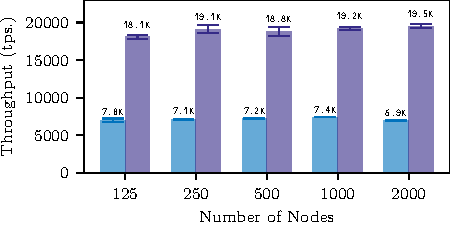
\includegraphics[width=\linewidth]{figures/thr-raw.pdf}
\captionof{figure}{Débit transactionnel pour une taille de batch de 40, avec (gauche) et sans (droite) vérification
de la signature.}
\label{fig:eval-thr-raw}
\end{figure}

\subsection{Mise à l'échelle}

Afin d'observer la manière dont le système passe à l'échelle en terme de nombre de noeuds participant au consensus
{\sysname}, nous effectuons des expériences en gardant des paramètres identiques tout en faisant varier le
nombre de noeuds de 125 jusqu'à 2000.

La Figure~\ref{fig:eval-thr} montre que le débit global se dégrade d'environ $1.34\%$ à 6909 tps lorsque le
réseau augmente d'un facteur 16 pour atteindre $n = 2000$. Cette dégradation est mineure si on la compare au
taux d'augmentation du réseau. Notez que l'axe X est logarithmique.

Avalanche tire sa bonne mise à l'échelle de plusieurs sources\,: premièrement en maintenant un ordre partiel qui
capture uniquement les relations entre les dépenses ce qui permet une meilleure parallélisation qu'un journal
BFT répliqué classique qui traite toutes les transactions de manière linéaire\,; deuxièmement l'absence de dirigeant
permet d'éviter les goulets d'étranglement\,; et finalement le nombre de messages que chaque noeud doit gérer par
décision est $O(k)$ et n'augmente pas au fur et à mesure que le réseau s'agrandit.

\subsection{Engorgement dû à la cryptographie}

Nous examinons ensuite où se situent les goulets d'étranglement dans notre implémentation.
La barre violette à la droite de chaque groupe dans la Figure~\ref{fig:eval-thr-raw} montre le débit
d'Avalanche lorsque la vérification des signatures est désactivée. Les débits s'améliorent d'environ 2.6x, par
par rapport à la barre bleue sur la gauche.
Cela révèle que le surplus de calcul dû à la vérification cryptographique est le principal goulet d'étranglement
de l'implémentation de notre système. On peut pallier ce problème en déléguant la vérification des transactions
à un GPU\@. Même en l'absence d'une telle optimisation, 7K tps dépasse de loin ce qui existe en matière de blockchain.

\subsection{Latence}

\begin{figure}
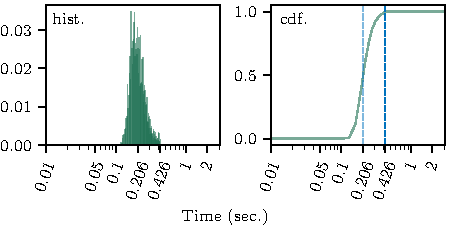
\includegraphics[width=\linewidth]{figures/lat.pdf}
\captionof{figure}{Distribution de la latence de transaction pour $n = 2000$. L'axe X représente la latence
    de transaction en secondes sur une échelle logarithmique, tandis que l'axe Y est la portion des transactions
    qui tombe dans la période de confirmation (normalisée à $1$). L'histogramme de toutes les latences de transaction
    pour un client est visible sur la gauche avec $100$ bins, et son CDF visible sur la droite.}
\label{fig:eval-lat1}
\end{figure}

La latence d'une transaction est le temps écoulé à partir du moment où elle est soumise au réseau jusqu'à ce qu'elle
soit confirmée et donc acceptée par le réseau.

La Figure~\ref{fig:eval-lat1} représente un histogramme montrant la distribution des latences en utilisant la
même configuration que pour les mesures de débits à partir de 2000 noeuds. L'axe X représente le temps en secondes
tandis que l'axe Y est la portion des transactions qui sont finalisées dans la période de temps correspondante.
Cette figure met également en avant la Fonction de Distribution Cumulée (CDF) en accumulant le nombre de
transactions finalisées sur la période.

Cette expérience démontre que la plupart des transactions sont confirmées en moins de 0.3 secondes environ.
La majorité des latences se trouve aux alentours des 206 ms avec une variance relativement faible, ce qui
indique que les noeuds convergent sur la décision finale en tant que groupe environ au même moment. La deuxième
ligne verticale montre la latence maximale observée, qui se situe aux alentours des 0.4 secondes.

La Figure~\ref{fig:eval-lat2} montre la latence de transaction pour un nombre variable de noeuds. Les arêtes
horizontales des boîtes représentent respectivement du bas vers le haut le minimum, le premier quartile, la médiane,
le troisième quartile, et le maximum de latence. En définitive, les données expérimentales montrent que la latence
médiane est plus ou moins indépendante de la taille du réseau.

\begin{figure}[h]
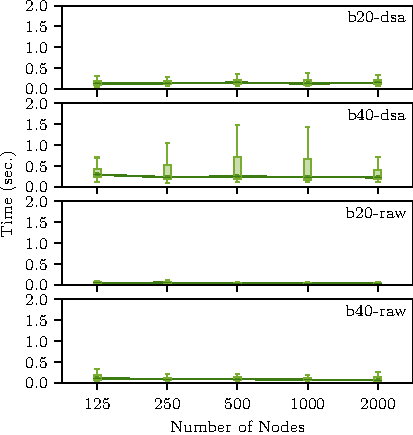
\includegraphics[width=\linewidth]{figures/lat2.pdf}
\captionof{figure}{Latence de transaction en fonction de la taille du réseau. ``b'' indique la taille de batch et
``raw'' est l'occurence sans la vérification des signatures.}
\label{fig:eval-lat2}
\end{figure}

\subsection{Clients malveillants}
\label{sec:evaluation-misbehaving}
\begin{figure}
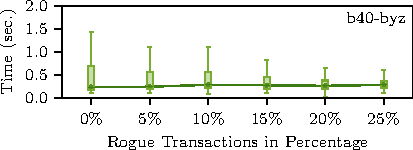
\includegraphics[width=\linewidth]{figures/lat3.pdf}
\captionof{figure}{Latence en fonction du taux de transactions malveillantes.}
\label{fig:eval-lat3}
\end{figure}

Nous évaluons ensuite comment des transactions conflictuelles générées par des clients malveillants effectuant des
double dépenses sur des sorties non dépensées peuvent affecter la latence des transactions légitimes créées par
des clients honnêtes. Nous adoptons une stratégie qui simule des clients malveillants où une fraction (de $0\%$ à $25\%$)
des transactions en attente sont en conflit avec d'autres transactions existantes.

Le processus client effectue ceci en désignant des flux de transactions contenant des double dépenses parmi toutes
les transactions simulées en attente, et envoie les transactions conflictuelles vers différents noeuds. Nous utilisons
pour cela les mêmes paramètres avec $n = 1000$ comme dans les expériences précédentes, et nous mesurons uniquement
le débit et la latence des transactions confirmées.

La latence d'{\sysname} est seulement légèrement influencée par les clients malveillants, comme le montre la
Figure~\ref{fig:eval-lat3}. Étonnamment, la latence maximale baisse légèrement lorsque le pourcentage de transactions
conflictuelles augmente. Ce comportement s'explique par le fait que lorsqu'on introduit de telles transactions, le débit
\emph{effectif} est réduit et soulage donc la charge du système.

Cette observation est confirmée par la figure~\ref{fig:eval-thr2} qui montre que le débit (de transactions légitimes)
decroît avec le taux de transactions conflictuelles. De plus, la baisse du débit apparaît proportionnelle au nombre de
clients malveillants, ce qui démontre que les attaques potentielles ne bénéficient pas d'un effet de levier.

\begin{figure}
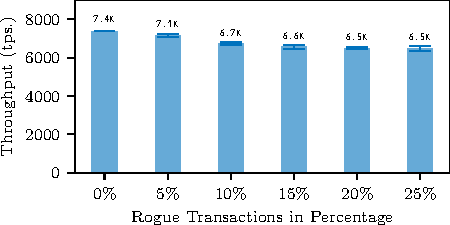
\includegraphics[width=\linewidth]{figures/thr-byz.pdf}
\captionof{figure}{Débit de transactions en fonction du taux de transactions conflictuelles.}
\label{fig:eval-thr2}
\end{figure}

\subsection{Géo-réplication}

\begin{figure}
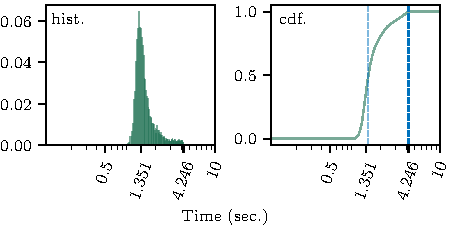
\includegraphics[width=\linewidth]{figures/lat4.pdf}
\captionof{figure}{Histogramme de latence/CDF pour $n = 2000$ réparties dans 20 villes.}
\label{fig:eval-lat4}
\end{figure}

L'expérience suivante place le système dans l'émulation d'un scénario géo-répliqué, modélisé sur le même scénario
détaillé dans un travail préliminaire~\cite{GiladHMVZ17}.
Nous avons sélectionné 20 villes majeures qui semblent être localisées à proximité d'un nombre conséquent de noeuds
Bitcoin joignables, d'après ~\cite{bitnodes2018}. Ces villes couvrent l'Amérique du Nord, l'Europe, l'Asie occidentale,
l'Asie orientale, l'Océanie, et incluent également les 10 villes où l'on trouve le plus grand nombre de noeuds
joignables. Nous utilisons les données de latence obtenues depuis~\cite{wondernetworkping2018} et nous émulons
la latence des paquets réseau dans le noyau Linux en utilisant les commandes \texttt{tc} et \texttt{netem}.
2000 noeuds sont distribués équitablement parmi toutes les villes, sans émuler de latence supplémentaire entre les
noeuds d'une même ville. Comme pour l'évaluation d'Algorand, nous limitons aussi la bande passante par processus
à 20 mégabits par seconde dans le but de simuler des paramètres à l'échelle d'internet d'un réseau comportant de
nombreux liens. Nous assignons ensuite un processus client à chaque ville, qui génère 400 transactions sortantes
par ville à tout moment.

Dans ce scénario, Avalanche atteint un débit de transactions moyen de 3401 tps, avec un écart type de 39 tps. Comme
le montre la Figure~\ref{fig:eval-lat4}, la latence de transaction médiane est de 1.35 secondes, avec une latence
maximale de 4.25 secondes. Nous supportons également le code initial de Bitcoin pour les transactions, qui dans ce
cas donne un débit de 3530 tps avec $\sigma = 92$ tps.

\subsection{Comparaison avec d'autres systèmes}

Même s'il existe une abondance de protocoles blockchain et de cryptomonnaies, la plupart d'entre eux présentent
une ébauche de leur protocole sans proposer d'implémentation pratique ou de résultats d'évaluation. En outre, parmi
ceux qui proposent effectivement des résultats, la plupart ne sont pas évalués dans des conditions réalistes ou à
grande échelle (des centaines de milliers de noeuds complets participant au consensus).

En conséquent, nous choisissons Algorand et Conflux pour notre étude comparative. Algorand, Conflux et Avalanche
sont tous fondamentalement différents dans leur conception. L'algorithme de consensus par comité
d'Algorand repose sur un accord byzantin basé sur un quorum, et Conflux supplémente le consensus de Nakamoto par une
structure de type Graphe Acyclique Orienté (DAG) pour permettre un meilleur débit, tandis qu'Avalanche appartient à
une nouvelle famille de protocoles basés sur la méta-stabilité. Par ailleurs, nous utilisons
Bitcoin~\cite{nakamoto2008bitcoin} comme base technique.

Les évaluations d'Algorand et d'Avalanche reposent toutes deux sur un réseau décisionnel de 2000 noeuds sur EC2.
Notre évaluation se fait sur des instances \texttt{c5.large} partagées, tandis qu'Algorand utilise des instances
\texttt{m4.2xlarge}\@. Ces deux plateformes sont très similaires à l'exception d'un léger avantage en terme de
fréquence CPU pour le \texttt{c5.large}, qui au final n'est que partiellement utilisé puisque nos processus ne
consomment que $30\%$ de temps processeur lors de ces expériences. Les paramètres de sécurité choisis pour nos
expériences garantissent une probabilité de violation de sécurité en dessous de $10^{-9}$ en présence de
$20\%$ de noeuds byzantins, en comparaison de l'évaluation Algorand qui garantit une probabilité de violation en dessous
de $5 \times 10^{-9}$ avec $20\%$ de noeuds byzantins.

Ni Algorand ni Conflux ne prennent en compte le surplus de calcul lié à la vérification cryptographique dans leurs
études. Leurs évaluations utilisent des blocs qui contiennent des mégaoctets de données factices et présentent les
mesures de débit en mégaoctets ou gigaoctets par heure. Nous utilisons donc la taille moyenne d'une transaction
Bitcoin, 250 octets, pour en déduire leurs débits de transactions. Par contraste, nos expériences transportent des
données de transactions réelles et prennent entièrement en compte le temps de calcul des vérifications cryptographiques.

Le débit de transactions est de 3-7 tps pour Bitcoin, 874 tps pour Algorand (avec des blocs de 10 mégaoctets), 3355 tps
pour Conflux (le papier fait mention d'un débit 3.84 fois supérieur au débit d'Algorand dans les mêmes conditions).

En comparaison, {\sysname} obtient constamment plus de 3400 tps sur un réseau allant jusqu'à 2000 noeuds
sans aucun comité de décision ni preuve de travail. Pour ce qui est de la latence, une transaction est confirmée
après 10--60 minutes pour Bitcoin, environ 50 secondes pour Algorand, 7.6--13.8 minutes avec Conflux, et 1.35 secondes
pour {\sysname}.

Avalanche se comporte bien mieux qu'Algorand à la fois en terme de débit et de latence étant donné qu'Algorand utilise une
fonction aléatoire vérifiable pour élire ses comités, et maintient un journal ordonné pendant qu'{\sysname} établit
un ordre partiel uniquement. Bien que l'entité à la tête d'Algorand soit anonyme et change continuellement, elle reste
néanmoins basée sur un dirigeant unique qui pourrait être un facteur limitant pour le passage à l'échelle, tandis
qu'{\sysname} n'est pas contrôlé par une entité unique.

Avalanche a un débit similaire à Conflux, mais sa latence est 337--613 fois meilleure. Conflux utilise également une
structure DAG pour amortir le coût du consensus et augmenter le débit de transactions, cependant il est toujours ancré
sur un consensus de Nakamoto (PoW) le rendant incapable de confirmer des transactions instantanément comme le fait
Avalanche.

Dans un système à base de blockchain, on ne peut généralement améliorer le débit des transactions qu'aux dépens de la
latence à travers le regroupement par batchs. Le vrai facteur limitant au niveau de la performance est le nombre de
décisions qu'un système est en mesure de prendre en une seconde, et ce paramètre est fondamentalement limité soit par
l'accord byzantin ($\mathrm{BA}^{*}$) chez Algorand soit par le consensus de Nakamoto pour Conflux.



\section{Travaux associés}
\label{sec:related-work}
\label{section:background}
\tronly{
Bitcoin~\cite{nakamoto2008bitcoin} est une cryptomonnaie qui utilise une blockchain basée sur la preuve de travail
(PoW pour "Proof Of Work") et qui tient un livre de comptes des "sorties de transaction non dépensées", ou UTXO
("Unspent Transaction Output") en anglais. Bien que des techniques basées sur la preuve de
travail~\cite{DworkN92, aspnes2005exposing}, et même d'autres cryptomonnaies dont la génération de pièces est basée
sur la preuve de travail~\cite{vishnumurthy2003karma,rivest1997payword}, ont été explorées avant l'apparition de
Bitcoin, ce dernier fut le premier à incorporer la preuve de travail dans son processus de consensus. Contrairement
aux protocoles résistants aux fautes byzantines traditionnels, Bitcoin apporte une garantie de sûreté probabiliste et
considère que la majorité de la puissance de calcul agit de manière honnête plutôt que de contrôler les membres du
réseau, ce qui a permis de faire émerger un protocole sans permission à l'échelle d'internet. Bien qu'il soit sans
permission et résilient face aux attaques, Bitcoin souffre d'un débit de transaction faible (\textasciitilde{}3 tps)
et d'une latence élevée (\textasciitilde{}5.6 heures pour un réseau comportant 20\% de noeuds byzantins et une garantie
de sûreté de $2^{-32}$). De plus la preuve de travail nécéssite une puissance de calcul considérable qui est consommée
dans le seul et unique but de maintenir la sûreté de fonctionnement.

%0 Bitcoin~\cite{nakamoto2008bitcoin} is a cryptocurrency that uses a blockchain based on
%0 proof-of-work (PoW) to maintain a ledger of UTXO transactions.
%0 While techniques based on proof-of-work~\cite{DworkN92, aspnes2005exposing}, and even cryptocurrencies with minting based on proof-of-work~\cite{vishnumurthy2003karma,rivest1997payword}, have been explored before, Bitcoin was the first to incorporate PoW into its consensus process.
%0 Unlike more traditional BFT protocols, Bitcoin has a probabilistic safety guarantee
%0 and assumes honest majority computational power rather than a known
%0 membership, which in turn has enabled an internet-scale permissionless protocol. While permissionless and resilient to adversaries,
%0 Bitcoin suffers from low throughput (\textasciitilde{}3 tps) and
%0 high latency (\textasciitilde{}5.6 hours for a network with 20\% Byzantine presence and $2^{-32}$ security guarantee).  Furthermore, PoW requires a substantial amount of computational power that is consumed only for the purpose of maintaining
%0 safety.

D'innombrables cryptomonnaies utilisent la preuve de travail~\cite{DworkN92, aspnes2005exposing} dans le but de tenir
un livre de comptes distribué. Tout comme Bitcoin, elles souffrent des mêmes limitations lorsqu'il s'agit de monter en
charge. Il existe plusieurs propositions de protocoles essayant de faire meilleur usage des progrès apportés par la
preuve de travail. Bitcoin-NG~\cite{EyalGSR16} et la version sans permission de Thunderella~\cite{PassS18} utilise
un consensus similaire à celui de Nakamoto pour élire un leader qui va dicter les écritures dans le journal répliqué
pour un temps donné assez long dans le but de fournir un meilleur débit de transactions. En outre, Thunderella apporte
une borne optimiste qui, en considérant 3/4 de puissance de calcul et un leader élu honnêtes, permet de confimer les
transactions rapidement. ByzCoin~\cite{Kokoris-KogiasJ16} sélectionne un échantillon réduit de participants de manière
périodique et exécute ensuite un protocole résistant aux fautes byzantines en pratique (PBFT) entre les noeuds
sélectionnés.

%O % PoW family
%O Countless cryptocurrencies use PoW~\cite{DworkN92, aspnes2005exposing} to maintain a distributed ledger.
%O Like Bitcoin, they suffer from inherent scalability bottlenecks.
%O Several proposals for protocols exist that try to
%O better utilize the effort made by PoW.
%O Bitcoin-NG~\cite{EyalGSR16} and the permissionless version of
%O Thunderella~\cite{PassS18} use Nakamoto-like consensus to elect a leader that
%O dictates writing of the replicated log for a relatively long time so as to
%O provide higher throughput. Moreover, Thunderella provides an
%O optimistic bound that, with 3/4 honest computational power and an honest
%O elected leader, allows transactions to be confirmed rapidly.
%O ByzCoin~\cite{Kokoris-KogiasJ16} periodically selects a small set of
%O participants and then runs a PBFT-like protocol within the selected nodes.
%O %It achieves a throughput of 942 tps with about 35 second latency.

Les protocoles basés sur un accord byzantin~\cite{PeaseSL80, LamportSP82} se basent généralement sur un quorum et
nécéssitent une connaissance précise des membres du réseau. PBFT~\cite{castro1999practical, CL02}, l'un de ces
protocoles les plus connus, nécessite un nombre quadratique d'échanges de messages avant de parvenir à un accord.
Le protocole Q/U~\cite{abd2005fault} et la réplication HQ~\cite{cowling2006hq} utilisent une approche basée sur un
quorum afin d'optimiser le protocole pour obtenir des cas de fonctionnement sans contention et parvenir à un consensus
en un seul tour de communication. Malgré tout, même si ces protocoles améliorent les performances, ils se dégradent
fortement lorsqu'ils sont soumis à une forte contention. Zyzzyva~\cite{KotlaADCW09} ajoute au protocole BFT une
exécution spéculative pour tendre vers un cas de fonctionnement sans erreurs. Les travaux passés portant sur les
systèmes résistants aux fautes byzantines avec contrôle d'accès nécessitent typiquement au moins $f+1$ répliques.
CheapBFT~\cite{kapitza2012cheapbft} tire profit de composants matériels certifiés pour construire un protocole
nécessitant exactement $f+1$ répliques.

%O % Byzantine Agreement family
%O Protocols based on Byzantine agreement~\cite{PeaseSL80, LamportSP82} typically make use of
%O quorums and require precise knowledge of membership.
%O PBFT~\cite{castro1999practical, CL02}, a well-known representative, requires a quadratic number of message exchanges in order to
%O reach agreement.
%O %Some variants are able to scale to dozens of nodes~\cite{ClementWADM09, KotlaADCW09}.
%O The Q/U protocol~\cite{abd2005fault} and HQ replication~\cite{cowling2006hq} use a quorum-based approach to optimize for contention-free cases of operation to achieve consensus in only a single round of communication. However, although these protocols improve on performance, they degrade very poorly under contention. Zyzzyva~\cite{KotlaADCW09} couples BFT with speculative execution to improve the failure-free operation case.
%O %Aliph~\cite{guerraoui2010next} introduces a protocol with optimized performance under several, rather than just one, cases of execution. In contrast, Ardvark~\cite{ClementWADM09} sacrifices some performance to tolerate worst-case degradation, providing a more uniform execution profile. This work, in particular, sacrifices failure-free optimizations to provide consistent throughput even at high number of failures.
%O Past work in permissioned BFT systems typically requires at least $3f+1$ replicas. CheapBFT~\cite{kapitza2012cheapbft} leverages trusted hardware components to construct a protocol that uses $f+1$ replicas.

D'autres travaux tentent d'introduire de nouveaux protocoles qui redéfinissent et relâchent les contraintes du modèle
de résistance aux fautes byzantines. La résistance byzantine à grande échelle~\cite{rodrigues2007large} modifie la
résistance byzantine pratique (PBFT) pour autoriser un nombre arbitraire de répliques et un seuil d'échec, en
fournissant une garantie de vitalité probabilitse pour un taux d'échec donné tout en protégeant la sûreté de
fonctionnement avec une probabilité élevée. Dans une autre forme de relâchement des contraintes,
Zeno~\cite{singh2009zeno} introduit un protocole de réplication de machine d'état résistante aux fautes byzantines qui
échange la cohérence pour une meilleure disponibilité. Plus spécifiquement, Zeno garantit une cohérence assurée au final
plutôt qu'une linéarisation de celle-ci, ce qui veut dire que les participants n'ont pas besoin d'être conhérents mais
doivent se mettrent d'accord au final une fois le réseau stabilisé. En fournissant une garantie de cohérence encore
plus faible, appelée "cohérence causale par embranchement-raccord", Depot~\cite{mahajan2011depot} définit un protocole
garantissant la sûreté de fonctionnement pour $2f+1$ répliques.

NOW~\cite{guerraoui2013highly} uttilise des sous-quorums pour diriger des instances de consensus réduites.
L'enseignement de ce papier est que de petits quorums de taille logarithmique peuvent être extraits à partir d'un
échantillon potentiellement large de noeuds du réseau, ce qui permet à des instances de protocole de consensus plus
petites de tourner en parallèle.

Snow White~\cite{cryptoeprint:2016:919} et Ouroboros~\cite{KiayiasRDO17} font partie des premiers protocoles à la
sûreté prouvée basés sur la preuve d'enjeu (PoS - ou "Proof Of Stake" en anglais). Ouroboros utilise un protocole de
bascule de jeton multi-parties sécurisé dans le but d'incorporer un caractère aléatoire dans l'élection du leader.
Son évolution Ouroboros Praos~\cite{DavidGKR18} apporte la sûreté en présence d'attaquants entièrement adaptatifs.
HoneyBadger~\cite{MillerXCSS16} démontre une bonne vitalité dans un réseau comportant des latences hétérogènes.

Tendermint~\cite{buchman2016tendermint, 1807.04938} change de leader à chaque bloc et a démontré ses qualités dans une
configuration à 64 noeuds. Ripple~\cite{schwartz2014ripple} a une faible latence grâce à l'utilisation de sous-réseaux
certifiés collectivement au sein d'un réseau plus large. La société Ripple génère une liste de noeuds vérifiés par
défaut renouvelée peu souvent, qui en fait un réseau essentiellement centralisé.

HotStuff~\cite{hotstuff,hotstuffpodc} améliore les coûts de communication d'une distribution quadratique vers une
distribution linéaire et simplifie drastiquement les caractéristiques du protocole, même si les limitations liées
à l'élection d'un leader persistent. Facebook utilise Hotstuff comme le consensus principal de son projet Libra.

Dans une configuration synchrone, inspirée par Hoststuff, Sync HotStuff~\cite{synchotstuff} atteint un consensus en
un temps $2\Delta$ avec un coût quadratique et contrairement à d'autres protocoles synchrones à étapes vérouillées, il
opère aussi rapidement que le réseau se propage. Stellar~\cite{mazieres2015stellar} se base sur un accord byzantin
fédéré dans lequel des \emph{tranches de quorum} permettent une confiance hétérogène entre des noeuds différents. La
sûreté de fonctionnement est garantie lorsque les transactions peuvent être reliées entre elles de manière transitive
par des tranches de quorum. Algorand~\cite{GiladHMVZ17} utilise une fonction aléatoire vérifiable pour sélectionner un
comité de noeuds qui participent à un protocole de consensus byzantin innovant.

%0 Other work attempts to introduce new protocols under redefinitions and relaxations of the BFT model.
%0 Large-scale BFT~\cite{rodrigues2007large} modifies PBFT to allow for arbitrary choice of number of replicas and failure threshold, providing a probabilistic guarantee of liveness for some failure ratio but protecting safety with high probability.
%0 In another form of relaxation. Zeno~\cite{singh2009zeno} introduces a BFT state machine replication protocol that trades consistency for high availability. More specifically, Zeno guarantees eventual consistency rather than linearizability, meaning that participants can be inconsistent but eventually agree once the network stabilizes. By providing an even weaker consistency guarantee, namely fork-join-causal consistency, Depot~\cite{mahajan2011depot} describes a protocol that guarantees safety under $2f+1$ replicas.
%0
%0 NOW~\cite{guerraoui2013highly} uses sub-quorums to drive smaller instances of consensus. The insight of this paper is that small, logarithmic-sized quorums can be extracted from a potentially large set of nodes in the network, allowing smaller instances of consensus protocols to be run in parallel.

%O Snow White~\cite{cryptoeprint:2016:919} and
%O Ouroboros~\cite{KiayiasRDO17} are some of the earliest provably secure PoS
%O protocols.  Ouroboros uses a secure multiparty coin-flipping protocol to
%O produce randomness for leader election. The follow-up protocol, Ouroboros
%O Praos~\cite{DavidGKR18} provides safety in the presence of fully adaptive
%O adversaries.
%O HoneyBadger~\cite{MillerXCSS16} provides good liveness in a network with heterogeneous latencies. %and achieves over 819 tps with 5 minute latency on 104 nodes.

%O Tendermint~\cite{buchman2016tendermint, 1807.04938} rotates the leader for each block
%O and has been demonstrated with as many as 64 nodes. Ripple~\cite{schwartz2014ripple} has low latency by utilizing collectively-trusted
%O sub-networks in a large network. The Ripple company provides a
%O slow-changing default list of trusted nodes, which renders the system essentially centralized.
%O HotStuff~\cite{hotstuff,hotstuffpodc} improves the communication cost from quadratic to linear and significantly simplifies the protocol specification, although the leader bottleneck still persists. Facebook uses HotStuff as the core consensus for its Libra project.
%O % Ittai paper
%O In the synchronous setting, inspired by HotStuff, Sync HotStuff~\cite{synchotstuff} achieves consensus in $2\Delta$ time with quadratic cost and unlike other lock-steped synchronous protocols, it operates as fast as network propagates.
%O Stellar~\cite{mazieres2015stellar} uses Federated Byzantine Agreement in which \emph{quorum slices}
%O enable heterogeneous trust for different nodes.  Safety is guaranteed when
%O transactions can be transitively connected by trusted quorum slices.
%O Algorand~\cite{GiladHMVZ17} uses a verifiable random function to select a
%O committee of nodes that participate in a novel Byzantine consensus
%O protocol.
%It achieves over 874 tps with 50 second latency on
%an emulated network of 2000 committee nodes (500K users in total) distributed among 20 cities. To prevent Sybil
%attacks, it uses a mechanism like proof-of-stake that assigns weights to participants in committee selection based on the money in their accounts.

Certains protocoles utilisent une structure de graphe orienté acyclique (DAG) en lieu et place d'une chaîne linéaire
pour atteindre un consensus~\cite{SompolinskyZ15,SompolinskyLZ16,SompolinskyZ18,BentovHMN17,baird2016hashgraph}.
Au lieu de choisir la chaîne la plus longue comme dans Bitcoin, GHOST~\cite{SompolinskyZ15} définit des règles de
sélection de la chaîne qui permettent de prendre en considération des transactions non présentes sur la chaîne
principale, ce qui augmente son efficacité. SPECTRE~\cite{SompolinskyLZ16} utilise des transactions sur le DAG pour
voter de manière récursive via la preuve de travail pour atteindre un consensus, suivi par
SPECTRE~\cite{SompolinskyLZ16} qui obtient un ordre linéaire à partir de tous les blocs. Tout comme PHANTOM, Conflux
obtient également un ordre linéaire entre les transactions via la preuve de travail utilisée sur une structure DAG,
avec une meilleure résistance aux attaques à la vitalité~\cite{confluxLLXLC18}.

Avalanche est différent dans son approche par laquelle le résultat du vote est un reçu instantané déterminé par une
requête sans preuve de travail, tandis que les votes dans PHANTOM ou Conflux sont purement déterminés par la preuve de
travail dans la structure de transactions. A la manière de Thunderella, Meshcash~\cite{BentovHMN17} combine un protocole
lent basé sur la preuve de travail et un protocole de consensus rapide qui apporte une fréquence de génération de blocs
élevée quelque soit la latence du réseau, offrant un temps de confirmation rapide. Hashgraph~\cite{baird2016hashgraph}
est un protocole sans leader qui construit un DAG sur la base d'un "bavardage rendu aléatoire". Il nécessite une
connaissance complète des membres du réseau à tout moment, et comme Ben-Or~\cite{ben1983another}, il s'attend à un
nombre de messages exponentiel~\cite{aspnes2003randomized,CachinV17} pour fonctionner.

%O Some protocols use a Directed Acyclic Graph (DAG) structure instead of a linear chain to achieve
%O consensus~\cite{SompolinskyZ15,SompolinskyLZ16,SompolinskyZ18,BentovHMN17,baird2016hashgraph}.
%O Instead of choosing the longest chain as in Bitcoin,
%O GHOST~\cite{SompolinskyZ15} uses a more efficient chain selection rule that
%O allows transactions not on the main chain to be taken into consideration, increasing efficiency.
%O SPECTRE~\cite{SompolinskyLZ16} uses transactions on
%O the DAG to vote recursively with PoW to achieve consensus, followed up by
%O PHANTOM~\cite{SompolinskyZ18} that achieves a linear order among all blocks.
%O Like PHANTOM, Conflux also finalizes a linear order of transactions by PoW
%O in a DAG structure, with better resistance to liveness attack~\cite{confluxLLXLC18}.
%O Avalanche
%O is different in that the voting result is a one-time chit that is determined by
%O a query without PoW, while the votes in PHANTOM or Conflux are purely determined by PoW in transaction structure.
%O Similar to Thunderella, Meshcash~\cite{BentovHMN17} combines a slow PoW-based protocol with a fast consensus protocol that allows a high block rate regardless of network latency, offering fast confirmation time.
%O Hashgraph~\cite{baird2016hashgraph} is a leader-less protocol that builds a DAG via randomized gossip.
%O It requires full membership knowledge at all times, and, similar to the Ben-Or~\cite{ben1983another}, it requires exponential messages~\cite{aspnes2003randomized,CachinV17} in expectation.
}{
% PoW family
Several proposals for protocols exist that try to
better utilize the effort made by PoW.
Bitcoin-NG~\cite{EyalGSR16} and the permissionless version of
Thunderella~\cite{PassS18} use Nakamoto consensus to elect a leader that
dictates writing of the replicated log for a relatively long time so as to
provide higher throughput. Moreover, Thunderella provides an
optimistic bound that, with 3/4 honest computational power and an honest
elected leader, allows transactions to be confirmed rapidly.
ByzCoin~\cite{Kokoris-KogiasJ16} periodically selects a small set of
participants and then runs a PBFT-like protocol within the selected nodes. 
%It achieves a throughput of 942 tps with about 35 second latency.

% Byzantine Agreement family
Protocols based on Byzantine agreement~\cite{PeaseSL80, LamportSP82} typically make use of
quorums and require precise knowledge of membership.
PBFT~\cite{castro1999practical, CL02}, a well-known representative, requires a quadratic number of message exchanges in order to
reach agreement. Some variants are able to scale to dozens of nodes~\cite{ClementWADM09, KotlaADCW09}.
% However, due to the quadratic message complexity, many variants based on PBFT also inherit this scalability issue.
Snow White~\cite{cryptoeprint:2016:919} and
Ouroboros~\cite{KiayiasRDO17} are some of the earliest provably secure PoS
protocols.  Ouroboros uses a secure multiparty coin-flipping protocol to
produce randomness for leader election. The follow-up protocol, Ouroboros
Praos~\cite{DavidGKR18} provides safety in the presence of fully adaptive
adversaries.
HoneyBadger~\cite{MillerXCSS16} provides good liveness in a network with heterogeneous latencies. %and achieves over 819 tps with 5 minute latency on 104 nodes.
Tendermint~\cite{buchman2016tendermint, 1807.04938} rotates the leader for each block
and has been demonstrated with as many as 64 nodes. Ripple~\cite{schwartz2014ripple} has low latency by utilizing collectively-trusted
sub-networks in a large network. The Ripple company provides a
slow-changing default list of trusted nodes, which renders the system essentially centralized.
HotStuff~\cite{hotstuff,hotstuffpodc} improves the communication cost from quadratic to linear and significantly simplifies the protocol specification, although the leader bottleneck still persists. Facebook uses HotStuff as the core consensus~\cite{librabft} for the Libra project.
% Ittai paper
In the synchronous setting, inspired by HotStuff, Sync HotStuff~\cite{synchotstuff} achieves consensus in $2\Delta$ time with quadratic cost and unlike other lock-steped synchronous protocols, it operates as fast as network propagates.
Stellar~\cite{mazieres2015stellar} uses Federated Byzantine Agreement in which \emph{quorum slices}
enable heterogeneous trust for different nodes.  Safety is guaranteed when
transactions can be transitively connected by trusted quorum slices.

Some protocols use a Directed Acyclic Graph (DAG) structure instead of a linear chain to achieve
consensus~\cite{SompolinskyZ15,SompolinskyLZ16,SompolinskyZ18,BentovHMN17,baird2016hashgraph}.
Instead of choosing the longest chain as in Bitcoin,
GHOST~\cite{SompolinskyZ15} uses a more efficient chain selection rule that
allows transactions not on the main chain to be taken into consideration, increasing efficiency.
SPECTRE~\cite{SompolinskyLZ16} uses transactions on
the DAG to vote recursively with PoW to achieve consensus, followed up by
PHANTOM~\cite{SompolinskyZ18} that achieves a linear order among all blocks.
Avalanche
is different in that the voting result is a one-time chit that is determined by
a query without PoW, while the votes in PHANTOM are purely determined by transaction structure.
Similar to Thunderella, Meshcash~\cite{BentovHMN17} combines a slow PoW-based protocol with a fast consensus protocol that allows a high block rate regardless of network latency, offering fast confirmation time.
Hashgraph~\cite{baird2016hashgraph} is a leader-less protocol that builds a DAG via randomized gossip. 
It requires full membership knowledge at all times, and, similar to the Ben-Or~\cite{ben1983another}, it requires exponential messages~\cite{aspnes2003randomized,CachinV17} in expectation.
}

\begin{comment}
Moreover, in Theorem 5.16, the author mentions if
there is no supermajority virtual vote, all honest nodes will randomly choose
their votes for the next round. Then with non-zero probability, they could
choose the same vote.  The rounds are repeated until all honest nodes
eventually reach the same vote by chance.  This means as the total number of
nodes increases in Hashgraph, the probability of reaching the same vote in a
single trial drops exponentially due to the random voting~\cite{CachinV17}.
\end{comment}
%The paper does not discuss how many rounds of voting are needed in expectation,
%nor\ \ have we been able to obtain open-source code to evaluate Hashgraph.

%\tronly{
%Instead of voting blindly and relying on randomness
%for each agreement, Avalanche creates a positive feedback where votes are
%collected in a separate k-query process determined by current preference
%established locally on each node over time.  We have demonstrated that
%Avalanche is scalable to 2000 nodes distributed world-wide.
%
%The central component of Avalanche is a
%repeated k-query, which serves both as a probabilistic
%broadcast and as a basis for Byzantine agreement.
%As an optimization, these repeated queries are linked
%together via an artificial DAG structure that amortizes the repeated cost of
%querying.  Avalanche does not require overlapping quorums and
%achieves probabilistic consensus with
%$O(kN)$ overall message complexity instead of quadratic
%while allowing for a degree of network churn.
%}

% XXX ADD SAM TOUEG https://zoo.cs.yale.edu/classes/cs426/2017/bib/bracha85asynchronous.pdf


\section{Conclusion}
\label{sec:conclusions}
%O This paper introduced a novel family of consensus protocols, coupled with the appropriate mathematical tools for analyzing them.
Cet article a présenté une nouvelle famille de protocoles de consensus, accompagnée des outils mathématiques appropriés pour leur analyse.
%O \tronly{These protocols are highly efficient and robust, combining the best features of classical and Nakamoto consensus.}
\tronly{Ces protocoles sont extrêmement efficaces et robustes, et rassemblent les meilleures fonctionnalités des consensus classiques et Nakamoto.}{} 
%O They scale well, achieve high throughput and quick finality, work without precise membership knowledge, and degrade gracefully under catastrophic adversarial attacks.
Ils passent bien à l'échelle, permettent un haut débit et une finalité rapide, ne nécessitent pas une connaissance précise des participants et leur fonctionnement se dégrade progressivement lors d'attaques catastrophiques.

%O There is much work to do to improve this line of research. \tronly{
Il reste beaucoup à faire dans ce domaine de recherche. \tronly{
%O One such improvement could be the introduction of an adversarial network scheduler.
Une amélioration possible consisterait à introduire un coordinateur d'attaques sur le réseau.
%O Another}{One} improvement would be to characterize the system's guarantees under an adversary whose powers are realistically limited, whereupon performance would improve even further. \tronly{Finally, more}{More} sophisticated initialization mechanisms would bear fruitful in improving liveness of multi-value consensus.
Une autre}{Une} serait de caractériser les garanties du système face à un adversaire dont les pouvoirs seraient limités de manière réaliste, à la suite de quoi les performances se verraient encode améliorées. \tronly{D'autres}{Plus} mécanismes d'initialisation sophistiqués seraient souhaitables pour améliorer la vitalité d'un consensus multi-valeurs. 
%O Overall, we hope that the protocols and analysis techniques presented here add to the arsenal of the distributed system developers and provide a foundation for new lightweight and scalable mechanisms.
En résumé, nous espérons que les protocoles et les techniques d'analyse présentés ici renforceront l'arsenal des développeurs de systèmes distribués et permettront de bâtir de nouveaux mécanismes légers et évolutifs.

%\section*{Acknowledgments}\tronly{}{\vspace{-0.5em}}
%\label{sec:related-work}
%We are grateful to the many individuals who provided feedback on earlier drafts. 
% Bobby Kleinberg, Vitalik Buterin, ...

%latex here should be the name of your bibtex file minus '.bib'
%\clearpage
\bibliographystyle{acm}
\bibliography{paper}
%\newpage
\begin{appendices}
%O \section{Analysis}
\section{Analyse}
\label{sec:full-analysis}
%O In this appendix, we provide an analysis of Slush, Snowflake and Snowball.
Cette annexe contient une analyse de Slush, Snowflake et Snowball.
%For lack of space, we leave additional details to an accompanying report.

%O \subsection{Preliminaries}
\subsection{Préliminaires}
%O We assume the network model as discussed in Section~\ref{sec:model_and_goals}. We let $\mathtt{R}$ (``red'') and $\mathtt{B}$ (``blue'') represent two generic conflicting choices.
Nous supposons le modèle réseau discuté en section~\ref{sec:model_and_goals}. Soient $\mathtt{R}$ (``rouge'') et $\mathtt{B}$ (``bleu'') représentant deux choix conflictuels génériques.
%O Without loss of generality, we focus our attention on counts of $\mathtt{B}$, i.e.\ the total number of nodes that prefer blue.
Sans perdre en généralité, nous portons notre attention sur les décomptes de $\mathtt{B}$, c'est-à-dire le nombre de nœuds qui préfèrent le bleu.

%O \paragraph{Hypergeometric Distribution} Each network query of $k$ peers corresponds to a sample without replacement out of a network of $n$ nodes, also referred to as a hypergeometric sample.
\paragraph{Distribution hypergéométrique} Chaque requête réseau de $k$ pairs correspond à un échantillon sans remplacement depuis un réseau de $n$ nœuds, également appelé un échantillon hypergéométrique.
%O We let the random variable $\mathcal{H}(\mathcal{N}, x, k) \rightarrow \{0, \dots, k\}$ denote the resulting counts of $\mathtt{B}$ in the sample (unless otherwise stated), where $x$ is the total count of $\mathtt{B}$ in the population. The probability that the query achieves the required threshold of $\alpha$ or more votes is given by:
La variable aléatoire $\mathcal{H}(\mathcal{N}, x, k) \rightarrow \{0, \dots, k\}$ note les décomptes résultant de $\mathtt{B}$ dans l'échantillon (sauf mention spécifique), où $x$ est le nombre total de $\mathtt{B}$ dans la population. La probabilité que la requête atteigne le seuil requis d'au moins $\alpha$ votes est donnée par :
\begin{equation}
\small
P(\mathcal{H}(\mathcal{N}, x, k) \geq \alpha) = \left.\sum_{j = \alpha}^{k} {x \choose j} {n - x \choose k - j} \middle/ {n \choose k}\right.
\label{eq:hypergeometric}
\end{equation}
%O For ease of notation, we overload $\mathcal{H}(*)$ by implicitly referring to $P(\mathcal{H}(\mathcal{N}, x, k) \geq \alpha)$ as $\mathcal{H}(\mathcal{N}, x, k, \alpha)$. 
Pour faciliter la notation, nous surchargeons $\mathcal{H}(*)$ en nous référant implicitement à $P(\mathcal{H}(\mathcal{N}, x, k) \geq \alpha)$ par $\mathcal{H}(\mathcal{N}, x, k, \alpha)$.

%O \paragraph{Tail Bounds On Hypergeometric Distribution} We can reduce some of the complexity in Equation~\ref{eq:hypergeometric} by introducing a bound on the hypergeometric distribution induced by $\mathcal{H}^k_{\mathcal{N},x}$.
\paragraph{Bornes de queue sur la distribution hypergéométrique} Nous pouvons un peu réduire la complexité de l'équation~\ref{eq:hypergeometric} en introduisant une borne sur la distribution hypergéométrique induite par $\mathcal{H}^k_{\mathcal{N},x}$.
%O Let $p=x/n$ be the ratio of support for $\mathtt{B}$ in the population.
Soit $p=x/n$ la proportion du support pour $\mathtt{B}$ dans la population.
%O The expectation of $\mathcal{H}(\mathcal{N}, x, k)$ is exactly $kp$.
Nous attendons exactement $kp$ pour $\mathcal{H}(\mathcal{N}, x, k)$.
%O Then, the probability that $\mathcal{H}(\mathcal{N}, x, k)$ will deviate from the mean by more than some small constant $\psi$ is given by the Hoeffding tail bound \cite{hoeffding1963probability}, as follows,
Donc, la probabilité que $\mathcal{H}(\mathcal{N}, x, k)$ dévie de la moyenne de plus d'une petite constante $\psi$ est donnée par la borne de queue de Hoeffding~\cite{hoeffding1963probability}, comme suit,
\begin{equation}
\begin{split}
    P(\mathcal{H}(\mathcal{C}, x, k) \leq (p-\psi)k) &\leq e^{-k\mathcal{D}(p-\psi, p)}\\
    &\leq e^{-2(p-\psi)^2k}
\end{split}
\end{equation}
où $\mathcal{D}(p-\psi, p)$ est la divergence de Kullback-Leibler, measurée par
\begin{equation}
\begin{split}
    \mathcal{D}(a, b) &= a \log \frac{a}{b} + (1 - a) \log \frac{1 - a}{1 - b}
\end{split}
\end{equation}

\paragraph{Concentration de sous-martingales}
%O Let $\{X_{\{t \geq 0\}}\}$ be a sub-martingale and $|X_t - X_{t-1}| < c_t$ almost surely. Then, for all positive reals $\psi$ and all positive integers $t$, 
Soit $\{X_{\{t \geq 0\}}\}$ une sous-martingale et $|X_t - X_{t-1}| < c_t$ presque sûrement. Alors, pour tout réel positif $\psi$ et tout entier positif $t$, 
\begin{equation}
\begin{split}
P(X_t \geq X_0 + \psi) \leq e^{-\psi^2 / 2\sum_{i = 1}^{t} c_t^2}
\end{split}
\label{eq:submartingale}
\end{equation}

\subsection{Slush}
%\label{sec:analysis}
%O Slush operates in a non-Byzantine setting; that is, $f = 0$, $c = n$.
Slush opère dans une configuration non-byzantine, c'est-à-dire $f = 0$, $c = n$.
%O In this section, we will characterize the irreversibility properties of Slush (which appear in Snowflake and Snowball), as well as the precise converge rate distribution. The distribution of of both safety and liveness of Slush translate well to the Byzantine setting.
Dans cette section, nous caractériserons les propriétés d'irréversibilité de Slush (qui apparaissent dans Snowflake et Snowball), ainsi que la distribution de taux de convergence précise. La distribution de la sûreté de fonctionnement et de vitalité de Slush se traduisent bien dans une configuration byzantine.

% \begin{figure}
%     \small
% \begin{algorithmic}[1]
%     \State initialize $u.\codecolor \in \{\texttt{R},\texttt{B}\}$ for all $u\in\mathcal{N}$
%     \For{$t = 1$ to $\phi$}
%         \State $u \assign \Call{sample}{\mathcal{N}, 1}$
%         \State $\mathcal{K} \assign \Call{sample}{\mathcal{N}\backslash u, k}$
%         \State $P \assign \texttt{[}v.\codecolor\quad\textbf{for}\ v \in \mathcal{K}\texttt{]}$
%         \For{$\codecolor' \in \{\texttt{R}, \texttt{B}\}$}
%             \If{$P.\Call{count}{\codecolor'} \ge \alpha$}
%                 \State $u.\codecolor \assign \codecolor'$
%             \EndIf
%         \EndFor
%     \EndFor
% \captionof{figure}{Slush run by a global scheduler.}\label{fig:slush_protocol_simulator}
% \end{algorithmic}
% \end{figure}

%O The procedural version of Slush in Figure~\ref{fig:slush-loop} made use of a parameter $m$, the number of rounds that a node executes Slush queries. 
La version procédurale de Slush en figure~\ref{fig:slush-loop} faisait usage d'un paramètre $m$, le nombre de tours d'un nœud exécutant des requêtes Slush.
% To derive this parameter, we transform the protocol execution from a procedural and concurrent version to one carried out by a scheduler, shown in Figure~\ref{fig:slush_protocol_simulator}.
%O What we ultimately want to extract is the total number of rounds $\phi$ that the scheduler will need to execute in order to guarantee that the entire network is the same color, whp.
Nous voulons en définitive extraire le nombre total de tours $\phi$ que l'ordonnanceur doit exécuter afin de garantir que l'entièreté du réseau se retrouve de la même couleur, ceci avec une forte probabilité.

%O We analyze the system mainly using a continuous time process. Let $\{X_{\{t \geq 0\}}\}$ be a CTMC.
Nous analysons le système en utilisant principalement un processus à temps continu. Soit $\{X_{\{t \geq 0\}}\}$ un processus de Markov à temps continu.
%O The state space $\mathcal{S}$ of the stochastic process is a condensed version of the full configuration space, where each state $\{0, \dots, n\}$ represents the total number of blue nodes in the system. 
L'espace d'état $\mathcal{S}$ du processus stochastique est une version condensée de tout l'espace de configuration, où chaque état $\{0, \dots, n\}$ représente le nombre total de nœuds bleus dans le système.

%O Let $\mathcal{F}_{X_s}$ be the filtration, or the history pertaining to the process, up to time $s$. This process is Markovian and time-homogeneous, conforming to 
Soit $\mathcal{F}_{X_s}$ la filtration, ou l'historique afférent au processus, jusqu'au temps $s$. Ce processus est Markovien et homogène dans le temps, se conformant à
\[
    P\{X_t = j | \mathcal{F}_{X_s}\} = P\{X_t = j | X_s\} = P\{X_t = j | X_0\}    
\]
%O Throughout the paper, we use $Q \equiv (q_{ij}, i, j \in \mathcal{S})$ notation to refer to the infinitesimal generator of the process, where death ($i \rightarrow i-1$) and birth ($i \rightarrow i+1$) rates of configuration transitions are denoted via $\mu_i$ and $\lambda_i$ ($\lambda_ i$ is distinct from the clock parameter $\lambda$, and will be clear from context). These rates are 
Dans cet article, nous utilisons la notation $Q \equiv (q_{ij}, i, j \in \mathcal{S})$ pour nous référer au générateur infinitésimal du processus, où les taux de mort ($i \rightarrow i-1$) et de naissance ($i \rightarrow i+1$) de transitions de configuration sont notées via $\mu_i$, et $\lambda_i$ ($\lambda_ i$ est disctint du paramètre d'horloge $\lambda$ et sera sorti du contexte). Ces taux sont
\[
    \begin{cases}
        \mu_i = i\ \mathcal{H}(\mathcal{N}, c-i, k, \alpha), & \text{for } i \rightarrow i - 1 \\
        \lambda_i = (c-i)\ \mathcal{H}(\mathcal{N}, i, k, \alpha), & \text{for } j \rightarrow i + 1 \\
    \end{cases}
\]
%O for $1\leq i\leq c-1$, and where $i = 0$ and $i = c$ are absorbing. Let $p_{ij}(t)$ refer to the probability of transitioning from state $i$ to $j$ at time $t$. 
pour $1\leq i\leq c-1$, et où $i = 0$ et $i = c$ sont absorbants. Soit $p_{ij}(t)$ une référence à la probabilité de transition de l'état $i$ à $j$ à l'instant $t$.
%O We always assume that 
Nous supposons toujours que
\[
    p_{ij}(t) = 
    \begin{cases}
      \lambda_it + o(t), & \text{pour } j = i + 1 \\
      \mu_it + o(t), & \text{pour } j = i - 1 \\
      1 - (\lambda_i + \mu_i)t + o(t), & \text{pour } j = i \\
      o(t), & \text{sinon }\\
    \end{cases}
\]
%O where all $o(t)$ are uniform in $i$. 
où tous les $o(t)$ sont uniformes en $i$.

%O \paragraph{Irreversibility}
\paragraph{Irréversibilité}
%We now discuss the core results of irreversibility properties of our family of protocols.
%O In Section~\ref{sec:analysis}, we discussed the loose Chvatal bound which provided intuitive understanding into the strong irreversibility dynamics of our core subsampling mechanism. In particular, once the network drifts to some majority value, it tends to revert back with only an exponentially small probability. We compute the closed-form expression for reversibility, and show that it is exponentially small.
En section ~\ref{sec:analysis}, nous avons traité la borne de Chtaval qui fournit une compréhension intuitive de la dynamique de forte irréversibilité au cœur de notre mécanisme de sous-échantillonnage. En particulier, une fois que le réseau tend vers une valeur majoritaire donnée, il ne peut s'inverser qu'avec une probabilité exponentiellement petite. Nous calculons l'expression de forme fermée pour la réversibilité, et nous montrons qu'elle est exponentiellement petite.
\begin{theorem}
\label{theorem:slush_prob_convergence_minority}
%O Let $\xi_\delta$ be the probability of absorption into the all-red state ($s_0$), starting from a drift of $\delta$ (i.e. $\delta$ drift away from $n/2$). Then, assuming $\delta > 1$, 
Soit $\xi_\delta$ la probabilité d'absorption dans l'état totalement rouge ($s_0$), commençant par un drift de $\delta$ (c'est-à-dire que $\delta$ tendent à s'éloigner de $n/2$). Alors, en supposant $\delta > 1$,
\begin{equation}
\xi_\delta = 1 - \ddfrac{\sum_{l = 1}^{\delta} \prod_{i = 1}^{l-1} \mu_i^2 \prod_{j = l}^{n-l}\lambda_j}{2\sum_{l = 1}^{n/2}\prod_{i=1}^{l-1}\mu_i^2\prod_{j=l}^{n-l}\mu_j}
\end{equation}
et
% \begin{equation}
% \xi_\delta - \xi_{\delta+1} = \ddfrac{\mu_1^2\dots\mu_{\delta}^2\lambda_{\delta+1}\dots\lambda_{n-\delta}}{\Phi(\alpha, k, n)}
% \end{equation}
% where $\Phi(\alpha, k, n)$ is a constant dependent on $\alpha$, $k$, and $n$, but otherwise independent of starting configuration. 
\begin{equation}
\begin{split}
\ddfrac{\xi_{\delta} - \xi_{\delta+1}}{\xi_{\delta+1} - \xi_{\delta+2}} &= \mathcal{u}_{\delta+1} = \ddfrac{\lambda_{\delta+1}}{\mu_{\delta+1}} \\
&\approx \ddfrac{n-\delta-1 \sum_{j = \alpha}^{k}\ddfrac{(n-\delta-1)^k (\delta+1)^{k-j}}{n^{2k - j}}}{\delta+1 \sum_{j = \alpha}^{k}\ddfrac{(\delta+1)^k (n-\delta-1)^{k-j}}{n^{2k - j}}}
\end{split}
\end{equation}
%O where from now on we refer to $\mathcal{u}_{\delta+1}$ as the drift of the process. 
où à partir de maintenant nous nous référons à $\mathcal{u}_{\delta+1}$ comme étant le drift du processus.
\end{theorem}

\begin{proof}
%O Our results are derived based on constructions from Tan~\cite{tan1976absorption}. We construct a sub-matrix of $Q$, denoted $B$, as shown in Figure~\ref{fig:matrixB}.
Nos résultats sont dérivés en se fondant sur les constructions de Tan~\cite{tan1976absorption}. Nous construisons une sous-matrice de $Q$, notée $B$, comme on le voit en figure~\ref{fig:matrixB}.
\begin{figure*}
\[B = 
\begin{bmatrix}
    -(\lambda_1 + \mu_1) & \lambda_1 & 0 & \cdots & \cdots & 0 \\
    \mu_2 & -(\lambda_2 + \mu_2) & \lambda_2 & 0 & \cdots & 0\\
    0 & \mu_3 & -(\lambda_3 + \mu_3) & \lambda_3 & \cdots & 0\\
    \vdots & \vdots & \ddots & \ddots & \ddots & \vdots\\
    \vdots & \vdots & \mu_{n-3} & -(\lambda_{n-2} + \mu_{n-2}) & \lambda_{n-3} & 0\\
    \vdots & \dots & 0 & \mu_{n-1} & -(\lambda_{n-2} + \mu_{n-2}) & \lambda_{n-2}\\
    0 & \dots & 0 & 0 & \mu_{n-1} & -(\lambda_{n-1} + \mu_{n-1})
\end{bmatrix}
\]
\caption{Matrice $B$.}
\label{fig:matrixB}
\end{figure*}
%O Let $W_1'$ = $(\mu_1, 0, \dots, 0)$, $W_{n-1}'$ = $(0, \dots, 0, \lambda_{n-1})$. Then, we can express $Q$ as 
Soit $W_1'$ = $(\mu_1, 0, \dots, 0)$, $W_{n-1}'$ = $(0, \dots, 0, \lambda_{n-1})$. Alors nous pouvons exprimer $Q$ par
\[
    Q =
    \begin{bmatrix}
        0 & \dots & 0\\
        W_1 & B & W_{n-1}\\
        0 & \dots & 0
    \end{bmatrix}
\]
%O As a reminder, the stationary distribution can be found via $\lim_{t \rightarrow \infty} P(t) = e^{Qt}$, where we have
Rappelons que la distribution stationnaire peut être trouvée \emph{via} $\lim_{t \rightarrow \infty} P(t) = e^{Qt}$, où nous avons
\[
    e^{Qt} = \sum_{i = 0}^{\infty} \frac{t^i}{i!} Q^i = \sum_{i = 0}^{\infty} \frac{t^i}{i!}
    \begin{bmatrix}
        0 & \dots & 0\\
        B^{i-1}W_1 & B^i & B^{i-1}W_{n-1}\\
        0 & \dots & 0
    \end{bmatrix}
\]
%O As Tan (eq. 2.3) shows, we have
Comme le montre Tan (eq. 2.3), nous avons
\[
    \xi(t) = B^{-1}\left[\sum_{i = 0}^{\infty} B^i  - \mathbb{I}_{n-1} \right] W_1
\]
%O Since we want the ultimate probabilities, we have that 
Comme nous voulons les probabilités ultimes, nous avons 
\[
    \xi = \lim_{t \rightarrow \infty} \xi(t) = -B^{-1}W_1
\]
%O We can explicitly compute $\xi_\delta$ in terms of our rates $\mu_i$ and $\lambda_i$, getting 
Nous pouvons explicitement calculer $\xi_\delta$ en termes de nos taux $\mu_i$ et $\lambda_i$, obtenant ainsi
\[
    \xi_\delta = \ddfrac{\sum_{l = 1}^{n-\delta}\prod_{i = 1}^{n-l}\mu_i \prod_{j = n-l+1}^{n-1}\lambda_j}{\sum_{l = 1}^{n}\prod_{i = 1}^{n-l}\mu_i \prod_{j = n-l+1}^{n-1}\lambda_j}
\]
%O However, we note that $u_{i} = \lambda_{n-i}$. Algebraic manipulation from this observation leads to the two equations in the theorem. This expression is strictly lower than the Chvatal bounds used in Section~\ref{sec:analysis}.
Cependant, notons que $u_{i} = \lambda_{n-i}$. La manipulation algébrique à partir de cette observation mène aux deux équations du théorème. Cette expression est strictement inférieure aux bornes de Chtaval utilisées en section~\ref{sec:analysis}.
\end{proof}

%O Using the construction for the absorption (and (ir)reversibility) probabilities as discussed previously, a natural follow up computation is in regards to \emph{mean convergence time}. 
En utilisant la construction pour les probabilités d'absorption (et d'(ir)réversibilité) précédemment traitées, il est naturel de poursuivre par un calcul concernant le \emph{temps de convergence moyen}.
%O Let $T_{z}(t) = \inf \{t \geq 0 : X_t = \{0, n\} | X_0 = z\}$, and let $\tau_z = \mathbb{E}[T_{z}(t)]$. $\tau_z$ is the mean time to reach either absorbing state, starting from state $z$, which corresponds to the mean convergence time. The next theorem characterizes this distribution.
Soit $T_{z}(t) = \inf \{t \geq 0 : X_t = \{0, n\} | X_0 = z\}$, et soit $\tau_z = \mathbb{E}[T_{z}(t)]$. $\tau_z$ est le temps moyen pour atteindre l'un ou l'autre des états absorbants, à partir de l'état $z$, qui correspond au temps moyen de convergence. Le théorème suivant caractérise cette distribution.

\begin{theorem}
\label{theorem:mean-convergence-time}
%O Let $\tau_z$ be the expected time to convergence, starting from state $z > n/2$, to any of the two converging states in the network (all-red or all-blue). Then, 
Soit $\tau_z$ le temps attendu de convergence, à partir de l'état $z > n/2$, vers l'un des deux états convergents dans le réseau (totalement rouge ou totalement bleu). Alors,
\begin{equation}
\tau_z = \ddfrac{\sum_{d = 1}^{n-1}x(d)y(d)}{2\sum_{l = 1}^{n/2}\prod_{i=1}^{l-1}\mu_i^2\prod_{j=l}^{n-l}\mu_j}
\end{equation}
%O where $x(d)$ and $y(d)$ are
où $x(d)$ et $y(d)$ sont
\begin{equation}
\begin{split}
x(d) &= \sum_{l = 1}^{\min(z, d)} \prod_{i=1}^{l-1} \mu_i \prod_{j = l}^{d-1} \lambda_j\\
y(d) &= \sum_{l = 1}^{n - d - \max(z-d, 0)} \prod_{i = d+1}^{n-l} \mu_i \prod_{j = n - l + 1}^{n - 1} \lambda_j
\end{split}
\end{equation}
\end{theorem}

\begin{proof}
%O Following the calculations from before, $-B^{-1}$ at row $z$ provides the number of traversals to each other state starting from $z$. Calculating their sum, we have our result. The above equation is the full expression of the matrix row sum. 
D'après les calculs qui précèdent, $-B^{-1}$ à la rangée $z$ fournit le nombre de traversées vers chaque autre état en partant de $z$. En calculant leur somme, nous avons notre résultat. L'équation ci-dessus est l'expression complète de la somme des rangées des matrices.
\end{proof}

%O Theorem~\ref{theorem:mean-convergence-time} leads to the next lemma that captures property P2, under the assumption that at the beginning of the protocol, one proposal has at least $\alpha$ support in the network. 
Le théorème~\ref{theorem:mean-convergence-time} mène au lemme suivant qui formalise
la propriété P2, en suppposant qu'au début du protocole, une proposition possède un support d'au moins $\alpha$ dans le réseau.
\begin{lemma}
%O Slush reaches an absorbing state in finite time almost surely.
Slush atteint presque sûrement un état absorbant dans un temps fini.
\label{lemma:finitetermination}
\end{lemma}

\begin{proof}
%O Starting from any non-absorbing, transient state, there is a non-zero probability of being absorbed. Additionally, since termination is finite and everywhere differentiable, Theorem~\ref{theorem:mean-convergence-time} also implies that the probability of termination of any network configuration where a proposal has $\geq \alpha$ support in bounded time $t_{max}$ is strictly positive. 
En partant d'un quelconque état non-absorbant et transitoire, il y a une probabilité non nulle d'absorption. De plus, comme la terminaison est finie et différentiable partout, le théorème~\ref{theorem:mean-convergence-time} implique aussi que la probabilité de terminaison de toute configuration réseau où une proposition a un support $\geq \alpha$ dans un temps borné $t_{max}$ est strictement positive.
\end{proof}

\subsection{Snowflake}
\label{subsection:appendix_snowflake}
%O In Snowflake, the sampled set of nodes includes Byzantine nodes.
Dans Snowflake, l'ensemble des nœuds échantillonnés comprend des nœuds byzantins.
%O We introduce the decision function $\mathcal{D}(*)$, which is constructed by having each node also keep track of the total number of consecutive times it has sampled a majority of the same color ($\beta$). 
Nous introduisons finalement une fonction appelée $\mathcal{A}(\mathcal{S}_t)$ qui est construite en faisant conserver à chaque nœud la trace du nombre total de fois consécutives qu'il a échantillonné une majorité de la couleur d'échantillon ($\beta$).
%O Finally, we introduce a function called $\mathcal{A}(\mathcal{S}_t)$, the adversarial strategy, that takes as parameters the entire configuration of the network at time $t$, as well as the next set of nodes chosen by the scheduler to execute, and as a side-effect, modifies the set of nodes $\mathcal{B}$ to some arbitrary configuration of colors.
Enfin, nous introduisons une fonction appelée $\mathcal{A}(\mathcal{S}_t)$, la stratégie contradictoire, qui prend comme paramètres toute la configuration du réseau à l'instant $t$, ainsi que l'ensemble suivant de nœuds choisi par l'ordonnanceur pour exécution, avec pour effet secondaire la modification de l'ensemble de nœuds $\mathcal{B}$ vers une configuration arbitraire de couleurs.

%O In order for our prior framework to apply to Snowflake, we must deal with a key subtlety. 
Afin d'appliquer notre framework antérieur à Snowflake, nous devons porter notre attention sur une subtilité essentielle.
%O Unlike in Slush, where it is clear that once the network has reached one of the converging states and therefore may not revert back, this no longer applies to Snowflake, since any adversary $f \geq \alpha$ has strictly positive probability of reverting the system, albeit this probability may be infinitesimally small. 
Contrairement à Slush, où il est clair qu'une fois que le réseau a atteint l'un des états convergents et ne reviendra donc pas en arrière, cela ne s'applique pas à Snowflake, puisque tout adversaire $f \geq \alpha$ a une probabilité strictement positive d'inverser la tendance du système, fût-elle infinitésimale.
%O The CTMC is flexible enough to deal with a system where there is only one absorbing state, but the long-term behavior of the system is no longer meaningful since, after an infinite amount of time, the system is guaranteed to revert, violating safety. 
Le processus de Markov à temps continu est assez souple pour s'accommoder d'un système où il n'existe qu'un seul état absorbant, mais le comportement du système sur le long terme n'est plus significatif puisque, après un laps de temps infini, le système doit s'inverser, violant ainsi la sécurité de fonctionnement.
%O We could trivially bound the amount of time, and show safety using this bounded time assumption by simply characterizing the distribution of $e^{tQ}$, where $Q$ is the generator. 
Nous pouvons borner trivialement l'intervalle de temps et montrer la sûreté de fonctionnement grâce à ce bornage en nous contentant de caractériser la distribution de $e^{tQ}$, où $Q$ est le générateur.
%O However, we can make the following observation: if the probability of going from state $c$ (all-blue) to $c-1$ is exponentially small, then it will take the attacker exponential time (in expectation; note, this is a lower bound, and in reality it will take much longer) to succeed in reverting the system. 
Nous pouvons cependant faire l'observation suivante : si la probabilité d'aller de l'état $c$ (totalement bleu) à $c-1$ est exponentiellement petite, alors il faudra à l'attaquant un temps exponentiel (attendu\,; on note que c'est une borne inférieure et, en réalité, il faudra beaucoup plus longtemps) pour réussir à inverser l'état du système.
%O Hence, we can assume that once all correct nodes are the same color, the attack from the adversary will terminate since it is impractical to continue an attack. 
Nous pouvons donc suppposer qu'une fois que tous les nœuds légitimes ont adopté la même couleur, l'attaque de l'adversaire se termine puisqu'il serait irréaliste de la poursuivre.

%O In fact, under reasonably bounded timeframes, the variational distance between the exact approach and the approximation is very small. 
En fait, dans un cadre temporel raisonnablement borné, la distance variationnelle entre l'approche exacte et l'approximation est très petite.
%O We leave details to the accompanying paper, but we briefly discuss how analysis proceeds for Snowflake. 
Nous laissons les détails à l'article qui accompagne celui-ci, mais nous discutons brièvement du déroulement de l'analyse pour Snowflake.


%O As stated in Section~\ref{sec:analysis}, the way to analyze the adversary using the same construction as in Slush is to condition reversibility on the first node $u$ deciding on blue, which can happen at any state (as specified by $\mathcal{D}(*)$). At that point, the adversarial strategy collapses to a single function, which is to continually vote for red. The probabilities of reversibility, for all states $\{1, \dots, c-1\}$ must encode the probability that additional blue nodes commit, and the single function of the adversary. The birth and death rates are transformed as follows:
Comme il en a été fait mention en section~\ref{sec:analysis}, la manière d'analyser l'adversaire en employant la même construction que dans Slush consiste à conditionner la réversibilité sur le premier nœud $u$ se décidant pour le bleu, ce qui peut se produire à n'importe quel état (comme le spécifie $\mathcal{D}(*)$). À ce point, la stratégie contradictoire se réduit à une seule fonction, qui est de continuellement voter pour rouge. Les probabilités de réversibilité, pour tous les états $\{1, \dots, c-1\}$ doivent coder la probabilité que des nœuds bleus s'engagent, anisi que la fonction unique de l'adversaire. Les taux de naissance et de mort sont transformés comme suit\,:
\[
    \begin{cases}
        \mu_i = &i(1 - \mathbb{I}[\mathcal{D}(*, i, \mathbb{B})])\ \mathcal{H}(\mathcal{N}, c-i + f, k, \alpha)\\
        \lambda_i = &(c-i)(1 - \mathbb{I}[\mathcal{D}(*, c-i, \mathbb{R})])\ \mathcal{H}(\mathcal{N}, i, k, \alpha)\\
    \end{cases}
\]
%O From here on, the analysis is the same as in Slush. Under various $k$ and $\beta$, we can find the minimal $\alpha$ that provides the system strong irreversibility properties. 
À partir de maintenant, l'analyse est la même que pour Slush. Pour divers $k$ et $\beta$, nous pouvons trouver le $\alpha$ minimal qui fournit au système des propriétés de forte irréversibilité.

%O The next lemma captures P3, and the proof follows from central limit theorem. 
Le lemme suivant formalise P3 et la preuve procède du théorème central limite.
\begin{lemma}
%O If $f < \Oh{\sqrt{n}}$, and $\alpha = \floor{k/2} + 1$, then Snowflake terminates in $\Oh{\log n}$ rounds with high probability. 
Si $f < \Oh{\sqrt{n}}$, et $\alpha = \floor{k/2} + 1$, alors Snowflake se termine en $\Oh{\log n}$ tours avec une forte probabilité. 
\label{lemma:centrallimit}
\end{lemma}
\begin{proof}
%O The results follows from central limit theorem, wherein for $\alpha = \floor{k/2} + 1$, the expected bias in the network after sampling will be $\Oh{\sqrt{n}}$. An adversary smaller than this bias will be unable to keep the network in a fully-bivalent state for more than a constant number of rounds. The logarithmic factor remains from the mixing time lower bound. 
Le résultat procède du théorème central limite, où pour $\alpha = \floor{k/2} + 1$, la polarisation
attendue dans le réseau après échantillonnage sera $\Oh{\sqrt{n}}$. Un adversaire plus petit que ce résultat sera incapable de conserver le réseau dans un état totalement bivalent pendant plus qu'un nombre constant de tours. Le facteur logarithmique provient de la limite inférieure du temps de mélange.
\end{proof}

\subsection{Snowball}
%O We make the following observation: if the confidences between red and blue are equal, then the adversary has the same identical leverage in the irreversibility of the system as in Snowflake, regardless of network configuration. In fact, Snowflake can be viewed as Snowball but where drifts in confidences never exceed one. The same analysis applies to Snowball as in Snowflake, with the additional requirement of bounding the long-term behavior of the confidences in the network. To that end, analysis follows using martingale concentration inequalities, in particular the one introduced in Equation~\ref{eq:submartingale}. Snowball can be viewed as a two-urn system, where each urn is a sub-martingale. The guarantees that can be extracted hereon are that the confidences of the majority committed value (in our frame of reference is always blue), grow always more than those of the minority value, with high probability, drifting away as $t \rightarrow t_{max}$. 
Nous faisons l'observation suivante : si la confiance entre rouge et bleu est équivalente, alors l'adversaire a la même influence sur l'irréversibilité du système que dans Snowflake, quelle que soit la configuration du réseau. En fait, Snowflake peut être vu comme Snowball où les déviations des valeurs de confiance n'excèdent jamais un. La même analyse s'applique à Snowball comme à Snowflake, avec la contrainte supplémentaire de bornage des comportements des confiances à long terme sur le réseau. L'analyse suit à cette fin en employant des inégalités de concentration de martingales, notamment celle qui a été introduite en équation~\ref{eq:submartingale}. Snowball peut être vu comme un système à deux urnes où chaque urne est une sous-martingale. Les garanties qui peuvent en être extraites ci-après sont que les confiances en la valeur engagée par la majorité (toujours bleu dans notre cadre de référence) croissent toujours plus que celles de la valeur minoritaire, avec une forte probabilité, tendant à s'écarter alors que $t \rightarrow t_{max}$.
%O \subsection{Safe Early Commitment}
\subsection{Engagement préalable sûr}
%O As we reasoned previously, each conflict set in Avalanche can be viewed as an instance of Snowball, where each progeny instance iteratively votes for the entire path of the ancestry.
Comme nous l'avons précédemment déduit, chaque ensemble de conflits dans Avalanche peut être vu comme une instance de Snowball où chaque instance de la progéniture vote itérativement pour tout le chemin de l'ascendance. 
%O This feature provides various benefits; however, it also can lead to some virtuous transactions that depend on a rogue transaction to suffer the fate of the latter.
Cette caractéristique offre plusieurs avantages\,; cependant, elle peut aussi mener à ce que des transactions vertueuses dépendantes d'une tran\-saction malveillante subissent le même sort que celle-ci.
%has the drawback that it can entangle the fate of some unfortunate virtuous transactions with the fate of rogue ones.
%O In particular, rogue transactions can interject in-between virtuous transactions and reduce the ability of the virtuous transactions to ever reach the required $\textsc{isAccepted}$ predicate.
En particulier, les transactions malveillantes peuvent s'insérer entre des transactions vertueuses et réduire la possibilité que celles-ci atteignent le prédicat $\textsc{isAccepted}$ nécessaire.
%O As a thought experiment, suppose that a transaction $T_i$ names a set of parent transactions that are all decided, as per local view.
En guise d'expérience mentale, supposons qu'une transaction $T_i$ nomme un ensemble de transactions parentes qui sont toutes décidées, selon leur point de vue local.
%O If $T_i$ is sampled over a large enough set of successful queries without discovering any conflicts, then, since by assumption the entire ancestry of $T_i$ is decided, it must be the case (probabilistically) that we have achieved irreversibility.
Si $T_i$ est échantillonnée sur un ensemble suffisamment grand de requêtes réussies sans découvrir aucun conflit, alors, puisque par supposition toute l'ascendance de $T_i$ est décidée, il s'ensuit (de manière probabiliste) que nous sommes arrivés à l'irréversibilité.

%O To then statistically measure the assuredness that $T_i$ has been accepted by a large percentage of correct nodes without any conflicts, we make use of a one-way birth process, where a birth occurs when a new correct node discovers the conflict of $T_i$. Necessarily, deaths cannot exist in this model, because a conflicting transaction cannot be unseen once a correct node discovers it. 
Pour ensuite mesurer statistiquement l'assurance que $T_i$ a été acceptée par un grand pourcentage de nœuds corrects sans aucun conflit, nous nous servons d'un processus de naissance à sens unique, où une naissance se produit quand une nouveau nœud correct découvre le conflit de $T_i$. Les morts ne peuvent pas exister dans ce modèle, car une transaction conflictuelle ne peut pas être escamotée une fois qu'un nœud correct la découvre.
% Let $t = 0$ be the time when $T_j$, which conflicts with $T_i$, is introduced to a single correct node $u$.
% Let $s_x$, for $x = 1$ to $c$, be the state where the number of correct nodes that know about $T_j$ is $x$, and let $p(s_x)$ be the probability of birth at state $s_x$. Then, we have:
%O Our births are as follows:
Nos naissances se font comme suit\,:
\begin{equation}
    \lambda_i = \frac{c - i}{c} \left(1 - \frac{{n - i \choose k}}{{n \choose k}}\right)
\end{equation}
%O Solving for the expected time to reach the final birth state provides a lower bound to the $\beta_1$ parameter in the $\textsc{isAccepted}$ fast-decision branch. The table below shows an example of the analysis for $n = 2000$, $\alpha = 0.8k$, and various $k$, where $\varepsilon \ll 10^{-9}$, and where $\beta$ is the minimum required value before deciding.
La résolution du temps attendu pour atteindre l'état final de naissance fournit une borne inférieure au paramètre $\beta_1$ dans la branche de décision rapide $\textsc{isAccepted}$. La table ci-dessous montre un exemple d'analyse pour $n = 2000$, $\alpha = 0.8k$ et divers $k$, où $\varepsilon \ll 10^{-9}$, et où $\beta$ est la valeur minimale requise avant la décision.
\begin{table}[h!]
    \small
	\centering
	\begin{tabular}{llllll}
		$k$   & 10 & 20 & 30 & 40 \\ \hline
		$\beta$ & 10.87625 & 10.50125 & 10.37625 & 10.25125
	\end{tabular}
	\label{table:fast-path-beta}
\end{table}
% \begin{figure}
%     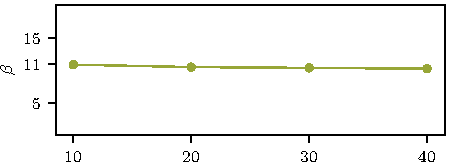
\includegraphics[width=\linewidth]{figures/fast-path-beta.pdf}
%     \captionof{figure}{An example of $\beta$ solutions for different $k$, with $n = 2000, \alpha = 0.8k$.}
%     \label{fig:fast-path-beta}
% \end{figure}
%O \noindent Overall, a very small number of iterations are sufficient for the safe early commitment predicate. This supports the choice of $\beta$ in our evaluation.

\noindent Globalement, un très petit nombre d'itérations est suffisant pour le prédicat d'engagement préalable sûr. Cela confirme le choix de $\beta$ dans notre évaluation.

%O \subsection{Initialization Heuristic}
\subsection{Heuristique d'initialisation}
\label{sec:sync-heuristic}
%O To improve liveness, we can use strong synchrony assumptions. The heuristic works as follows. Every node operates in two phases: in the first phase, it gossips and collects proposals for $\Oh{\log{n}}$ rounds, where each round lasts for the maximum message delay, which ensures the proposal from a correct node will propagate to almost all other correct nodes; in the second phase, each node stops collecting proposals, and gossips the existing proposals for an additional $\Oh{\log{n}}$ rounds so that every correct node ends up with approximately the same set of proposals. Finally, each node samples for the proposals it knows of locally, checking for those that have an $\alpha$ majority, ordered deterministically, such as by hash values. It then selects the first value by the order as its initial state when it starts the actual consensus protocol.
Pour améliorer la vitalité, nous pouvons utiliser des hypothèses de forte synchronie. L'heuristique fonctionne comme suit. Chaque nœud opère en deux phases\,: dans la première, elle diffuse et collecte des propositions pendant $\Oh{\log{n}}$ tours, où chaque tour dure le temps maximum d'un message, ce qui garantit que la proposition d'un nœud correct se propage vers presque tous les autres nœuds corrects\,; dans la se\-conde phase, chaque nœud arrête de collecter les propositions dont il a localement la connaissance, en recherchant ceux qui ont une majorité $\alpha$, ordonnée de manière déterministe, comme par la valeur de leur empreinte cryptographique. Il sélectionne ensuite la première valeur dans l'ordre pour en faire son état initial quand il commence vraiment le protocole de consensus.
%O In a cryptocurrency setting, the deterministic ordering function would incorporate fees paid out for every new proposal, which means that the adversary is financially limited in its ability to launch a fairness attack against the initialization.
Dans le cas d'une cryptomonnaie, la fonction de tri déterministe incorporerait les frais payés pour toute nouvelle proposition, ce qui signifie que l'adversaire serait financièrement limité pour lancer une attaque d'impartialité contre l'initialisation.

%O \subsection{Churn and View Discrepancy}\label{sec:full-analysis-churn}
\subsection{Roulement et incohérence de vues}\label{sec:full-analysis-churn}

%O Realistic systems need to accommodate the departure and arrival of nodes.
Les systèmes réalistes doivent s'accommoder du départ et de l'arrivée des nœuds.
%O Up to now, we simplified our analysis by assuming a precise knowledge of network membership, i.e. $\mathcal{L}(u) = \mathcal{N}$.
Jusqu'à présent, nous avons simplifié notre analyse en supposant une connaissance précise des membres du réseau, c'est-à-dire $\mathcal{L}(u) = \mathcal{N}$.
%O We now demonstrate that correct nodes can admit a well-characterized amount of churn, by showing how to pick parameters such that Avalanche nodes can differ in their view of the network and still safely make decisions.
Nous allons maintenant démontrer que les nœuds corrects peuvent admettre un roulement caractérisé d'entrants et de sortants en montrant comment choisir des paramètres tels que les nœuds Avalanche puissent différer dans leurs vues respectives du réseau tout en maintenant leur capacité à prendre des décisions en toute sécurité.

{\color{black} 

%O To characterize churn we use a generalized set intersection construction that allows us to make arguments about worst-case network view splits. Before formalizing it, we provide the intuition: suppose we split the network into two entirely independent, but fully connected, subsets. Clearly, the Byzantine adversary wins with probability one since it can send two conflicting transactions to the two independent networks respectively, and they would finalize the transactions immediately. This represents the worst case view split. 
Pour caractériser le roulement, nous utilisons une construction généralisée d'intersection d'ensembles qui nous permet d'établir des arguments concernant les éclatements de vues du réseau. Avant de le formaliser, nous partons de cette intuition\,: supposons que nous éclations le réseau en deux sous-ensembles entièrement indépendants mais parfaitement connectés. Il est clair que l'adversaire byzantin gagne avec une probabilité de un puisqu'il peut envoyer deux transactions conflictuelles à chaque réseau indépendant, et chacun fina\-liserait immédiatement les transactions. Cela représente le cas d'éclatement le plus défavorable.
\begin{figure}
\centering
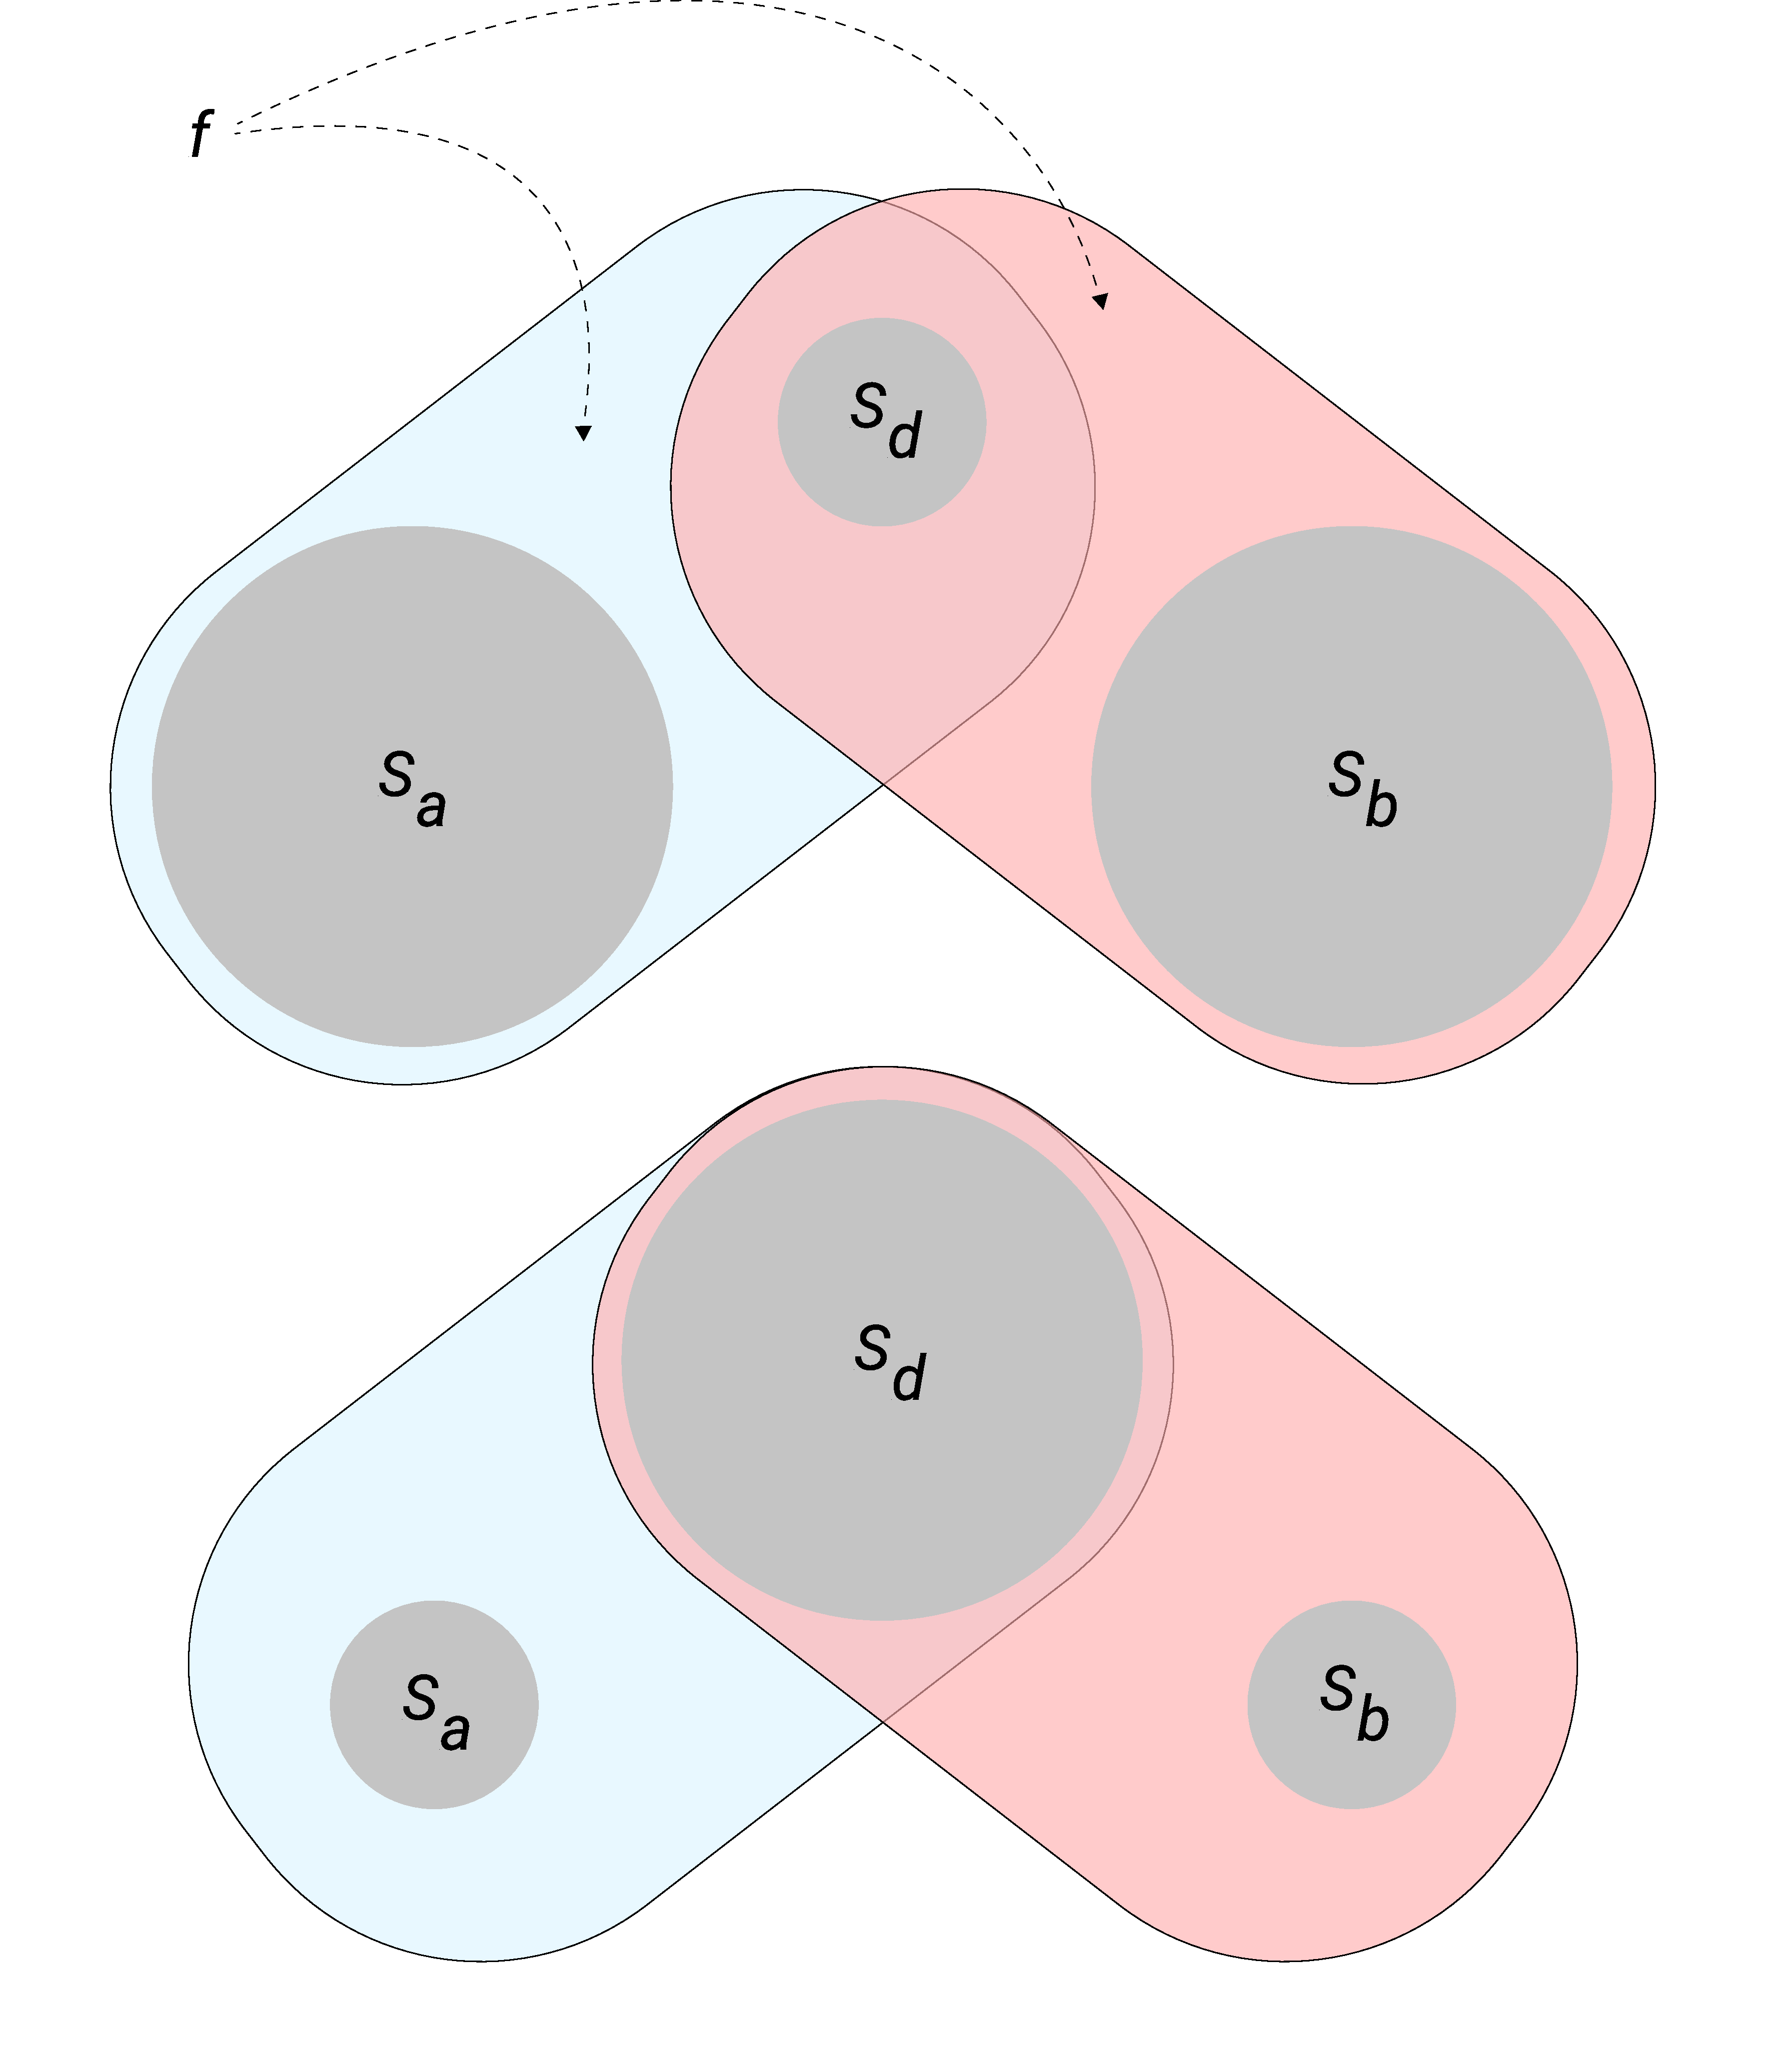
\includegraphics[width=0.8\linewidth]{figures/network_view.pdf}
%O \caption{Changes in network view based on $S_d$'s size. All prior proofs up to now represent the variant where $S_a = S_b = \emptyset$. With the new construction, the probability of safety violation is simply a direct application of the prior sets of proofs under the new subsets.}
\caption{Changements de la vue du réseau en se basant sur la taille de $S_d$. Toutes les preuves antérieures jusqu'à présent représentent la variante où $S_a = S_b = \emptyset$. Avec la nouvelle construction, la probabilité de violation de la sécurité de fonctionnement n'est qu'une application directe des ensembles antérieurs de preuves pour les nouveaux sous-ensembles.}
\label{fig:network_view}
\end{figure}
%O We can generalize this to arbitrary network splits, which can even be applied recursively in each subset. The proofs of safety then are a matter of characterizing the probability of red and blue committing into the two (possibly independent) subsets.
Nous pouvons généraliser ceci à d'autres éclatements du réseau, et même récursivement dans chaque sous-ensemble. Les preuves de sûreté de fonctionnement sont alors une question de caractérisation de la probabilité que les rouges et les bleus s'engagent dans les deux sous-ensembles (éventuellement indépendants).

%O Suppose we divide the set of correct nodes into three subsets, $S_a$, $S_d$, $S_b$. We overload $\mathcal{L}(S_{*})$ to represent the views of any node within the input set. The view of all nodes in $S_a$ is $\mathcal{L}(S_a) = S_a \cup S_d \cup \mathcal{B}$, the view of all nodes in $S_b$ is $\mathcal{L}(S_b) = S_b \cup S_d \cup \mathcal{B}$, and the view of $S_d$ is $\mathcal{N}$. We assume the worst case, which means that adversarial nodes are common to all subsets. When $S_d = \emptyset$, this represents a division of the network into two equal subsets where $|S_a| = |S_b| = n/2$~\footnote{$|S_a|$ and $|S_b|$ do not have to be equal, we assume so as a demonstration.}. If $S_d$ is all correct nodes, then $|S_a| = |S_b| = n$. This construction is visually demonstrated in Figure~\ref{fig:network_view}. 
Supposons que nous divisions l'ensemble de nœuds corrects en trois sous-ensembles, $S_a$, $S_d$, $S_b$. Nous surchargeons $\mathcal{L}(S_{*})$ pour représenter les vues de tout nœud dans l'ensemble d'entrées. La vue de tous les nœuds dans $S_a$ est $\mathcal{L}(S_a) = S_a \cup S_d \cup \mathcal{B}$, celle de tous les nœuds dans $S_b$ est $\mathcal{L}(S_b) = S_b \cup S_d \cup \mathcal{B}$, et la vue de $S_d$ est $\mathcal{N}$. Nous supposons le cas le plus défavorable, ce qui signifie que les nœuds de l'adversaire sont communs à tous les sous-ensembles. Quand $S_d = \emptyset$, cela représente une division du réseau en deux sous-ensembles égaux où $|S_a| = |S_b| = n/2$~\footnote{$|S_a|$ et $|S_b|$ ne sont pas nécessairement égaux, nous posons ceci pour la démonstration.}. Si $S_d$ est uniquement composé de nœuds corrects, alors $|S_a| = |S_b| = n$. Cette construction est démontrée visuellement en figure~\ref{fig:network_view}.

\begin{lemma}
%O Let $\tau \in \mathbb{Z}^{+}$. Let $|S_d| = n - \tau$, and thus $|S_{\{a, b\}}| = \tau/2$. There exists some maximal size of $\tau$ such that probability of any two nodes $u, v \in S_a,\ S_b,\ S_d$ finalizing equivocating transactions is less than $\epsilon$. 
Soit $\tau \in \mathbb{Z}^{+}$. Soit $|S_d| = n - \tau$, et donc $|S_{\{a, b\}}| = \tau/2$. Il existe un taille maximale de $\tau$ telle que la probabilité pour que deux nœuds quelconques $u, v \in S_a,\ S_b,\ S_d$ finalisant des transactions équivoques soit inférieuire à $\epsilon$. 
\end{lemma}
\begin{proof}
%O We assume that the adversary has full control of the network view splits, meaning that they choose in full how to create $S_a,\ S_b,\ S_d$. To prove safety, we simply reuse the same exact construction as in Subsection~\ref{subsection:appendix_snowflake}, but we replace the original set $\mathcal{N}$ with a new set of interest, namely $S_a \cup S_d \cup \mathcal{B}$ (i.e., we exclude $S_b$)~\footnote{Sets are symmetric in this example.}. To thus find the maximal $\tau$, we simply replace $u_i$ and $\lambda_i$ with 
Nous supposons que l'adversaire a le contrôle total des éclatements de la vue du réseau, ce qui signifie qu'il peut choisir sans contrainte de créer $S_a,\ S_b,\ S_d$. Pour prouver la sécurité de fonctionnement, il nous suffit de réutiliser exac\-tement la même construction qu'en section~\ref{subsection:appendix_snowflake}, mais nous remplaçons l'ensemble originel $\mathcal{N}$ avec le nouvel ensemble qui nous intéresse, nommément $S_a \cup S_d \cup \mathcal{B}$ (c'est-à-dire que nous excluons $S_b$)~\footnote{Les ensembles sont symétriques dans cet exemple.}. Donc, pour trouver le $\tau$ maximal, nous nous contentons de remplacer $u_i$ et $\lambda_i$ par
\begin{equation}
    \begin{cases}
        \bar \mu_i = i\ \mathcal{H}(S_a \cup S_d \cup \mathcal{B}, c-(\tau/2)-i, k, \alpha), & \text{for } i \rightarrow i - 1 \\
        \lambda_i = (c-i)\ \mathcal{H}(S_a \cup S_d \cup \mathcal{B}, i, k, \alpha), & \text{for } j \rightarrow i + 1 \\
    \end{cases}
\end{equation}
où
\begin{equation}
\begin{split}
P(\mathcal{H}&(S_a \cup S_d \cup \mathcal{B}, x, k) \geq \alpha)\\
&= \left.\sum_{j = \alpha}^{k} {x \choose j}{c-(\tau/2)-x \choose k-j}\middle/{c - (\tau/2) \choose k}\right.\\
\end{split}
\end{equation}
%O and apply the same construction as in Subsection~\ref{subsection:appendix_snowflake}. As $\tau$ increases, it is clear that $S_a$ (and conversely, $S_b$), become more independent and less reliant on the values proposed by members in $S_d$, thus incrementing the ability of the adversaries. 
et nous appliquons la même construction qu'en section~\ref{subsection:appendix_snowflake}. Alors que $\tau$ augmente, il est clair que $S_a$ (et, réciproquement, $S_b$) deviennent plus indépendants et moins dépendents des valeurs proposées par les membres de $S_d$, augmentant ainsi les capacités de l'adversaire.
\end{proof}


}


% Consider a network whose operation is divided into epochs of length $\tau$, and a view update from epoch $t$ to $t+1$ during which $\gamma$ nodes join the network and $\bar \gamma$ nodes depart.
% Under our static construction, the state space $\mathcal{S}_t$ of the network had a key parameter $\Delta^{t}$ at time $t$, induced by $c^{t}, f^{t}, n^{t}$ and the chosen security parameters.
% Churn can, at worst, impact the network by adding $\gamma$ nodes of color $\mathtt{B}$, and remove $\bar \gamma$ nodes of color $\mathtt{R}$.
% At time $t+1$, $n^{t+1} = n^{t} + \gamma - {\bar \gamma}$, while $f^{t+1}$ and $c^{t+1}$ will be modified by an amount $\leq \gamma - {\bar \gamma}$, and thus induce a new $\Delta^{t+1}$ for the chosen security parameters.
% This new $\Delta^{t+1}$ has to be chosen such that the probability of reversibility from state $c^{t+1}/2 + \Delta^{t+1} - \gamma$ is $\leq \varepsilon$, which ensures that the system will converge under the previous pessimal assumptions. The system designer can easily do this by picking an upper bound on $\gamma, \bar \gamma$.

% The final step in assuring the correctness of a view change is to account for a mix of nodes that straddle the $\tau$ boundary. We would like the network to avoid an unsafe state no matter which nodes are using the old and the new views.
% The easiest way to do this is to determine $\Delta^t$ and $\Delta^{t+1}$ for desired bounds on $\gamma, \bar \gamma$, and then to use the conservative value $\Delta^{t+1}$ during epoch $t$. In essence, this ensures that no commitments are made in configuration $\mathcal{S}_t$ unless they conservatively fulfill the safety criteria in state space $\mathcal{S}_{t+1}$. As a result, there is no possibility of a node deciding red at time $t$, the network going through an epoch change and finding itself to the left of the new irreversibility state $\Delta^{t+1}$.

% This approach trades off some of the feasibility space, to add the ability to accommodate $\gamma, \bar \gamma$ node churn per epoch.
% Overall, if $\tau$ is in excess of the time required for a decision (on the order of minutes to hours), and nodes are loosely synchronized,
% they can add or drop up to $\gamma, \bar \gamma$ nodes in each epoch using the conservative process described above.
% % Due to space reasons,
% We leave the precise method of entering and exiting the network by staking and unstaking to a subsequent paper, and instead
% rely on a membership oracle that acts as a sequencer and $\gamma$-rate-limiter, using technologies like Fireflies~\cite{JohansenRVJ15}.
% and Ethereum~\cite{wood2014ethereum}.
\end{appendices}
\end{document}
